% Формат А4, 14pt (ГОСТ Р 7.0.11-2011, 5.3.6)
\documentclass[a4paper,14pt]{extreport}

%%% Проверка используемого TeX-движка %%%
\usepackage{iftex}
\newif\ifxetexorluatex   % определяем новый условный оператор (http://tex.stackexchange.com/a/47579/79756)
\ifXeTeX
    \xetexorluatextrue
\else
    \ifLuaTeX
        \xetexorluatextrue
    \else
        \xetexorluatexfalse
    \fi
\fi

%%% Поля и разметка страницы %%%
\usepackage{pdflscape}                              % Для включения альбомных страниц
\usepackage{geometry}                               % Для последующего задания полей

%%% Математические пакеты %%%
\usepackage{amsthm,amsfonts,amsmath,amssymb,amscd}  % Математические дополнения от AMS
\usepackage{mathtools}                              % Добавляет окружение multlined

%%%% Установки для размера шрифта 14 pt %%%%
%% Формирование переменных и констант для сравнения (один раз для всех подключаемых файлов)%%
%% должно располагаться до вызова пакета fontspec или polyglossia, потому что они сбивают его работу
\newlength{\curtextsize}
\newlength{\bigtextsize}
\setlength{\bigtextsize}{13.9pt}

\makeatletter
%\show\f@size                                       % неплохо для отслеживания, но вызывает стопорение процесса, если документ компилируется без команды  -interaction=nonstopmode 
\setlength{\curtextsize}{\f@size pt}
\makeatother

%%% Кодировки и шрифты %%%
\ifxetexorluatex
    \usepackage{polyglossia}                        % Поддержка многоязычности (fontspec подгружается автоматически)
\else
    \RequirePDFTeX                                  % tests for PDFTEX use and throws an error if a different engine is being used
   %%% Решение проблемы копирования текста в буфер кракозябрами
%    \input glyphtounicode.tex
%    \input glyphtounicode-cmr.tex %from pdfx package
%    \pdfgentounicode=1
    \usepackage{cmap}                               % Улучшенный поиск русских слов в полученном pdf-файле
    \defaulthyphenchar=127                          % Если стоит до fontenc, то переносы не впишутся в выделяемый текст при копировании его в буфер обмена
    \usepackage[T2A]{fontenc}                       % Поддержка русских букв
    \usepackage[utf8]{inputenc}                     % Кодировка utf8
    \usepackage[english, russian]{babel}            % Языки: русский, английский
    \IfFileExists{pscyr.sty}{\usepackage{pscyr}}{}  % Красивые русские шрифты
\fi

%%% Оформление абзацев %%%
\usepackage{indentfirst}                            % Красная строка

%%% Цвета %%%
\usepackage[dvipsnames,usenames]{color}
\usepackage{colortbl}
%\usepackage[dvipsnames, table, hyperref, cmyk]{xcolor} % Вероятно, более новый вариант, вместо предыдущих двух строк. Конвертация всех цветов в cmyk заложена как удовлетворение возможного требования типографий. Возможно конвертирование и в rgb.

%%% Таблицы %%%
\usepackage{longtable}                              % Длинные таблицы
\usepackage{multirow,makecell,array}                % Улучшенное форматирование таблиц
\usepackage{booktabs}                               % Возможность оформления таблиц в классическом книжном стиле (при правильном использовании не противоречит ГОСТ)

%%% Общее форматирование
\usepackage{soulutf8}                               % Поддержка переносоустойчивых подчёркиваний и зачёркиваний
\usepackage{icomma}                                 % Запятая в десятичных дробях


%%% Гиперссылки %%%
\usepackage{hyperref}

%%% Изображения %%%
\usepackage{graphicx}                               % Подключаем пакет работы с графикой

%%% Списки %%%
\usepackage{enumitem}

%%% Подписи %%%
\usepackage{caption}                                % Для управления подписями (рисунков и таблиц) % Может управлять номерами рисунков и таблиц с caption %Иногда может управлять заголовками в списках рисунков и таблиц
\usepackage{subcaption}                             % Работа с подрисунками и подобным

%%% Интервалы %%%
\usepackage[onehalfspacing]{setspace}               % Опция запуска пакета правит не только интервалы в обычном тексте, но и формульные

%%% Счётчики %%%
\usepackage[figure,table]{totalcount}               % Счётчик рисунков и таблиц
\usepackage{totcount}                               % Пакет создания счётчиков на основе последнего номера подсчитываемого элемента (может требовать дважды компилировать документ)
\usepackage{totpages}                               % Счётчик страниц, совместимый с hyperref (ссылается на номер последней страницы). Желательно ставить последним пакетом в преамбуле
\usepackage{cleveref}
\creflabelformat{equation}{#2#1#3} 
  % Пакеты общие для диссертации и автореферата
%%% Прикладные пакеты %%% 
%\usepackage{calc}               % Пакет для расчётов параметров, например длины         % Пакеты для диссертации
%%% Микротипографика %%%
\ifnumequal{\value{draft}}{0}{% Только если у нас режим чистовика
    \usepackage[final]{microtype}[2016/05/14] % улучшает представление букв и слов в строках, может помочь при наличии отдельно висящих слов
}{}
        % Пакеты для специфических пользовательских задач

%%%%%%%%%%%%%%%%%%%%%%%%%%%%%%%%%%%%%%%%%%%%%%%%%%%%%%
%%%% Файл упрощённых настроек шаблона диссертации %%%%
%%%%%%%%%%%%%%%%%%%%%%%%%%%%%%%%%%%%%%%%%%%%%%%%%%%%%%

%%% Инициализирование переменных, не трогать!  %%%
\newcounter{intvl}
\newcounter{otstup}
\newcounter{contnumeq}
\newcounter{contnumfig}
\newcounter{contnumtab}
\newcounter{pgnum}
\newcounter{chapstyle}
\newcounter{headingdelim}
\newcounter{headingalign}
\newcounter{headingsize}
\newcounter{tabcap}
\newcounter{tablaba}
\newcounter{tabtita}
%%%%%%%%%%%%%%%%%%%%%%%%%%%%%%%%%%%%%%%%%%%%%%%%%%

%%% Область упрощённого управления оформлением %%%

%% Интервал между заголовками и между заголовком и текстом
% Заголовки отделяют от текста сверху и снизу тремя интервалами (ГОСТ Р 7.0.11-2011, 5.3.5)
\setcounter{intvl}{3}               % Коэффициент кратности к размеру шрифта

%% Отступы у заголовков в тексте
\setcounter{otstup}{0}              % 0 --- без отступа; 1 --- абзацный отступ

%% Нумерация формул, таблиц и рисунков
\setcounter{contnumeq}{0}           % Нумерация формул: 0 --- пораздельно (во введении подряд, без номера раздела); 1 --- сквозная нумерация по всей диссертации
\setcounter{contnumfig}{0}          % Нумерация рисунков: 0 --- пораздельно (во введении подряд, без номера раздела); 1 --- сквозная нумерация по всей диссертации
\setcounter{contnumtab}{1}          % Нумерация таблиц: 0 --- пораздельно (во введении подряд, без номера раздела); 1 --- сквозная нумерация по всей диссертации

%% Оглавление
\setcounter{pgnum}{1}               % 0 --- номера страниц никак не обозначены; 1 --- Стр. над номерами страниц (дважды компилировать после изменения)
\settocdepth{subsection}            % до какого уровня подразделов выносить в оглавление
\setsecnumdepth{subsection}         % до какого уровня нумеровать подразделы


%% Текст и форматирование заголовков
\setcounter{chapstyle}{1}           % 0 --- разделы только под номером; 1 --- разделы с названием "Глава" перед номером
\setcounter{headingdelim}{1}        % 0 --- номер отделен пропуском в 1em или \quad; 1 --- номера разделов и приложений отделены точкой с пробелом, подразделы пропуском без точки; 2 --- номера разделов, подразделов и приложений отделены точкой с пробелом.

%% Выравнивание заголовков в тексте
\setcounter{headingalign}{0}        % 0 --- по центру; 1 --- по левому краю

%% Размеры заголовков в тексте
\setcounter{headingsize}{0}         % 0 --- по ГОСТ, все всегда 14 пт; 1 --- пропорционально изменяющийся размер в зависимости от базового шрифта

%% Подпись таблиц
\setcounter{tabcap}{0}              % 0 --- по ГОСТ, номер таблицы и название разделены тире, выровнены по левому краю, при необходимости на нескольких строках; 1 --- подпись таблицы не по ГОСТ, на двух и более строках, дальнейшие настройки: 
%Выравнивание первой строки, с подписью и номером
\setcounter{tablaba}{2}             % 0 --- по левому краю; 1 --- по центру; 2 --- по правому краю
%Выравнивание строк с самим названием таблицы
\setcounter{tabtita}{1}             % 0 --- по левому краю; 1 --- по центру; 2 --- по правому краю

%%% Цвета гиперссылок %%%
% Latex color definitions: http://latexcolor.com/
% \definecolor{linkcolor}{rgb}{0.9,0,0}
% \definecolor{citecolor}{rgb}{0,0.6,0}
% \definecolor{urlcolor}{rgb}{0,0,1}
\definecolor{linkcolor}{rgb}{0,0,0} %black
\definecolor{citecolor}{rgb}{0,0,0} %black
\definecolor{urlcolor}{rgb}{0,0,0} %black               % Упрощённые настройки шаблона 

\input{preamblenames}       % Переопределение именований, чтобы можно было и в преамбуле использовать
%%% Основные сведения %%%
\newcommand{\thesisAuthor}             % Диссертация, ФИО автора
{%
    \texorpdfstring{% \texorpdfstring takes two arguments and uses the first for (La)TeX and the second for pdf
        Ладутенко Константин Сергеевич % так будет отображаться на титульном листе или в тексте, где будет использоваться переменная
    }{%
        Ладутенко, Константин Сергеевич% эта запись для свойств pdf-файла. В таком виде, если pdf будет обработан программами для сбора библиографических сведений, будет правильно представлена фамилия.
    }%
}
\newcommand{\thesisUdk}                % Диссертация, УДК
{\todo{xxx.xxx}}

\newcommand{\thesisTitleBoth}          % Диссертация, название
% {Моделирование взаимодействия оптимизированной многослойной сферы с
% плоской электромагнитной волной}
{Рассеяние и поглощение электромагнитных волн многослойными
сферическими порытиями}

\newcommand{\thesisTitle}              % Диссертация, название
{\texorpdfstring{\MakeUppercase{\thesisTitleBoth}}{\thesisTitleBoth}}

\newcommand{\thesisSpecialtyNumberBoth}    % Диссертация, специальность, номер
{01.04.05}
\newcommand{\thesisSpecialtyNumber}    % Диссертация, специальность, номер
{\texorpdfstring{\todo{\thesisSpecialtyNumberBoth}}{\thesisSpecialtyNumberBoth}}

\newcommand{\thesisSpecialtyTitleBoth}     % Диссертация, специальность, название
{Оптика}
\newcommand{\thesisSpecialtyTitle}     % Диссертация, специальность, название
{\texorpdfstring{\todo{\thesisSpecialtyTitleBoth}}{\thesisSpecialtyTitleBoth}}


% \newcommand{\thesisSpecialtyNumberBothSecond}    % Диссертация, специальность, номер
% {05.13.18}
% \newcommand{\thesisSpecialtyNumberSecond}    % Диссертация, специальность, номер
% {\texorpdfstring{\todo{\thesisSpecialtyNumberBothSecond}}{\thesisSpecialtyNumberBothSecond}}

% \newcommand{\thesisSpecialtyTitleBothSecond}     % Диссертация, специальность, название
% { Математическое моделирование, численные методы и комплексы программ}
% \newcommand{\thesisSpecialtyTitleSecond}     % Диссертация, специальность, название
% {\texorpdfstring{\todo{\thesisSpecialtyTitleBothSecond}}{\thesisSpecialtyTitleBothSecond}}



\newcommand{\thesisDegree}             % Диссертация, научная степень
{кандидата физико-математических наук}
\newcommand{\thesisCity}               % Диссертация, город защиты
{Санкт-Петербург}
\newcommand{\thesisYear}               % Диссертация, год защиты
{\todo{20XX}}
\newcommand{\thesisOrganization}       % Диссертация, организация
{Федеральное государственное автономное образовательное учреждение высшего образования <<Санкт-Петербургский национальный исследовательский университет информационных технологий, механики и оптики>>}

\newcommand{\thesisInOrganization}       % Диссертация, организация в предложном падеже: Работа выполнена в ...
{федеральном государственном автономном образовательном учреждении высшего образования <<Санкт-Петербургский национальный исследовательский университет информационных технологий, механики и оптики>>}

\newcommand{\supervisorFio}            % Научный руководитель, ФИО
{Белов Павел Александрович}
\newcommand{\supervisorRegalia}        % Научный руководитель, регалии
{\todo{доктор физико-математических наук}}

\newcommand{\opponentOneFio}           % Оппонент 1, ФИО
{\todo{Фамилия Имя Отчество}}
\newcommand{\opponentOneRegalia}       % Оппонент 1, регалии
{\todo{доктор физико-математических наук, профессор}}
\newcommand{\opponentOneJobPlace}      % Оппонент 1, место работы
{\todo{Не очень длинное название для места работы}}
\newcommand{\opponentOneJobPost}       % Оппонент 1, должность
{\todo{старший научный сотрудник}}

\newcommand{\opponentTwoFio}           % Оппонент 2, ФИО
{\todo{Фамилия Имя Отчество}}
\newcommand{\opponentTwoRegalia}       % Оппонент 2, регалии
{\todo{кандидат физико-математических наук}}
\newcommand{\opponentTwoJobPlace}      % Оппонент 2, место работы
{\todo{Основное место работы c длинным длинным длинным длинным названием}}
\newcommand{\opponentTwoJobPost}       % Оппонент 2, должность
{\todo{старший научный сотрудник}}

\newcommand{\leadingOrganizationTitle} % Ведущая организация, дополнительные строки
{\todo{Федеральное государственное бюджетное образовательное учреждение высшего профессионального образования с~длинным длинным длинным длинным названием}}

\newcommand{\defenseDate}              % Защита, дата
{\todo{DD mmmmmmmm YYYY~г.~в~XX часов}}
\newcommand{\defenseCouncilNumber}     % Защита, номер диссертационного совета
{\todo{NN}}
\newcommand{\defenseCouncilTitle}      % Защита, учреждение диссертационного совета
{\todo{Название учреждения}}
\newcommand{\defenseCouncilAddress}    % Защита, адрес учреждение диссертационного совета
{\todo{Адрес}}

\newcommand{\defenseSecretaryFio}      % Секретарь диссертационного совета, ФИО
{\todo{Фамилия Имя Отчество}}
\newcommand{\defenseSecretaryRegalia}  % Секретарь диссертационного совета, регалии
{\todo{д-р~физ.-мат. наук}}            % Для сокращений есть ГОСТы, например: ГОСТ Р 7.0.12-2011 + http://base.garant.ru/179724/#block_30000

\newcommand{\synopsisLibrary}          % Автореферат, название библиотеки
{\todo{Название библиотеки}}
\newcommand{\synopsisDate}             % Автореферат, дата рассылки
{\todo{DD mmmmmmmm YYYY года}}

\newcommand{\keywords}%                 % Ключевые слова для метаданных PDF диссертации и автореферата
{}
      % Основные сведения
%%% Кодировки и шрифты %%%
\ifxetexorluatex
    \setmainlanguage[babelshorthands=true]{russian}  % Язык по-умолчанию русский с поддержкой приятных команд пакета babel
    \setotherlanguage{english}                       % Дополнительный язык = английский (в американской вариации по-умолчанию)
    \setmonofont{Courier New}
    \newfontfamily\cyrillicfonttt{Courier New}
    \ifXeTeX
        \defaultfontfeatures{Ligatures=TeX,Mapping=tex-text}
    \else
        \defaultfontfeatures{Ligatures=TeX}
    \fi
    \setmainfont{Times New Roman}
    \newfontfamily\cyrillicfont{Times New Roman}
    \setsansfont{Arial}
    \newfontfamily\cyrillicfontsf{Arial}
\else
    \IfFileExists{pscyr.sty}{\renewcommand{\rmdefault}{ftm}}{}
\fi

%%% Выравнивание и переносы %%%
%% http://tex.stackexchange.com/questions/241343/what-is-the-meaning-of-fussy-sloppy-emergencystretch-tolerance-hbadness
%% http://www.latex-community.org/forum/viewtopic.php?p=70342#p70342
\tolerance 1414
\hbadness 1414
\emergencystretch 1em %поиграться стоит
\hfuzz 0.3pt
\vfuzz \hfuzz
%\raggedbottom
%\sloppy                             % Избавляемся от переполнений
\clubpenalty=10000                  % Запрещаем разрыв страницы после первой строки абзаца
\widowpenalty=10000                 % Запрещаем разрыв страницы после
                                % последней строки абзаца

% %%% Выравнивание и переносы %%%
% \sloppy                             % Избавляемся от переполнений
% \clubpenalty=10000                  % Запрещаем разрыв страницы после первой строки абзаца
% \widowpenalty=10000                 % Запрещаем разрыв страницы после последней строки абзаца
% %\righthyphenmin=2 %Разрешаем перенос двух букв
% \tolerance=500 \hyphenpenalty=100 \doublehyphendemerits=50000
% \finalhyphendemerits=10000 \brokenpenalty=10000 

%%% Подписи %%%
\captionsetup{%
singlelinecheck=off,                % Многострочные подписи, например у таблиц
skip=2pt,                           % Вертикальная отбивка между подписью и содержимым рисунка или таблицы определяется ключом
justification=centering,            % Центрирование подписей, заданных командой \caption
}

%%% Рисунки %%%
\DeclareCaptionLabelSeparator*{emdash}{~--- }             % (ГОСТ 2.105, 4.3.1)
\captionsetup[figure]{labelsep=emdash,position=bottom}

%%% Таблицы %%%
\ifnumequal{\value{tabcap}}{0}{%
    \newcommand{\tabcapalign}{\raggedright}  % по левому краю страницы или аналога parbox

    \DeclareCaptionFormat{tablecaption}{\tabcapalign #1#2#3}
    \captionsetup[table]{labelsep=emdash}                       % тире как разделитель идентификатора с номером от наименования
}{%
    \ifnumequal{\value{tablaba}}{0}{%
        \newcommand{\tabcapalign}{\raggedright}  % по левому краю страницы или аналога parbox
    }{}

    \ifnumequal{\value{tablaba}}{1}{%
        \newcommand{\tabcapalign}{\centering}    % по центру страницы или аналога parbox
    }{}

    \ifnumequal{\value{tablaba}}{2}{%
        \newcommand{\tabcapalign}{\raggedleft}   % по правому краю страницы или аналога parbox
    }{}

    \ifnumequal{\value{tabtita}}{0}{%
        \newcommand{\tabtitalign}{\raggedright}  % по левому краю страницы или аналога parbox
    }{}

    \ifnumequal{\value{tabtita}}{1}{%
        \newcommand{\tabtitalign}{\centering}    % по центру страницы или аналога parbox
    }{}

    \ifnumequal{\value{tabtita}}{2}{%
        \newcommand{\tabtitalign}{\raggedleft}   % по правому краю страницы или аналога parbox
    }{}

    \DeclareCaptionFormat{tablecaption}{\tabcapalign #1#2\par%  % Идентификатор таблицы на отдельной строке
        \tabtitalign{#3}}                                       % Наименование таблицы строкой ниже
    \captionsetup[table]{labelsep=space}                        % пробельный разделитель идентификатора с номером от наименования
}
\DeclareCaptionFormat{tablenocaption}{\tabcapalign #1\strut}    % Наименование таблицы отсутствует

\captionsetup[table]{format=tablecaption,singlelinecheck=off,position=top,skip=0pt}  % многострочные наименования и прочее
\DeclareCaptionLabelFormat{continued}{Продолжение таблицы~#2}

%%% Подписи подрисунков %%%
\renewcommand{\thesubfigure}{\asbuk{subfigure}}           % Буквенные номера подрисунков
\captionsetup[subfigure]{font={normalsize},               % Шрифт подписи названий подрисунков (не отличается от основного)
    labelformat=brace,                                    % Формат обозначения подрисунка
    justification=centering,                              % Выключка подписей (форматирование), один из вариантов            
}
%\DeclareCaptionFont{font12pt}{\fontsize{12pt}{13pt}\selectfont} % объявляем шрифт 12pt для использования в подписях, тут же надо интерлиньяж объявлять, если не наследуется
%\captionsetup[subfigure]{font={font12pt}}                 % Шрифт подписи названий подрисунков (всегда 12pt)

%%% Настройки гиперссылок %%%
\ifLuaTeX
    \hypersetup{
        unicode,                % Unicode encoded PDF strings
    }
\fi

\hypersetup{
    linktocpage=true,           % ссылки с номера страницы в оглавлении, списке таблиц и списке рисунков
%    linktoc=all,                % both the section and page part are links
%    pdfpagelabels=false,        % set PDF page labels (true|false)
    plainpages=false,           % Forces page anchors to be named by the Arabic form  of the page number, rather than the formatted form
    colorlinks,                 % ссылки отображаются раскрашенным текстом, а не раскрашенным прямоугольником, вокруг текста
    linkcolor={linkcolor},      % цвет ссылок типа ref, eqref и подобных
    citecolor={citecolor},      % цвет ссылок-цитат
    urlcolor={urlcolor},        % цвет гиперссылок
%    hidelinks,                  % Hide links (removing color and border)
    pdftitle={\thesisTitle},    % Заголовок
    pdfauthor={\thesisAuthor},  % Автор
    pdfsubject={\thesisSpecialtyNumber\ \thesisSpecialtyTitle},      % Тема
%    pdfcreator={Создатель},     % Создатель, Приложение
%    pdfproducer={Производитель},% Производитель, Производитель PDF
    pdfkeywords={\keywords},    % Ключевые слова
    pdflang={ru},
}
\ifnumequal{\value{draft}}{1}{% Черновик
    \hypersetup{
        draft,
    }
}{}

%%% Шаблон %%%
\DeclareRobustCommand{\todo}{\textcolor{red}}       % решаем проблему превращения названия цвета в результате \MakeUppercase, http://tex.stackexchange.com/a/187930/79756 , \DeclareRobustCommand protects \todo from expanding inside \MakeUppercase
\AtBeginDocument{%
    \setlength{\parindent}{2.5em}                   % Абзацный отступ. Должен быть одинаковым по всему тексту и равен пяти знакам (ГОСТ Р 7.0.11-2011, 5.3.7).
}

%%% Списки %%%
% Используем короткое тире (endash) для ненумерованных списков (ГОСТ 2.105-95, пункт 4.1.7, требует дефиса, но так лучше смотрится)
\renewcommand{\labelitemi}{\normalfont\bfseries{--}}

% Перечисление строчными буквами латинского алфавита (ГОСТ 2.105-95, 4.1.7)
%\renewcommand{\theenumi}{\alph{enumi}}
%\renewcommand{\labelenumi}{\theenumi)} 

% Перечисление строчными буквами русского алфавита (ГОСТ 2.105-95, 4.1.7)
\makeatletter
\AddEnumerateCounter{\asbuk}{\russian@alph}{щ}      % Управляем списками/перечислениями через пакет enumitem, а он 'не знает' про asbuk, потому 'учим' его
\makeatother
%\renewcommand{\theenumi}{\asbuk{enumi}} %первый уровень нумерации
%\renewcommand{\labelenumi}{\theenumi)} %первый уровень нумерации 
\renewcommand{\theenumii}{\asbuk{enumii}} %второй уровень нумерации
\renewcommand{\labelenumii}{\theenumii)} %второй уровень нумерации 
\renewcommand{\theenumiii}{\arabic{enumiii}} %третий уровень нумерации
\renewcommand{\labelenumiii}{\theenumiii)} %третий уровень нумерации 

\setlist{nosep,%                                    % Единый стиль для всех списков (пакет enumitem), без дополнительных интервалов.
    labelindent=\parindent,leftmargin=*%            % Каждый пункт, подпункт и перечисление записывают с абзацного отступа (ГОСТ 2.105-95, 4.1.8)
}
    % Стили общие для диссертации и автореферата
%%% Изображения %%%
\graphicspath{{images/}{Dissertation/images/}}         % Пути к изображениям

\LoadInterface {titlesec}                   % Подгружаем интерфейсы для дополнительных опций управления некоторыми пакетами

%%% Блок управления параметрами для выравнивания заголовков в тексте %%%
\newlength{\otstuplen}
\setlength{\otstuplen}{\theotstup\parindent}
\ifthenelse{\equal{\theheadingalign}{0}}{% выравнивание заголовков в тексте
    \newcommand{\hdngalign}{\filcenter}                % по центру
    \newcommand{\hdngaligni}{\hfill\hspace{\otstuplen}}% по центру
}{%
    \newcommand{\hdngalign}{\filright}                 % по левому краю
    \newcommand{\hdngaligni}{\hspace{\otstuplen}}      % по левому краю
} % В обоих случаях вроде бы без переноса, как и надо (ГОСТ Р 7.0.11-2011, 5.3.5)

%%% Оглавление %%%
\renewcommand{\cftchapdotsep}{\cftdotsep}                % отбивка точками до номера страницы начала главы/раздела
\renewcommand{\cfttoctitlefont}{\hdngaligni\fontsize{14pt}{16pt}\selectfont\bfseries}% вместе со следующей строкой
\renewcommand{\cftaftertoctitle}{\hfill}                 % устанавливает заголовок по центру
\setlength{\cftbeforetoctitleskip}{-1.4\curtextsize}     % Поскольку этот заголовок всегда является первым на странице, то перед ним отделять пустым тройным интервалом не следует. Независимо от основного шрифта, в этом случае зануление (почти) происходит при -1.4\curtextsize.
\setlength{\cftaftertoctitleskip}{\theintvl\curtextsize} % Если считаем Оглавление заголовком, то выставляем после него тройной интервал через наше определённое значение

%% Переносить слова в заголовке не допускается (ГОСТ Р 7.0.11-2011, 5.3.5). Заголовки в оглавлении должны точно повторять заголовки в тексте (ГОСТ Р 7.0.11-2011, 5.2.3). Прямого указания на запрет переносов в оглавлении нет, но по той же логике невнесения искажений в смысл, лучше в оглавлении не переносить:
\cftsetrmarg{2.55em plus1fil}                       %To have the (sectional) titles in the ToC, etc., typeset ragged right with no hyphenation
\renewcommand{\cftchappagefont}{\normalfont}        % нежирные номера страниц у глав в оглавлении
\renewcommand{\cftchapleader}{\cftdotfill{\cftchapdotsep}}% нежирные точки до номеров страниц у глав в оглавлении
%\renewcommand{\cftchapfont}{}                       % нежирные названия глав в оглавлении

\ifthenelse{\theheadingdelim > 0}{%
    \renewcommand\cftchapaftersnum{.\ }   % добавляет точку с пробелом после номера раздела в оглавлении
}{%
\renewcommand\cftchapaftersnum{\quad}     % добавляет \quad после номера раздела в оглавлении
}
\ifthenelse{\theheadingdelim > 1}{%
    \renewcommand\cftsecaftersnum{.\ }    % добавляет точку с пробелом после номера подраздела в оглавлении
    \renewcommand\cftsubsecaftersnum{.\ } % добавляет точку с пробелом после номера подподраздела в оглавлении
}{%
\renewcommand\cftsecaftersnum{\quad}      % добавляет \quad после номера подраздела в оглавлении
\renewcommand\cftsubsecaftersnum{\quad}   % добавляет \quad после номера подподраздела в оглавлении
}

\ifthenelse{\equal{\thepgnum}{1}}{%
    \addtocontents{toc}{~\hfill{Стр.}\par}% добавить Стр. над номерами страниц
}

%%% Оформление названий глав %%%
%% настройки заголовка списка рисунков
\renewcommand{\cftloftitlefont}{\hdngaligni\fontsize{14pt}{16pt}\selectfont\bfseries}% вместе со следующей строкой
\renewcommand{\cftafterloftitle}{\hfill}                                             % устанавливает заголовок по центру
\setlength{\cftbeforeloftitleskip}{-1.5\curtextsize}     % Поскольку этот заголовок всегда является первым на странице, то перед ним отделять пустым тройным интервалом не следует. Независимо от основного шрифта, в этом случае зануление (почти) происходит при -1.5\curtextsize.
\setlength{\cftafterloftitleskip}{\theintvl\curtextsize} % выставляем после него тройной интервал через наше определённое значение

%% настройки заголовка списка таблиц
\renewcommand{\cftlottitlefont}{\hdngaligni\fontsize{14pt}{16pt}\selectfont\bfseries}% вместе со следующей строкой
\renewcommand{\cftafterlottitle}{\hfill}                                             % устанавливает заголовок по центру
\setlength{\cftbeforelottitleskip}{-1.5\curtextsize}     % Поскольку этот заголовок всегда является первым на странице, то перед ним отделять пустым тройным интервалом не следует. Независимо от основного шрифта, в этом случае зануление (почти) происходит при -1.5\curtextsize.
\setlength{\cftafterlottitleskip}{\theintvl\curtextsize} % выставляем после него тройной интервал через наше определённое значение

\ifnum\curtextsize>\bigtextsize     % Проверяем условие использования базового шрифта 14 pt
\setlength{\headheight}{17pt}       % Исправляем высоту заголовка
\else
\setlength{\headheight}{15pt}       % Исправляем высоту заголовка
\fi

%%% Колонтитулы %%%
% Порядковый номер страницы печатают на середине верхнего поля страницы (ГОСТ Р 7.0.11-2011, 5.3.8)
\makeatletter
\let\ps@plain\ps@fancy              % Подчиняем первые страницы каждой главы общим правилам
\makeatother
\pagestyle{fancy}                   % Меняем стиль оформления страниц
\fancyhf{}                          % Очищаем текущие значения
\fancyhead[C]{\thepage}             % Печатаем номер страницы на середине верхнего поля
\renewcommand{\headrulewidth}{0pt}  % Убираем разделительную линию

%%% Оформление заголовков глав, разделов, подразделов %%%
%% Работа должна быть выполнена ... размером шрифта 12-14 пунктов (ГОСТ Р 7.0.11-2011, 5.3.8). То есть не должно быть надписей шрифтом более 14. Так и поставим.
%% Эти установки будут давать одинаковый результат независимо от выбора базовым шрифтом 12 пт или 14 пт
\titleformat{\chapter}[block]                                % default display;  hang = with a hanging label. (Like the standard \section.); block = typesets the whole title in a block (a paragraph) without additional formatting. Useful in centered titles
        {\hdngalign\fontsize{14pt}{16pt}\selectfont\bfseries}% 
        %\fontsize{<size>}{<skip>} % второе число ставим 1.2*первое, чтобы адекватно отрабатывали команды по расчету полуторного интервала (домножая разные комбинации коэффициентов на этот)
        {\thechapter\cftchapaftersnum}                       % Заголовки в оглавлении должны точно повторять заголовки в тексте (ГОСТ Р 7.0.11-2011, 5.2.3).
        {0em}% отступ от номера до текста
        {}%

\titleformat{\section}[block]                                % default hang;  hang = with a hanging label. (Like the standard \section.); block = typesets the whole title in a block (a paragraph) without additional formatting. Useful in centered titles
        {\hdngalign\fontsize{14pt}{16pt}\selectfont\bfseries}% 
        %\fontsize{<size>}{<skip>} % второе число ставим 1.2*первое, чтобы адекватно отрабатывали команды по расчету полуторного интервала (домножая разные комбинации коэффициентов на этот)
        {\thesection\cftsecaftersnum}                        % Заголовки в оглавлении должны точно повторять заголовки в тексте (ГОСТ Р 7.0.11-2011, 5.2.3).
        {0em}% отступ от номера до текста
        {}%

\titleformat{\subsection}[block]                             % default hang;  hang = with a hanging label. (Like the standard \section.); block = typesets the whole title in a block (a paragraph) without additional formatting. Useful in centered titles
        {\hdngalign\fontsize{14pt}{16pt}\selectfont\bfseries}% 
        %\fontsize{<size>}{<skip>} % второе число ставим 1.2*первое, чтобы адекватно отрабатывали команды по расчету полуторного интервала (домножая разные комбинации коэффициентов на этот)
        {\thesubsection\cftsubsecaftersnum}                  % Заголовки в оглавлении должны точно повторять заголовки в тексте (ГОСТ Р 7.0.11-2011, 5.2.3).
        {0em}% отступ от номера до текста
        {}%

\ifthenelse{\equal{\thechapstyle}{1}}{%
    \sectionformat{\chapter}{% Параметры заголовков разделов в тексте
        label=\chaptername\ \thechapter\cftchapaftersnum,
        labelsep=0em,
    }
    %% Следующие две строки: будет вписано слово Глава перед каждым номером раздела в оглавлении   
    \renewcommand{\cftchappresnum}{\chaptername\ }
    \setlength{\cftchapnumwidth}{\widthof{\cftchapfont\cftchappresnum\thechapter\cftchapaftersnum}}
}%

%% Интервалы между заголовками
% На эти величины titlespacing множит через *
\beforetitleunit=\curtextsize% привязались к нашему размеру шрифта
\aftertitleunit=\curtextsize% привязались к нашему размеру шрифта

% Счётчик intvl и длина \otstup определены в файле setup
\titlespacing{\chapter}{\theotstup\parindent}{-1.7em}{*\theintvl}       % Заголовки отделяют от текста сверху и снизу тремя интервалами (ГОСТ Р 7.0.11-2011, 5.3.5). Поскольку название главы всегда является первым на странице, то перед ним отделять пустым тройным интервалом не следует. Независимо от основного шрифта, в этом случае зануление происходит при -1.7em.
\titlespacing{\section}{\theotstup\parindent}{*\theintvl}{*\theintvl}
\titlespacing{\subsection}{\theotstup\parindent}{*\theintvl}{*\theintvl}
\titlespacing{\subsubsection}{\theotstup\parindent}{*\theintvl}{*\theintvl}

%%% Блок дополнительного управления размерами заголовков
\ifthenelse{\equal{\theheadingsize}{1}}{% Пропорциональные заголовки и базовый шрифт 14 пт
    \renewcommand{\cfttoctitlefont}{\hdngaligni\Large\bfseries} % Исправляем размер заголовка оглавления
    \setlength{\cftbeforetoctitleskip}{-1.2\curtextsize}        % Исправляем вертикальный отступ перед заголовком оглавления
    \renewcommand{\cftloftitlefont}{\hdngaligni\Large\bfseries} % Исправляем размер заголовка списка рисунков
    \setlength{\cftbeforeloftitleskip}{-1.4\curtextsize}        % Исправляем вертикальный отступ перед заголовком списка рисунков
    \renewcommand{\cftlottitlefont}{\hdngaligni\Large\bfseries} % Исправляем размер заголовка списка таблиц 
    \setlength{\cftbeforelottitleskip}{-1.4\curtextsize}        % Исправляем вертикальный отступ перед заголовком списка таблиц
    \sectionformat{\chapter}{% Параметры заголовков разделов в тексте
        format=\hdngalign\Large\bfseries, % Исправляем размер заголовка
        top-=0.4em,                       % Исправляем вертикальный отступ перед заголовком
    }
    \sectionformat{\section}{% Параметры заголовков подразделов в тексте
        format=\hdngalign\large\bfseries, % Исправляем размер заголовка
    }
}

\ifthenelse{\equal{\theheadingsize}{1}\AND \curtextsize < \bigtextsize}{% Пропорциональные заголовки и базовый шрифт 14 пт
    \sectionformat{\chapter}{% Параметры заголовков разделов в тексте
        top-=0.2em, % Исправляем вертикальный отступ перед заголовком
    }
}

%%% Счётчики %%%

%% Упрощённые настройки шаблона диссертации: нумерация формул, таблиц, рисунков
\ifthenelse{\equal{\thecontnumeq}{1}}{%
    \counterwithout{equation}{chapter} % Убираем связанность номера формулы с номером главы/раздела
}
\ifthenelse{\equal{\thecontnumfig}{1}}{%
    \counterwithout{figure}{chapter}   % Убираем связанность номера рисунка с номером главы/раздела
}
\ifthenelse{\equal{\thecontnumtab}{1}}{%
    \counterwithout{table}{chapter}    % Убираем связанность номера таблицы с номером главы/раздела
}


%%http://www.linux.org.ru/forum/general/6993203#comment-6994589 (используется totcount)
\makeatletter
\def\formbytotal#1#2#3#4#5{%
    \newcount\@c
    \@c\totvalue{#1}\relax
    \newcount\@last
    \newcount\@pnul
    \@last\@c\relax
    \divide\@last 10
    \@pnul\@last\relax
    \divide\@pnul 10
    \multiply\@pnul-10
    \advance\@pnul\@last
    \multiply\@last-10
    \advance\@last\@c
    \total{#1}~#2%
    \ifnum\@pnul=1#5\else%
    \ifcase\@last#5\or#3\or#4\or#4\or#4\else#5\fi
    \fi
}
\makeatother

\AtBeginDocument{
%% регистрируем счётчики в системе totcounter
    \regtotcounter{totalcount@figure}
    \regtotcounter{totalcount@table}       % Если иным способом поставить в преамбуле то ошибка в числе таблиц
    \regtotcounter{TotPages}               % Если иным способом поставить в преамбуле то ошибка в числе страниц
}           % Стили для диссертации
% для вертикального центрирования ячеек в tabulary
\def\zz{\ifx\[$\else\aftergroup\zzz\fi}
\def\zzz{\setbox0\lastbox
\dimen0\dimexpr\extrarowheight + \ht0-\dp0\relax
\setbox0\hbox{\raise-.5\dimen0\box0}%
\ht0=\dimexpr\ht0+\extrarowheight\relax
\dp0=\dimexpr\dp0+\extrarowheight\relax 
\box0
}



\lstdefinelanguage{Renhanced}%
{keywords={abbreviate,abline,abs,acos,acosh,action,add1,add,%
        aggregate,alias,Alias,alist,all,anova,any,aov,aperm,append,apply,%
        approx,approxfun,apropos,Arg,args,array,arrows,as,asin,asinh,%
        atan,atan2,atanh,attach,attr,attributes,autoload,autoloader,ave,%
        axis,backsolve,barplot,basename,besselI,besselJ,besselK,besselY,%
        beta,binomial,body,box,boxplot,break,browser,bug,builtins,bxp,by,%
        c,C,call,Call,case,cat,category,cbind,ceiling,character,char,%
        charmatch,check,chol,chol2inv,choose,chull,class,close,cm,codes,%
        coef,coefficients,co,col,colnames,colors,colours,commandArgs,%
        comment,complete,complex,conflicts,Conj,contents,contour,%
        contrasts,contr,control,helmert,contrib,convolve,cooks,coords,%
        distance,coplot,cor,cos,cosh,count,fields,cov,covratio,wt,CRAN,%
        create,crossprod,cummax,cummin,cumprod,cumsum,curve,cut,cycle,D,%
        data,dataentry,date,dbeta,dbinom,dcauchy,dchisq,de,debug,%
        debugger,Defunct,default,delay,delete,deltat,demo,de,density,%
        deparse,dependencies,Deprecated,deriv,description,detach,%
        dev2bitmap,dev,cur,deviance,off,prev,,dexp,df,dfbetas,dffits,%
        dgamma,dgeom,dget,dhyper,diag,diff,digamma,dim,dimnames,dir,%
        dirname,dlnorm,dlogis,dnbinom,dnchisq,dnorm,do,dotplot,double,%
        download,dpois,dput,drop,drop1,dsignrank,dt,dummy,dump,dunif,%
        duplicated,dweibull,dwilcox,dyn,edit,eff,effects,eigen,else,%
        emacs,end,environment,env,erase,eval,equal,evalq,example,exists,%
        exit,exp,expand,expression,External,extract,extractAIC,factor,%
        fail,family,fft,file,filled,find,fitted,fivenum,fix,floor,for,%
        For,formals,format,formatC,formula,Fortran,forwardsolve,frame,%
        frequency,ftable,ftable2table,function,gamma,Gamma,gammaCody,%
        gaussian,gc,gcinfo,gctorture,get,getenv,geterrmessage,getOption,%
        getwd,gl,glm,globalenv,gnome,GNOME,graphics,gray,grep,grey,grid,%
        gsub,hasTsp,hat,heat,help,hist,home,hsv,httpclient,I,identify,if,%
        ifelse,Im,image,\%in\%,index,influence,measures,inherits,install,%
        installed,integer,interaction,interactive,Internal,intersect,%
        inverse,invisible,IQR,is,jitter,kappa,kronecker,labels,lapply,%
        layout,lbeta,lchoose,lcm,legend,length,levels,lgamma,library,%
        licence,license,lines,list,lm,load,local,locator,log,log10,log1p,%
        log2,logical,loglin,lower,lowess,ls,lsfit,lsf,ls,machine,Machine,%
        mad,mahalanobis,make,link,margin,match,Math,matlines,mat,matplot,%
        matpoints,matrix,max,mean,median,memory,menu,merge,methods,min,%
        missing,Mod,mode,model,response,mosaicplot,mtext,mvfft,na,nan,%
        names,omit,nargs,nchar,ncol,NCOL,new,next,NextMethod,nextn,%
        nlevels,nlm,noquote,NotYetImplemented,NotYetUsed,nrow,NROW,null,%
        numeric,\%o\%,objects,offset,old,on,Ops,optim,optimise,optimize,%
        options,or,order,ordered,outer,package,packages,page,pairlist,%
        pairs,palette,panel,par,parent,parse,paste,path,pbeta,pbinom,%
        pcauchy,pchisq,pentagamma,persp,pexp,pf,pgamma,pgeom,phyper,pico,%
        pictex,piechart,Platform,plnorm,plogis,plot,pmatch,pmax,pmin,%
        pnbinom,pnchisq,pnorm,points,poisson,poly,polygon,polyroot,pos,%
        postscript,power,ppoints,ppois,predict,preplot,pretty,Primitive,%
        print,prmatrix,proc,prod,profile,proj,prompt,prop,provide,%
        psignrank,ps,pt,ptukey,punif,pweibull,pwilcox,q,qbeta,qbinom,%
        qcauchy,qchisq,qexp,qf,qgamma,qgeom,qhyper,qlnorm,qlogis,qnbinom,%
        qnchisq,qnorm,qpois,qqline,qqnorm,qqplot,qr,Q,qty,qy,qsignrank,%
        qt,qtukey,quantile,quasi,quit,qunif,quote,qweibull,qwilcox,%
        rainbow,range,rank,rbeta,rbind,rbinom,rcauchy,rchisq,Re,read,csv,%
        csv2,fwf,readline,socket,real,Recall,rect,reformulate,regexpr,%
        relevel,remove,rep,repeat,replace,replications,report,require,%
        resid,residuals,restart,return,rev,rexp,rf,rgamma,rgb,rgeom,R,%
        rhyper,rle,rlnorm,rlogis,rm,rnbinom,RNGkind,rnorm,round,row,%
        rownames,rowsum,rpois,rsignrank,rstandard,rstudent,rt,rug,runif,%
        rweibull,rwilcox,sample,sapply,save,scale,scan,scan,screen,sd,se,%
        search,searchpaths,segments,seq,sequence,setdiff,setequal,set,%
        setwd,show,sign,signif,sin,single,sinh,sink,solve,sort,source,%
        spline,splinefun,split,sqrt,stars,start,stat,stem,step,stop,%
        storage,strstrheight,stripplot,strsplit,structure,strwidth,sub,%
        subset,substitute,substr,substring,sum,summary,sunflowerplot,svd,%
        sweep,switch,symbol,symbols,symnum,sys,status,system,t,table,%
        tabulate,tan,tanh,tapply,tempfile,terms,terrain,tetragamma,text,%
        time,title,topo,trace,traceback,transform,tri,trigamma,trunc,try,%
        ts,tsp,typeof,unclass,undebug,undoc,union,unique,uniroot,unix,%
        unlink,unlist,unname,untrace,update,upper,url,UseMethod,var,%
        variable,vector,Version,vi,warning,warnings,weighted,weights,%
        which,while,window,write,\%x\%,x11,X11,xedit,xemacs,xinch,xor,%
        xpdrows,xy,xyinch,yinch,zapsmall,zip},%
    otherkeywords={!,!=,~,$,*,\%,\&,\%/\%,\%*\%,\%\%,<-,<<-},%
    alsoother={._$},%
    sensitive,%
    morecomment=[l]\#,%
    morestring=[d]",%
    morestring=[d]'% 2001 Robert Denham
}%

%решаем проблему с кириллицей в комментариях (в pdflatex) https://tex.stackexchange.com/a/103712/79756
\lstset{extendedchars=true,literate={Ö}{{\"O}}1
    {Ä}{{\"A}}1
    {Ü}{{\"U}}1
    {ß}{{\ss}}1
    {ü}{{\"u}}1
    {ä}{{\"a}}1
    {ö}{{\"o}}1
    {~}{{\textasciitilde}}1
    {а}{{\selectfont\char224}}1
    {б}{{\selectfont\char225}}1
    {в}{{\selectfont\char226}}1
    {г}{{\selectfont\char227}}1
    {д}{{\selectfont\char228}}1
    {е}{{\selectfont\char229}}1
    {ё}{{\"e}}1
    {ж}{{\selectfont\char230}}1
    {з}{{\selectfont\char231}}1
    {и}{{\selectfont\char232}}1
    {й}{{\selectfont\char233}}1
    {к}{{\selectfont\char234}}1
    {л}{{\selectfont\char235}}1
    {м}{{\selectfont\char236}}1
    {н}{{\selectfont\char237}}1
    {о}{{\selectfont\char238}}1
    {п}{{\selectfont\char239}}1
    {р}{{\selectfont\char240}}1
    {с}{{\selectfont\char241}}1
    {т}{{\selectfont\char242}}1
    {у}{{\selectfont\char243}}1
    {ф}{{\selectfont\char244}}1
    {х}{{\selectfont\char245}}1
    {ц}{{\selectfont\char246}}1
    {ч}{{\selectfont\char247}}1
    {ш}{{\selectfont\char248}}1
    {щ}{{\selectfont\char249}}1
    {ъ}{{\selectfont\char250}}1
    {ы}{{\selectfont\char251}}1
    {ь}{{\selectfont\char252}}1
    {э}{{\selectfont\char253}}1
    {ю}{{\selectfont\char254}}1
    {я}{{\selectfont\char255}}1
    {А}{{\selectfont\char192}}1
    {Б}{{\selectfont\char193}}1
    {В}{{\selectfont\char194}}1
    {Г}{{\selectfont\char195}}1
    {Д}{{\selectfont\char196}}1
    {Е}{{\selectfont\char197}}1
    {Ё}{{\"E}}1
    {Ж}{{\selectfont\char198}}1
    {З}{{\selectfont\char199}}1
    {И}{{\selectfont\char200}}1
    {Й}{{\selectfont\char201}}1
    {К}{{\selectfont\char202}}1
    {Л}{{\selectfont\char203}}1
    {М}{{\selectfont\char204}}1
    {Н}{{\selectfont\char205}}1
    {О}{{\selectfont\char206}}1
    {П}{{\selectfont\char207}}1
    {Р}{{\selectfont\char208}}1
    {С}{{\selectfont\char209}}1
    {Т}{{\selectfont\char210}}1
    {У}{{\selectfont\char211}}1
    {Ф}{{\selectfont\char212}}1
    {Х}{{\selectfont\char213}}1
    {Ц}{{\selectfont\char214}}1
    {Ч}{{\selectfont\char215}}1
    {Ш}{{\selectfont\char216}}1
    {Щ}{{\selectfont\char217}}1
    {Ъ}{{\selectfont\char218}}1
    {Ы}{{\selectfont\char219}}1
    {Ь}{{\selectfont\char220}}1
    {Э}{{\selectfont\char221}}1
    {Ю}{{\selectfont\char222}}1
    {Я}{{\selectfont\char223}}1
    {і}{{\selectfont\char105}}1
    {ї}{{\selectfont\char168}}1
    {є}{{\selectfont\char185}}1
    {ґ}{{\selectfont\char160}}1
    {І}{{\selectfont\char73}}1
    {Ї}{{\selectfont\char136}}1
    {Є}{{\selectfont\char153}}1
    {Ґ}{{\selectfont\char128}}1
}

% Ширина текста минус ширина надписи 999
\newlength{\twless}
\newlength{\lmarg}
\setlength{\lmarg}{\widthof{999}}   % ширина надписи 999
\setlength{\twless}{\textwidth-\lmarg}


\lstset{ %
%    language=R,                     %  Язык указать здесь, если во всех листингах преимущественно один язык, в результате часть настроек может пойти только для этого языка
    numbers=left,                   % where to put the line-numbers
    numberstyle=\fontsize{12pt}{14pt}\selectfont\color{Gray},  % the style that is used for the line-numbers
    firstnumber=2,                  % в этой и следующей строках задаётся поведение нумерации 5, 10, 15...
    stepnumber=5,                   % the step between two line-numbers. If it's 1, each line will be numbered
    numbersep=5pt,                  % how far the line-numbers are from the code
    backgroundcolor=\color{white},  % choose the background color. You must add \usepackage{color}
    showspaces=false,               % show spaces adding particular underscores
    showstringspaces=false,         % underline spaces within strings
    showtabs=false,                 % show tabs within strings adding particular underscores
    frame=leftline,                 % adds a frame of different types around the code
    rulecolor=\color{black},        % if not set, the frame-color may be changed on line-breaks within not-black text (e.g. commens (green here))
    tabsize=2,                      % sets default tabsize to 2 spaces
    captionpos=t,                   % sets the caption-position to top
    breaklines=true,                % sets automatic line breaking
    breakatwhitespace=false,        % sets if automatic breaks should only happen at whitespace
%    title=\lstname,                 % show the filename of files included with \lstinputlisting;
    % also try caption instead of title
    basicstyle=\fontsize{12pt}{14pt}\selectfont\ttfamily,% the size of the fonts that are used for the code
%    keywordstyle=\color{blue},      % keyword style
    commentstyle=\color{ForestGreen}\emph,% comment style
    stringstyle=\color{Mahogany},   % string literal style
    escapeinside={\%*}{*)},         % if you want to add a comment within your code
    morekeywords={*,...},           % if you want to add more keywords to the set
    inputencoding=utf8,             % кодировка кода
    xleftmargin={\lmarg},           % Чтобы весь код и полоска с номерами строк была смещена влево, так чтобы цифры не вылезали за пределы текста слева
} 

%http://tex.stackexchange.com/questions/26872/smaller-frame-with-listings
% Окружение, чтобы листинг был компактнее обведен рамкой, если она задается, а не на всю ширину текста
\makeatletter
\newenvironment{SmallListing}[1][]
{\lstset{#1}\VerbatimEnvironment\begin{VerbatimOut}{VerbEnv.tmp}}
{\end{VerbatimOut}\settowidth\@tempdima{%
        \lstinputlisting{VerbEnv.tmp}}
    \minipage{\@tempdima}\lstinputlisting{VerbEnv.tmp}\endminipage}    
\makeatother


\DefineVerbatimEnvironment% с шрифтом 12 пт
{Verb}{Verbatim}
{fontsize=\fontsize{12pt}{14pt}\selectfont}

\RawFloats[figure,table]            % Отмена установок пакета floatrow для всех флотов (плавающих окружений) выбранных типов или подтипов. А то будто мы зря задавали настройки подписей рисунков и таблиц. 

\DeclareNewFloatType{ListingEnv}{
    placement=htb,
    within=chapter,
    fileext=lol,
    name=Листинг,
}

\captionsetup[ListingEnv]{
    format=tablecaption,
    labelsep=space,                 % Точка после номера листинга задается значением period
    singlelinecheck=off,
    font=onehalfspacing,
    position=top,
}


\floatsetup[ListingEnv]{
    style=plaintop,
    captionskip=4pt,
}

\captionsetup[lstlisting]{
    format=tablecaption,
    labelsep=space,                 % Точка после номера листинга задается значением period
    singlelinecheck=off,
    font=onehalfspacing,
    position=top,
}

\renewcommand{\lstlistingname}{Листинг}

%Общие счётчики окружений листингов
%http://tex.stackexchange.com/questions/145546/how-to-make-figure-and-listing-share-their-counter
% Если смешивать плавающие и не плавающие окружения, то могут быть проблемы с нумерацией
\makeatletter
\AtBeginDocument{%
    \let\c@ListingEnv\c@lstlisting
    \let\theListingEnv\thelstlisting
    \let\ftype@lstlisting\ftype@ListingEnv % give the floats the same precedence
}
\makeatother

% значок С++ — используйте команду \cpp
\newcommand{\cpp}{%
    C\nolinebreak\hspace{-.05em}%
    \raisebox{.2ex}{+}\nolinebreak\hspace{-.10em}%
    \raisebox{.2ex}{+}%
}


%%% Русская традиция начертания математических знаков
%\renewcommand{\le}{\ensuremath{\leqslant}}
%\renewcommand{\leq}{\ensuremath{\leqslant}}
%\renewcommand{\ge}{\ensuremath{\geqslant}}
%\renewcommand{\geq}{\ensuremath{\geqslant}}
%\renewcommand{\emptyset}{\varnothing}

%%% Русская традиция начертания греческих букв (греческие буквы вертикальные, через пакет upgreek)
%\renewcommand{\epsilon}{\ensuremath{\upvarepsilon}}   %  русская традиция записи
%\renewcommand{\phi}{\ensuremath{\upvarphi}}
%%\renewcommand{\kappa}{\ensuremath{\varkappa}}
%\renewcommand{\alpha}{\upalpha}
%\renewcommand{\beta}{\upbeta}
%\renewcommand{\gamma}{\upgamma}
%\renewcommand{\delta}{\updelta}
%\renewcommand{\varepsilon}{\upvarepsilon}
%\renewcommand{\zeta}{\upzeta}
%\renewcommand{\eta}{\upeta}
%\renewcommand{\theta}{\uptheta}
%\renewcommand{\vartheta}{\upvartheta}
%\renewcommand{\iota}{\upiota}
%\renewcommand{\kappa}{\upkappa}
%\renewcommand{\lambda}{\uplambda}
%\renewcommand{\mu}{\upmu}
%\renewcommand{\nu}{\upnu}
%\renewcommand{\xi}{\upxi}
%\renewcommand{\pi}{\uppi}
%\renewcommand{\varpi}{\upvarpi}
%\renewcommand{\rho}{\uprho}
%%\renewcommand{\varrho}{\upvarrho}
%\renewcommand{\sigma}{\upsigma}
%%\renewcommand{\varsigma}{\upvarsigma}
%\renewcommand{\tau}{\uptau}
%\renewcommand{\upsilon}{\upupsilon}
%\renewcommand{\varphi}{\upvarphi}
%\renewcommand{\chi}{\upchi}
%\renewcommand{\psi}{\uppsi}
%\renewcommand{\omega}{\upomega}
          % Стили для специфических пользовательских задач
%%% Библиография. Общие настройки для двух способов её подключения %%%


%%% Выбор реализации %%%
\ifthenelse{\equal{\thebibliosel}{0}}{%
    %%% Реализация библиографии встроенными средствами посредством движка bibtex8 %%%

%%% Пакеты %%%
\usepackage{cite}                                   % Красивые ссылки на литературу


%%% Стили %%%
\bibliographystyle{BibTeX-Styles/utf8gost71u}    % Оформляем библиографию по ГОСТ 7.1 (ГОСТ Р 7.0.11-2011, 5.6.7)

\makeatletter
\renewcommand{\@biblabel}[1]{#1.}   % Заменяем библиографию с квадратных скобок на точку
\makeatother
%% Управление отступами между записями
%% требует etoolbox 
%% http://tex.stackexchange.com/a/105642
%\patchcmd\thebibliography
% {\labelsep}
% {\labelsep\itemsep=5pt\parsep=0pt\relax}
% {}
% {\typeout{Couldn't patch the command}}

%%% Список литературы с красной строки (без висячего отступа) %%%
%\patchcmd{\thebibliography} %может потребовать включения пакета etoolbox
%  {\advance\leftmargin\labelsep}
%  {\leftmargin=0pt%
%   \setlength{\labelsep}{\widthof{\ }}% Управляет длиной отступа после точки
%   \itemindent=\parindent%
%   \addtolength{\itemindent}{\labelwidth}% Сдвигаем правее на величину номера с точкой
%   \advance\itemindent\labelsep%
%  }
%  {}{}

%%% Цитирование %%%
\renewcommand\citepunct{;\penalty\citepunctpenalty%
    \hskip.13emplus.1emminus.1em\relax}                % Разделение ; при перечислении ссылок (ГОСТ Р 7.0.5-2008)


%%% Создание команд для вывода списка литературы %%%
\newcommand*{\insertbibliofull}{
\bibliography{biblio/othercites,biblio/authorpapersVAK,biblio/authorpapers,biblio/authorconferences}         % Подключаем BibTeX-базы % После запятых не должно быть лишних пробелов — он "думает", что это тоже имя пути
}

\newcommand*{\insertbiblioauthor}{
\bibliography{biblio/authorpapersVAK,biblio/authorpapers,biblio/authorconferences}         % Подключаем BibTeX-базы % После запятых не должно быть лишних пробелов — он "думает", что это тоже имя пути
}

\newcommand*{\insertbiblioother}{
\bibliography{biblio/othercites}         % Подключаем BibTeX-базы
}


%% Счётчик использованных ссылок на литературу, обрабатывающий с учётом неоднократных ссылок
%% Требуется дважды компилировать, поскольку ему нужно считать актуальный внешний файл со списком литературы
\newtotcounter{citenum}
\def\oldcite{}
\let\oldcite=\bibcite
\def\bibcite{\stepcounter{citenum}\oldcite}
  % Встроенная реализация с загрузкой файла через движок bibtex8
}{
    %%% Реализация библиографии пакетами biblatex и biblatex-gost с использованием движка biber %%%

%\usepackage{csquotes} % biblatex рекомендует его подключать. Пакет для оформления сложных блоков цитирования.
%%% Загрузка пакета с основными настройками %%%
\ifnumequal{\value{draft}}{0}{% Чистовик
\usepackage[%
backend=biber,% движок
bibencoding=utf8,% кодировка bib файла
sorting=none,% настройка сортировки списка литературы
style=gost-numeric,% стиль цитирования и библиографии (по ГОСТ)
language=autobib,% получение языка из babel/polyglossia, default: autobib % если ставить autocite или auto, то цитаты в тексте с указанием страницы, получат указание страницы на языке оригинала
autolang=other,% многоязычная библиография
clearlang=true,% внутренний сброс поля language, если он совпадает с языком из babel/polyglossia
defernumbers=true,% нумерация проставляется после двух компиляций, зато позволяет выцеплять библиографию по ключевым словам и нумеровать не из большего списка
sortcites=true,% сортировать номера затекстовых ссылок при цитировании (если в квадратных скобках несколько ссылок, то отображаться будут отсортированно, а не абы как)
doi=false,% Показывать или нет ссылки на DOI
isbn=false,% Показывать или нет ISBN
url=false,
]{biblatex}[2014/06/25]%
}{%Черновик
\usepackage[%
backend=biber,% движок
bibencoding=utf8,% кодировка bib файла
sorting=none,% настройка сортировки списка литературы
]{biblatex}[2014/06/25]%
}



%http://tex.stackexchange.com/a/141831/79756
%There is a way to automatically map the language field to the langid field. The following lines in the preamble should be enough to do that.
%This command will copy the language field into the langid field and will then delete the contents of the language field. The language field will only be deleted if it was successfully copied into the langid field.
\DeclareSourcemap{ %модификация bib файла перед тем, как им займётся biblatex 
    \maps{
        \map{% перекидываем значения полей language в поля langid, которыми пользуется biblatex
            \step[fieldsource=language, fieldset=langid, origfieldval, final]
            \step[fieldset=language, null]
        }
        \map{% перекидываем значения полей numpages в поля pagetotal, которыми пользуется biblatex
            \step[fieldsource=numpages, fieldset=pagetotal, origfieldval, final]
            \step[fieldset=pagestotal, null]
        }
        \map{% если в поле medium написано "Электронный ресурс", то устанавливаем поле media, которым пользуется biblatex, в значение eresource.
            \step[fieldsource=medium,
            match=\regexp{Электронный\s+ресурс},
            final]
            \step[fieldset=media, fieldvalue=eresource]
        }
        \map[overwrite]{% стираем значения всех полей issn
            \step[fieldset=issn, null]
        }
        \map[overwrite]{% стираем значения всех полей abstract, поскольку ими не пользуемся, а там бывают "неприятные" латеху символы
            \step[fieldsource=abstract]
            \step[fieldset=abstract,null]
        }
        \map[overwrite]{ % переделка формата записи даты
            \step[fieldsource=urldate,
            match=\regexp{([0-9]{2})\.([0-9]{2})\.([0-9]{4})},
            replace={$3-$2-$1$4}, % $4 вставлен исключительно ради нормальной работы программ подсветки синтаксиса, которые некорректно обрабатывают $ в таких конструкциях
            final]
        }
        \map[overwrite]{ % добавляем ключевые слова, чтобы различать источники
            \perdatasource{biblio/othercites.bib}
            \step[fieldset=keywords, fieldvalue={biblioother,bibliofull}]
        }
        \map[overwrite]{ % добавляем ключевые слова, чтобы различать источники
            \perdatasource{biblio/authorpapersVAK.bib}
            \step[fieldset=keywords, fieldvalue={biblioauthorvak,biblioauthor,bibliofull}]
        }
        \map[overwrite]{ % добавляем ключевые слова, чтобы различать источники
            \perdatasource{biblio/authorpapers.bib}
            \step[fieldset=keywords, fieldvalue={biblioauthornotvak,biblioauthor,bibliofull}]
        }
        \map[overwrite]{ % добавляем ключевые слова, чтобы различать источники
            \perdatasource{biblio/authorconferences.bib}
            \step[fieldset=keywords, fieldvalue={biblioauthorconf,biblioauthor,bibliofull}]
        }
%        \map[overwrite]{% стираем значения всех полей series
%            \step[fieldset=series, null]
%        }
        \map[overwrite]{% перекидываем значения полей howpublished в поля organization для типа online
            \step[typesource=online, typetarget=online, final]
            \step[fieldsource=howpublished, fieldset=organization, origfieldval]
            \step[fieldset=howpublished, null]
        }
        % Так отключаем [Электронный ресурс]
%        \map[overwrite]{% стираем значения всех полей media=eresource
%            \step[fieldsource=media,
%            match={eresource},
%            final]
%            \step[fieldset=media, null]
%        }
    }
}

%%% Убираем неразрывные пробелы перед двоеточием и точкой с запятой %%%
%\makeatletter
%\ifnumequal{\value{draft}}{0}{% Чистовик
%    \renewcommand*{\addcolondelim}{%
%      \begingroup%
%      \def\abx@colon{%
%        \ifdim\lastkern>\z@\unkern\fi%
%        \abx@puncthook{:}\space}%
%      \addcolon%
%      \endgroup}
%
%    \renewcommand*{\addsemicolondelim}{%
%      \begingroup%
%      \def\abx@semicolon{%
%        \ifdim\lastkern>\z@\unkern\fi%
%        \abx@puncthook{;}\space}%
%      \addsemicolon%
%      \endgroup}
%}{}
%\makeatother

%%% Правка записей типа thesis, чтобы дважды не писался автор
%\ifnumequal{\value{draft}}{0}{% Чистовик
%\DeclareBibliographyDriver{thesis}{%
%  \usebibmacro{bibindex}%
%  \usebibmacro{begentry}%
%  \usebibmacro{heading}%
%  \newunit
%  \usebibmacro{author}%
%  \setunit*{\labelnamepunct}%
%  \usebibmacro{thesistitle}%
%  \setunit{\respdelim}%
%  %\printnames[last-first:full]{author}%Вот эту строчку нужно убрать, чтобы автор диссертации не дублировался
%  \newunit\newblock
%  \printlist[semicolondelim]{specdata}%
%  \newunit
%  \usebibmacro{institution+location+date}%
%  \newunit\newblock
%  \usebibmacro{chapter+pages}%
%  \newunit
%  \printfield{pagetotal}%
%  \newunit\newblock
%  \usebibmacro{doi+eprint+url+note}%
%  \newunit\newblock
%  \usebibmacro{addendum+pubstate}%
%  \setunit{\bibpagerefpunct}\newblock
%  \usebibmacro{pageref}%
%  \newunit\newblock
%  \usebibmacro{related:init}%
%  \usebibmacro{related}%
%  \usebibmacro{finentry}}
%}{}

%\newbibmacro{string+doi}[1]{% новая макрокоманда на простановку ссылки на doi
%    \iffieldundef{doi}{#1}{\href{http://dx.doi.org/\thefield{doi}}{#1}}}

%\ifnumequal{\value{draft}}{0}{% Чистовик
%\renewcommand*{\mkgostheading}[1]{\usebibmacro{string+doi}{#1}} % ссылка на doi с авторов. стоящих впереди записи
%\renewcommand*{\mkgostheading}[1]{#1} % только лишь убираем курсив с авторов
%}{}
%\DeclareFieldFormat{title}{\usebibmacro{string+doi}{#1}} % ссылка на doi с названия работы
%\DeclareFieldFormat{journaltitle}{\usebibmacro{string+doi}{#1}} % ссылка на doi с названия журнала
%%% Убрать тире из разделителей элементов в библиографии:
%\renewcommand*{\newblockpunct}{%
%    \addperiod\space\bibsentence}%block punct.,\bibsentence is for vol,etc.

%%% Возвращаем запись «Режим доступа» %%%
%\DefineBibliographyStrings{english}{%
%    urlfrom = {Mode of access}
%}
%\DeclareFieldFormat{url}{\bibstring{urlfrom}\addcolon\space\url{#1}}

%%% В списке литературы обозначение одной буквой диапазона страниц англоязычного источника %%%
\DefineBibliographyStrings{english}{%
    pages = {p\adddot} %заглавность буквы затем по месту определяется работой самого biblatex
}

%%% В ссылке на источник в основном тексте с указанием конкретной страницы обозначение одной большой буквой %%%
%\DefineBibliographyStrings{russian}{%
%    page = {C\adddot}
%}

%%% Исправление длины тире в диапазонах %%%
%\DefineBibliographyExtras{russian}{%
%  \protected\def\bibrangedash{%
%    \textendash\penalty\hyphenpenalty}% breakable dash, такой же как для английского языка
%}

%%% Set low penalties for breaks at uppercase letters and lowercase letters
%\setcounter{biburllcpenalty}{500} %управляет разрывами ссылок после маленьких букв RTFM biburllcpenalty
%\setcounter{biburlucpenalty}{3000} %управляет разрывами ссылок после больших букв, RTFM biburlucpenalty

%%% Список литературы с красной строки (без висячего отступа) %%%
%\defbibenvironment{bibliography} % переопределяем окружение библиографии из gost-numeric.bbx пакета biblatex-gost
%  {\list
%     {\printtext[labelnumberwidth]{%
%	\printfield{prefixnumber}%
%	\printfield{labelnumber}}}
%     {%
%      \setlength{\labelwidth}{\labelnumberwidth}%
%      \setlength{\leftmargin}{0pt}% default is \labelwidth
%      \setlength{\labelsep}{\widthof{\ }}% Управляет длиной отступа после точки % default is \biblabelsep
%      \setlength{\itemsep}{\bibitemsep}% Управление дополнительным вертикальным разрывом между записями. \bibitemsep по умолчанию соответствует \itemsep списков в документе.
%      \setlength{\itemindent}{\bibhang}% Пользуемся тем, что \bibhang по умолчанию принимает значение \parindent (абзацного отступа), который переназначен в styles.tex
%      \addtolength{\itemindent}{\labelwidth}% Сдвигаем правее на величину номера с точкой
%      \addtolength{\itemindent}{\labelsep}% Сдвигаем ещё правее на отступ после точки
%      \setlength{\parsep}{\bibparsep}%
%     }%
%      \renewcommand*{\makelabel}[1]{\hss##1}%
%  }
%  {\endlist}
%  {\item}

%%% Подключение файлов bib %%%
\addbibresource{biblio/othercites.bib}
\addbibresource{biblio/authorpapersVAK.bib}
\addbibresource{biblio/authorpapers.bib}
\addbibresource{biblio/authorconferences.bib}


%% Счётчик использованных ссылок на литературу, обрабатывающий с учётом неоднократных ссылок
%http://tex.stackexchange.com/a/66851/79756
%\newcounter{citenum}
\newtotcounter{citenum}
\makeatletter
\defbibenvironment{counter} %Env of bibliography
  {\setcounter{citenum}{0}%
  \renewcommand{\blx@driver}[1]{}%
  } %what is doing at the beginining of bibliography. In your case it's : a. Reset counter b. Say to print nothing when a entry is tested.
  {} %Здесь то, что будет выводиться командой \printbibliography. \thecitenum сюда писать не надо
  {\stepcounter{citenum}} %What is printing / executed at each entry.
\makeatother
\defbibheading{counter}{}



\newtotcounter{citeauthorvak}
\makeatletter
\defbibenvironment{countauthorvak} %Env of bibliography
{\setcounter{citeauthorvak}{0}%
    \renewcommand{\blx@driver}[1]{}%
} %what is doing at the beginining of bibliography. In your case it's : a. Reset counter b. Say to print nothing when a entry is tested.
{} %Здесь то, что будет выводиться командой \printbibliography. Обойдёмся без \theciteauthorvak в нашей реализации
{\stepcounter{citeauthorvak}} %What is printing / executed at each entry.
\makeatother
\defbibheading{countauthorvak}{}

\newtotcounter{citeauthornotvak}
\makeatletter
\defbibenvironment{countauthornotvak} %Env of bibliography
{\setcounter{citeauthornotvak}{0}%
    \renewcommand{\blx@driver}[1]{}%
} %what is doing at the beginining of bibliography. In your case it's : a. Reset counter b. Say to print nothing when a entry is tested.
{} %Здесь то, что будет выводиться командой \printbibliography. Обойдёмся без \theciteauthornotvak в нашей реализации
{\stepcounter{citeauthornotvak}} %What is printing / executed at each entry.
\makeatother
\defbibheading{countauthornotvak}{}

\newtotcounter{citeauthorconf}
\makeatletter
\defbibenvironment{countauthorconf} %Env of bibliography
{\setcounter{citeauthorconf}{0}%
    \renewcommand{\blx@driver}[1]{}%
} %what is doing at the beginining of bibliography. In your case it's : a. Reset counter b. Say to print nothing when a entry is tested.
{} %Здесь то, что будет выводиться командой \printbibliography. Обойдёмся без \theciteauthorconf в нашей реализации
{\stepcounter{citeauthorconf}} %What is printing / executed at each entry.
\makeatother
\defbibheading{countauthorconf}{}

\newtotcounter{citeauthor}
\makeatletter
\defbibenvironment{countauthor} %Env of bibliography
{\setcounter{citeauthor}{0}%
    \renewcommand{\blx@driver}[1]{}%
} %what is doing at the beginining of bibliography. In your case it's : a. Reset counter b. Say to print nothing when a entry is tested.
{} %Здесь то, что будет выводиться командой \printbibliography. Обойдёмся без \theciteauthor в нашей реализации
{\stepcounter{citeauthor}} %What is printing / executed at each entry.
\makeatother
\defbibheading{countauthor}{}

\defbibheading{authorpublications}[\authorbibtitle]{\section*{#1}}
\defbibheading{otherpublications}{\section*{#1}}


%%% Создание команд для вывода списка литературы %%%
\newcommand*{\insertbibliofull}{
\printbibliography[keyword=bibliofull,section=0]
\printbibliography[heading=counter,env=counter,keyword=bibliofull,section=0]
}

\newcommand*{\insertbiblioauthor}{
\printbibliography[heading=authorpublications,keyword=biblioauthor,section=1,title=\authorbibtitle]
\printbibliography[heading=counter,env=counter,keyword=biblioauthor,section=1]
}

\newcommand*{\insertbiblioother}{
\printbibliography[heading=otherpublications,keyword=biblioother]
\printbibliography[heading=counter,env=counter,keyword=biblioother]
}

    % Реализация пакетом biblatex через движок biber
}
% Настройки библиографии из внешнего файла (там же выбор: встроенная или на основе biblatex)

%%% Управление компиляцией отдельных частей диссертации %%%
% Необходимо сначала иметь полностью скомпилированный документ, чтобы все
% промежуточные файлы были в наличии
% Затем, для вывода отдельных частей можно воспользоваться командой \includeonly
% Ниже примеры использования команды:
%
%\includeonly{Dissertation/part2}
%\includeonly{Dissertation/contents,Dissertation/appendix,Dissertation/conclusion}
%
% Если все команды закомментированы, то документ будет выведен в PDF файл полностью
    % Управление компиляцией отдельных частей диссертации
\begin{document}

\input{names}             % Переопределение именований

% Структура диссертации (ГОСТ Р 7.0.11-2011, 4)
\thispagestyle{empty}
\doublehyphendemerits=500000
\vspace{0pt plus1fill} %число перед fill = кратность относительно некоторого расстояния fill, кусками которого заполнены пустые места
\begin{center}
  \includegraphics[height=1.5cm]{itmo-logo}
  \hfill
  \begin{minipage}{.34\linewidth}
    \begin{center}
      \large{На правах рукописи}    \\
      \vspace{1em}
    
\includegraphics[height=1.3cm]{personal-signature}      
    \end{center}
  \end{minipage}
\end{center}

\vspace{0pt plus3fill} %число перед fill = кратность относительно некоторого расстояния fill, кусками которого заполнены пустые места
\begin{center}
\textbf {\large \thesisAuthor}
\end{center}

\vspace{0pt plus3fill} %число перед fill = кратность относительно некоторого расстояния fill, кусками которого заполнены пустые места
\begin{center}
\textbf {\Large \thesisTitle}

\vspace{0pt plus3fill} %число перед fill = кратность относительно некоторого расстояния fill, кусками которого заполнены пустые места
{\large Специальность \thesisSpecialtyNumber\ "---\par <<\thesisSpecialtyTitle>>}\par
% {\large Специальность \thesisSpecialtyNumberSecond\ "---\par <<\thesisSpecialtyTitleSecond>>}\par

\vspace{0pt plus1.5fill} %число перед fill = кратность относительно некоторого расстояния fill, кусками которого заполнены пустые места
\Large{Автореферат}\par
\large{диссертации на соискание учёной степени\par \thesisDegree}
\end{center}

\vspace{0pt plus4fill} %число перед fill = кратность относительно некоторого расстояния fill, кусками которого заполнены пустые места
\begin{center}
{\large{\thesisCity\ "--- \thesisYear}}
\end{center}

\newpage
% оборотная сторона обложки
\thispagestyle{empty}
{\doublehyphendemerits=1000000000
\noindent Работа выполнена в \thesisInOrganization

\par\bigskip
\noindent%
\begin{tabularx}{\textwidth}{@{}lX@{}}
    Научный руководитель:   & \supervisorRegalia\par
                              \textbf{\supervisorFio}
    \vspace{0.013\paperheight}\\
    Официальные оппоненты:  &
        \textbf{\opponentOneFio,}\par
        \opponentOneRegalia,\par
        \opponentOneJobPlace,\par
        \opponentOneJobPost\par
            \vspace{0.01\paperheight}
        \textbf{\opponentTwoFio,}\par
        \opponentTwoRegalia,\par
        \opponentTwoJobPlace,\par
        \opponentTwoJobPost
    \vspace{0.013\paperheight} \\
    Ведущая организация:    & \leadingOrganizationTitle
\end{tabularx}  
\par\bigskip

\noindent Защита состоится \defenseDate~на~заседании диссертационного совета \defenseCouncilNumber~при \defenseCouncilTitle~по адресу: \defenseCouncilAddress.

\vspace{0.015\paperheight}
\noindent С диссертацией можно ознакомиться в библиотеке
\synopsisLibrary. % TODO вставить ссылку на дисер на сайте ИТМО
}

% \vspace{0.017\paperheight}
% \noindent Отзывы на автореферат в двух экземплярах, заверенные печатью учреждения, просьба направлять по адресу: \defenseCouncilAddress, ученому секретарю диссертационного совета~\defenseCouncilNumber.

\vspace{0.015\paperheight}
\noindent{Автореферат разослан \synopsisDate.}

%\noindent Телефон для справок: \defenseCouncilPhone.

\vspace{0.015\paperheight}
\par\bigskip
\noindent%
\begin{tabularx}{\textwidth}{@{}%
>{\raggedright\arraybackslash}b{18em}
>{\centering\arraybackslash}X
b{6em}
@{}}
    Ученый секретарь\par
    диссертационного совета\par
    \defenseCouncilNumber,\par
    \defenseSecretaryRegalia
    &
    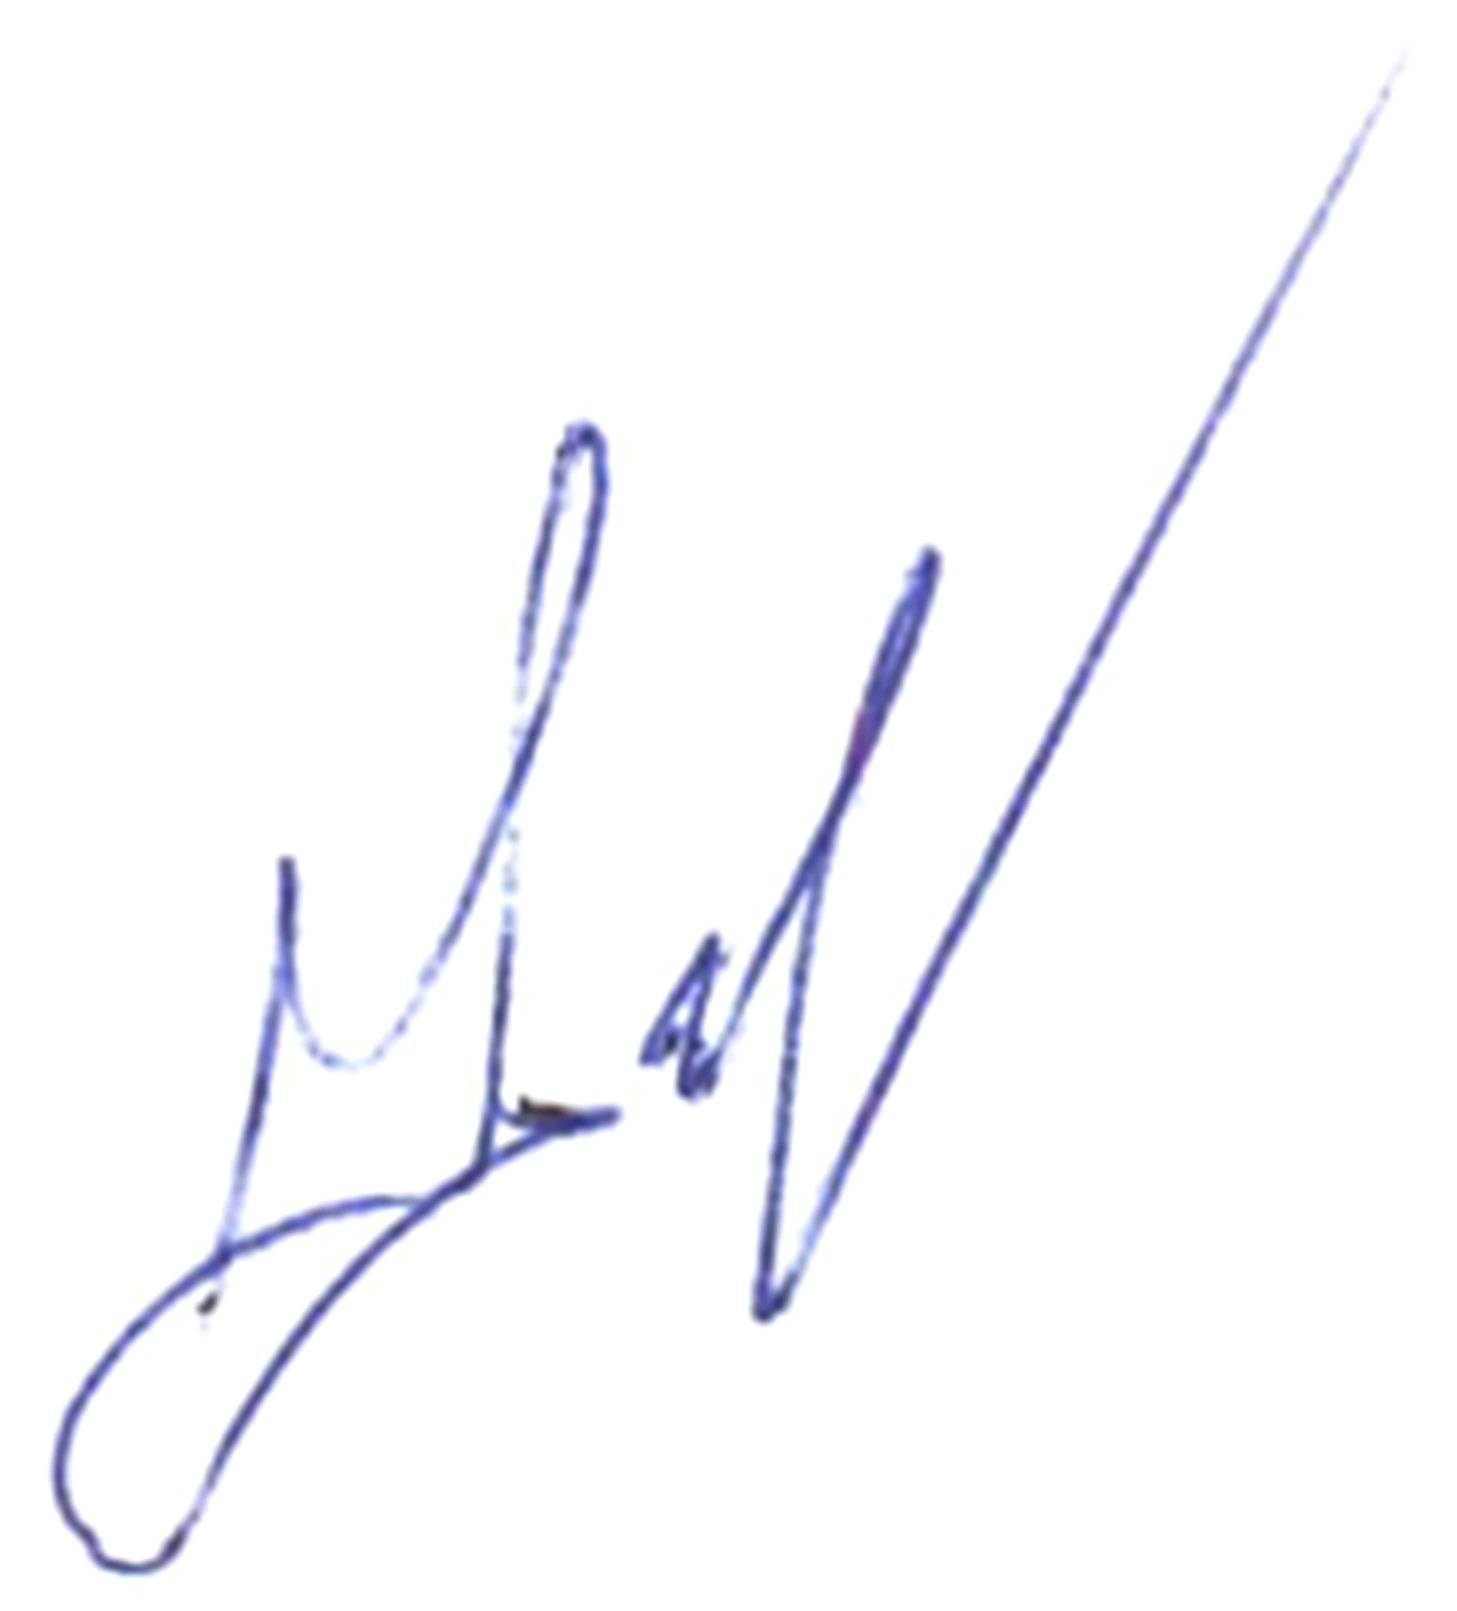
\includegraphics[width=2.3cm]{secretary-signature}
    &
    \defenseSecretaryFio
\end{tabularx} 
           % Титульный лист
% Оглавление (ГОСТ Р 7.0.11-2011, 5.2)
\ifdefmacro{\microtypesetup}{\microtypesetup{protrusion=false}}{} % не рекомендуется применять пакет микротипографики к автоматически генерируемому оглавлению
\tableofcontents*
\ifdefmacro{\microtypesetup}{\microtypesetup{protrusion=true}}{}        % Оглавление
\chapter*{Введение}							% Заголовок
\addcontentsline{toc}{chapter}{Введение}	% Добавляем его в оглавление

\newcommand{\actuality}{}
\newcommand{\aim}{\textbf{Целью}}
\newcommand{\tasks}{\textbf{задачи}}
\newcommand{\defpositions}{\textbf{Основные результаты и
      положения, выносимые на~защиту:}}
\newcommand{\novelty}{\textbf{Научная новизна:}}
\newcommand{\influence}{\textbf{Научная и практическая значимость}}
\newcommand{\reliability}{\textbf{Степень достоверности}}
\newcommand{\probation}{\textbf{Апробация работы.}}
\newcommand{\contribution}{\textbf{Личный вклад.}}
\newcommand{\publications}{\textbf{Публикации.}}

{\actuality} 
% Актуальность - необходимо уметь контролировать рассеяние и поглощение,
% есть невидимость. Добавить 5 ссылок. Актуально сделать маскирующие
% покрытие на основе диэлектриков. 

В последние годы появилось большое количество работ по
нанофотонике~\cite{Tame-quantum-plasmonics-2013,
  Javier-graphene-plasmonics-2014, Khurgin-loss-plasmonics-2015,
  He-tunable-terahertz-graphene-metamaterials-2015,
  Segal-meta-nonlinar-PhC-2015,
  Poddubny-hyperbolic-metamaterials-2013, Kildishev-metasurface-2013}.
Высокая актуальность полученных результатов связана с перспективами их
практического применения и обусловлена стремительным развитием
нанотехнологий, что даёт возможность экспериментальной проверки
предлагаемых идей и подходов. Среди прочих, стоит отметить вопрос о
взаимодействии света с многослойной сферической наночастицей. Он
рассматривается в ряде прикладных задач, таких как: лечение
рака~\cite{Zhang-2010, Hirsch-2003}, различные методы диагностики в
медицине~\cite{Allain-2002}, разработка маскирующих суб-волновых
покрытий для видимого и микроволнового диапазонов~\cite{Qui-2009,
  Semouchkina-2013}, устройства плазмоники~\cite{Martin-2013,
  Alu-2005}, изучение тепловых свойств изоляторов~\cite{Xie-2013},
повышение эффективности солнечных элементов~\cite{Kameya-2011,
  Mann-2011} и так далее. Всё вместе это обуславливает актуальность
настоящей работы, в которой сперва излагается общий принцип,
позволяющий управлять рассеянием и поглощением электромагнитных волн
многослойными сферическими наночастицами, а потом идёт апробация на
частных примерах: минимизация рассеяния от идеально проводящей сферы
(частичная невидимость) и управление поглощением плазмонной частицы
$Si/Ag/Si$.

\underline{\textbf{Основные методы исследования.}}
Теория Ми~\cite{Mie-1908} входит в число основных инструментов применяемых
при анализе задач рассеяния и поглощения плоской электромагнитной
волны сферическими объектами. Эта теория была обобщённа на случай
многослойной сферы с произвольным числом слоёв~\cite{Yang-2003,
  Pena-scattnlay-2009} и доработана в настоящей работе, что позволило
реализовать её в виде комплекса программ для проведения компьютерного
моделирования. Достоинством теории является используемое ей разложение
поля по сферическим векторным гармоникам, что позволяет разделить
вклад в общее поле от электрического и магнитного дипольного
резонанса, а так же вклад резонансов квадруполя
и мультиполей более высокого порядка. Таким образом, становится
возможен анализ спектрального отклика многослойной сферы в зависимости
от её параметров (размеров и показателей преломления слоёв). Например,
в ряде случаев удаётся совместить в спектре рассеяния положение
нескольких резонансов (например, электрических дипольного и
квадрупольного), что создаёт эффект
суперрассеяния~\cite{Fan-2010,Fan-2011}. Аналогичный эффект
суперпоглощения подробно рассмотрен в настоящей работе.


 Как правило, при их решении возникает
необходимость оптимизации дизайна многослойной сферы (радиусов и
материальных параметров составных слоёв), обеспечивающего наилучшие
рабочие характеристики для каждого конкретного случая с учётом
фактических ограничений в предметной области.


\aim\ данной работы является разработка общего подхода к оптимизации
дизайнов многослойных сфер в рамках теории Ми, его последующая
реализация в комплексе компьютерных программ, выявление
закономерностей между дизайном многослойной сферы и её оптическими
свойствами.

Для~достижения поставленной цели необходимо было решить следующие {\tasks}:
\begin{enumerate}
  \item Разработать алгоритм для вычисления рассеяния и поглощения в
    многослойных сферических объектах и реализовать его в комплексе программ.
  \item Выбрать и реализовать алгоритм оптимизации, подходящий для
    работы с произвольными параметрами модели, описываемой обобщённой
    теорией Ми.
  \item Выявить основные закономерности взаимодействия с
    электромагнитной волной сферических маскирующих покрытий на
    основе диэлектриков.
  \item Исследовать эффект суперпоглощения света в многослойных
    сферических наночастицах.
\end{enumerate}



\defpositions
\begin{enumerate}
  \item Получены и реализованны в комплексе программ явные
    реккурентные соотношения для коэффициентов Ми в объёме
    многослойной сферы, выраженные через логарифмические производные
    функций Риккати-Бесселя увеличивающие численную стабильность.  
  
  \item Использование тонкого (размер мишени к размеру покрытия) диэлектриких многослойных покрытий позволяет
    уменьшить рассеяние от идеальное мишени в два раза.
  \item Использовать диэлектрикого порытия для небольшого объекта
    позволяет уменьшить рассеяние в 6 раз.

  \item TODO Использование алгоритма стохастической оптимизации методом
    адаптивной дифференциальной эволюции для решения задачи Ми
    позволяет выявлять семейства дизайнов с заранее заданными
    электромагнитными свойствами.

  \item Защищать цифры (уменьшили в два раза и т.д.). Показано, что
    маскирующие сферические покрытия из диэлектриков могут быть
    сконструированы, используя волноводоподобный эффект.  В этом
    случае при распространении внутри покрытия поле отстает по фазе от
    невозмущённой падающей волны на величину, кратную $2\pi$.
  \item Обнаружено семейство маскирующих сферических порытий из
    диэлектрических изотропных метаматериалов, реализующих эффект
    волнового обтекания.  Для получения заметного эффекта достаточно
    трёх слоёв в покрытии.
  \item В трёхслойных частицах $Si/Ag/Si$ возможно вырождение
    резонансных мультипольных откликов, приводящее к эффекту
    суперпоглощения, когда сечение поглощение оказывается больше, чем
    у bulk частицы. 
  \end{enumerate}

Положения соответствуют пункту 1 паспорта специальности 01.04.05 --
<<Оптика>> (Волновая (физическая) оптика. Интерференция, дифракция,
поляризация, когерентность света) по физико-математическим
наукам (представлены результаты фундаментальных исследований).

%\vspace{5.5em}
\novelty Используем диэлектрики для маскировки, использовать
оптимизация. Есть суперпоглощения.
\begin{enumerate}
  \item Впервые были получены явные реккурентные соотношения для
    коэффициентов Ми в многослойной сфере, выраженные через
    логарифмические производные функций Риккати-Бесселя. 
  \item Впервые метод дифференциальной эволюции был применён
    для изучения маскирующих сферических покрытий, показана высокая
    производительность метода.
  \item Было выполнено оригинальное исследование поглощения света
    наночастицами в режиме вырождения резонансых мультипольных откликов.
\end{enumerate}

\influence. Разработанные аналитические и численные методы для решения
уравнений Максвелла в рамках теории Ми, а так же реализующий их
программный комплекс с использованием стахостической оптимизации
методом дифференциальной эволюции могут быть использованы при
проектировании, оптимизации и анализе (включая анализ предельно
достижимых рабочих характеристик) широкого спектра устройств,
работающих как в оптическом, так и микроволновом диапазоне. Результаты
полученные при изучении поглощени света наночастицами могут быть
использованы при разработке инновационных устройств наноплазмоники,
фотоактивных катализаторов, красителей, поглощающих эмульсий и
аэрозолей.

Результаты диссертационной работы использовались при выполнении
грантов Министерства образования и науки РФ
(проект 11.G34.31.0020, гос. задание 2014/190, задание 3.561.2014/K),
Правительства РФ (грант 074-U01), РФФИ (грант 15-57-45141 ИНД\verb+_+а).


\reliability\ полученных результатов обеспечивается методическим
подходом на каждом этапе работы. Работа оптимизатора была проверена на
наборе стандартных тестовых функций. Аналитические результаты работы
были проверены в системе компьютерной алгебры (IPython). Компьютерная
реализация решения была проверена на наборе тестовых
задач. Аналитические результаты находятся в соответствии с
результатами, полученными другими авторами по теории Ми для случаев
однородной сферы и сферы с одним слоем покрытия.  Случаи большего
числа слоёв в покрытии сравнивался с коммерческими пакетами
моделирования, использующих численные методы конечных разностей во
временной области (Lumerical FDTD), метод конечных элементов (Comsol)
и метод конечных интегралов (CST MWS). Результаты по исследованию
маскирующих покрытий и поглощения света наночастицами находятся в
соответствии с результатами, полученными другими авторами для похожих
систем.

\probation\
Основные результаты работы докладывались~на:
перечисление основных конференций, симпозиумов и~т.\:п.

\contribution\ Автор принимал активное участие \ldots

%\publications\ Основные результаты по теме диссертации изложены в ХХ печатных изданиях~\cite{Sokolov,Gaidaenko,Lermontov,Management},
%Х из которых изданы в журналах, рекомендованных ВАК~\cite{Sokolov,Gaidaenko}, 
%ХХ --- в тезисах докладов~\cite{Lermontov,Management}.
 
\ifthenelse{\equal{\thebibliosel}{0}}{% Встроенная реализация с загрузкой файла через движок bibtex8
    \publications\ Основные результаты по теме диссертации изложены в XX печатных изданиях, 
    X из которых изданы в журналах, рекомендованных ВАК, 
    X "--- в тезисах докладов.%
}{% Реализация пакетом biblatex через движок biber
%Сделана отдельная секция, чтобы не отображались в списке цитированных материалов
    \begin{refsection}%
        \printbibliography[heading=countauthornotvak, env=countauthornotvak, keyword=biblioauthornotvak, section=1]%
        \printbibliography[heading=countauthorvak, env=countauthorvak, keyword=biblioauthorvak, section=1]%
        \printbibliography[heading=countauthorconf, env=countauthorconf, keyword=biblioauthorconf, section=1]%
        \printbibliography[heading=countauthor, env=countauthor, keyword=biblioauthor, section=1]%
        \publications\ Основные результаты по теме диссертации изложены в \arabic{citeauthor} печатных изданиях\nocite{bib1,bib2}, 
        \arabic{citeauthorvak} из которых изданы в журналах, рекомендованных ВАК\nocite{Ladutenko-cloak-2014,Ladutenko-Qabs-2015}, 
        \arabic{citeauthorconf} "--- в тезисах докладов\nocite{DD-14, MW-14}.%
    \end{refsection}
}
% При использовании пакета \verb!biblatex! для автоматического подсчёта
% количества публикаций автора по теме диссертации, необходимо
% их здесь перечислить с использованием команды \verb!\nocite!.
    

 % Характеристика работы по структуре во введении и в автореферате не отличается (ГОСТ Р 7.0.11, пункты 5.3.1 и 9.2.1), потому её загружаем из одного и того же внешнего файла, предварительно задав форму выделения некоторым параметрам

\textbf{Объем и структура работы.} Диссертация состоит из~введения, четырёх глав, заключения и~двух приложений.
%% на случай ошибок оставляю исходный кусок на месте, закомментированным
%Полный объём диссертации составляет  \ref*{TotPages}~страницу с~\totalfigures{}~рисунками и~\totaltables{}~таблицами. Список литературы содержит \total{citenum}~наименований.
%
Полный объём диссертации составляет \formbytotal{TotPages}{страниц}{у}{ы}{} 
с~\formbytotal{totalcount@figure}{рисунк}{ом}{ами}{ами}
и~\formbytotal{totalcount@table}{таблиц}{ей}{ами}{ами}. Список литературы содержит  
\formbytotal{citenum}{наименован}{ие}{ия}{ий}.
    % Введение
\def\slantfrac#1#2{ \hspace{3pt}\!^{#1}\!\!\hspace{1pt}/
  \hspace{2pt}\!\!_{#2}\!\hspace{3pt}
} %Красивые дроби в строчку (например, 1/2)

% \begin{align*}
% f(x) =& x^2\! +3x\! +2 \\
% f(x) =& x^2+3x+2 \\
% f(x) =& x^2\, +3x\, +2 \\
% f(x) =& x^2\: +3x\: +2 \\
% f(x) =& x^2\; +3x\; +2 \\
% f(x) =& x^2\ +3x\ +2 \\
% f(x) =& x^2\quad +3x\quad +2 \\
% f(x) =& x^2\qquad +3x\qquad +2
% \end{align*}

\chapter{Модификация теории Ми для случая многослойной сферы} \label{chapt1}
\section{Современные методы моделирования уравнений Максвелла}
\label{sec:em-methods-intro}
При рассмотрении вопроса о рассеянии и поглощении электромагнитных
волн многослойными сферическими наночастицами в первую очередь
возникает проблема выбора математической модели, которая описывала бы
такую систему.  В настоящее время существует огромное число методов
компьютерного моделирования явлений электромагнетизма достаточно
общего
вида~\cite{Yu-PFDTD-2006,Inan-FDTD-2011,clemson,Bondenson-CEM-2005,Yu-Advanced-FDTD-2011}:
\begin{itemize}
\item метод конечных элементов (finite element method, FEM)
\item метод конечных объёмов во временной области (finite volume
  time-domain, FVTD)
\item метод моментов (method of moments, MoM), обычно реализуемый
  в рамках метода граничных элементов (boundary element method, BEM)
\item метод конечных интегралов (finite integration technique, FIT)
\item метод конечных разностей в временной области (finite difference
  time domain, FDTD)
\item метод конечных разностей в частотной области (finite difference
  frequency domain, FDFD)
\item псевдоспектральный метод во временной области (pseudospectral
  time domain method, PSTD)
\item метод матриц линий передач (transmission line matrix method,
  TLM)
\item приближение дискретных диполей (discrete dipole approximation, DDA)
\end{itemize}
Здесь не упоминаются модификации и усовершенствования этих методов
(иногда существенным образом меняющие исходный алгоритм), как и не
отмечено большое число других методов.  В целом, каждый из методов
можно пытаться классифицировать по следующим параметрам: в основе
лежит интегральная или дифференциальная форма уравнений Максвелла,
метод оперирует данными во временной или в частотной области,
дискретизации подвергается вся модель или только границы её составных
объёмов и т.д.

Сравнение этих методов приводится во многих источниках.
В~\cite{Inan-FDTD-2011} перечисляются такие достоинства метода FDTD,
как малое время разработки работоспособной программы, его простота
для понимания и то, что он работает с уравнениями Максвелла в явном
виде, не привлекая приёмы линейной алгебры, а также его недостатки:
ступенчатая аппроксимация и большая вычислительная сложность.  При
сравнении с методом FVTD отмечается, что последний лучше подходит для
неоднородных объектов, время моделирования сопоставимо с временем
метода FDTD, а основным недостатком является необходимость
дискретизации объёма модели неоднородной сеткой (что в общем случае
является нетривиальной задачей).  Сильные стороны метода FDFD
демонстрируются в случае, когда необходимо получить установившееся
решение для одной частоты.  Особо ярко это проявляется для материалов,
чья зависимость от частоты не может быть формализована простыми
моделями для метода FDTD и для систем с высокодобротным резонансом.
Достоинства FEM аналогичны достоинствам метода FVTD, а основной
недостаток состоит в том, что необходимо решать всю систему уравнений
(она может быть очень большой) для всего объекта моделирования
сразу. Значимость этого недостатка может быть несколько уменьшена за
счёт использования итеративных методов и ряда других техник, связанных
с предварительными преобразованиями используемых матричных систем
уравнений.  PSTD, относящийся к спектральным методам, характеризуется
тем, что применяет разложение (чаще всего Фурье) полей общего решения
модели.  При этом используется значительно менее плотная сетка
дискретизации, что даёт существенный выигрыш в задействованных памяти
и вычислительных ресурсах компьютера.

В книге~\cite{Bondenson-CEM-2005} для выбранного пространственного
размера задачи (3D) приводится вычислительная сложность разных методов
в зависимости от частоты $f$ изучаемого электромагнитного поля.  Для
FDTD число операций растёт как $O(f^4)$, основной недостаток ---
ступенчатая аппроксимация границ, проходящих под углом к направлениям
прямоугольной сетки дискретизации.  FVTD хорошо справляется со
сложными геометриями объектов модели, требует приблизительно такое же
количество вычислительных ресурсов, что и
FDTD, но обладает слабой <<отложенной>> нестабильностью.
Вычислительная сложность FEM растёт как $O(f^4)$ и для частотной, и
для временной области, он более стабилен, чем FVTD.  Для регулярной 3D
сетки дискретизации TLM может быть представлен в форме, эквивалентной
FDTD.  FIT обладает вычислительной сложностью FDTD, но позволяет
использовать произвольные сетки дискретизации с сохранением
стабильности.  Вычислительная сложность MoM зависит от выбранного
метода решения системы уравнений.  Для fast multipole method (FMM) это
$O(f^3)$, а для multilevel fast multipole algorithm (MLFMA) это
$O(f^2\log f)$.

В книге~\cite{Yu-Advanced-FDTD-2011} на одной и той же аппаратной
платформе производилось моделирование общего набора задач с помощью
коммерчески доступного программного обеспечения~(ПО), основанного на разных
(указанных в скобках) методах: HFSS~(FEM), CST MWS~(FIT), GEMS~(FDTD),
FEKO~(MoM). Сравнение результатов расчётов даёт довольно хорошее
совпадение для CST и GEMS, которые решили весь
набор тестовых задач. GEMS оказался быстрее (иногда в несколько раз)
CST и использовал меньшее количество оперативной памяти.

Объектом изучения настоящей работы является сферическая наночастица,
что позволяет применять специализированные методы. Прежде
всего, это теория Ми для многослойной сферы~\cite{Yang-2003} и её
развитие в виде метода Т-матриц (Multiple Sphere
T-Matrix)~\cite{MacKowski-2012}.  По сравнению с более общими методами
применение этой теории позволяет значительно сократить объём
вычислений, необходимый, например, для расчёта сечений рассеяния и
поглощения.  Дополнительным преимуществом теории Ми является
возможность разделять вклады электрических и магнитных мультиполей в
общий электромагнитный отклик частицы.


\section{Теория Ми для многослойной сферы: расчёт ближнего поля}
\label{sec:Mie}

Более 100 лет назад Густав Ми опубликовал свою оригинальную
работу~\cite{Mie-1908} о взаимодействии плоской электромагнитной волны
с однородной сферой.  Изложенная в ней теория впоследствии получила
его имя и в настоящее время входит в число основных инструментов,
применяемых при анализе задач рассеяния и поглощения сферическими
объектами.  Несмотря на более чем вековую историю теории Ми, работы по
её дальнейшему развитию ведутся и в настоящее время~\cite{Suzuki-2008,
  MacKowski-2012, Lerme-2000, Xu-2005, Li-2006, Gogoi-2010,
  Santiago-2011}.  Довольно часто авторы таких работ предоставляют
доступ к своим программам, реализующим новые разработки в этой
области, что позволяет напрямую сравнивать их между собой.  К
сожалению, большая часть таких программ относится к случаю сферы с
одним или несколькими слоями покрытия. Рядом авторов были предложены
математические модели~\cite{Yang-2003, Pena-scattnlay-2009},
позволяющие изучать многослойные сферы с произвольным числом
слоёв~\cite{Sheehan-2013,Selmke-2012}.  Основная сложность при этом
связана с численной реализацией этих моделей.

Рассмотрим рассеяние плоской волны, поляризованной вдоль
координаты~$x$, следуя классическому подходу, изложенному в книге
К.Ф.~Борена и Д.Р.~Хафмена~\cite{Bohren-1983}.  В сферических
координатах такую волну можно записать как:
\begin{equation*}
  \label{eq:bh4.21}
  {\rmfamily \mathbf{E}}_i = E_0 e^{i{\rmfamily k}r\cos\theta}
  {\boldsymbol{\hat{\mathbf{\rmfamily e}}}}_{x}\:,
\end{equation*}
\begin{equation*}
{\boldsymbol{\hat{\mathbf{\rmfamily e}}}}_{x} = \,\sin\theta\, \cos\phi\, 
{\boldsymbol{\hat{\mathbf{\rmfamily e}}}}_{r} 
+\, \cos\theta\, \sin \phi\, {\boldsymbol{\hat{\mathbf{\rmfamily e}}}}_{\theta}
-\, \sin \phi\, {\boldsymbol{\hat{\mathbf{\rmfamily e}}}}_{\phi}\:,
\end{equation*}
где $E_0$ амплитуда падающего поля, а $r,\,\theta,\,\phi$ и
${\boldsymbol{\hat{\mathbf{\rmfamily e}}}}$ --- полярные координаты и единичный вектор для
выбранной системы координат, $k$ волновой вектор падающей волны.
Тогда решение для рассеянного поля выражается в виде разложения в ряд:
\begin{align*}
{\rmfamily \mathbf{E}}_s &=\sum_{n=1}^{\infty} E_n \left( i a_n {\rmfamily
    \mathbf{N}}_{e1n}^{(3)} - b_n{\rmfamily\mathbf{M}_{o1n}^{(3)}} \right)\:,\\
{\rmfamily \mathbf{H}}_s &=\frac{k}{\omega\mu}
 \sum_{n=1}^{\infty} E_n \left( i b_n {\rmfamily
    \mathbf{N}}_{o1n}^{(3)} + a_n{\rmfamily\mathbf{M}_{e1n}^{(3)}} \right)\:,  
\end{align*}
где $E_n=i^nE_0(2n+1)/n(n+1)$, $n$ порядок мультиполя, $E_0$ амплитуда
падающего поля, $a_n$ и $b_n$ коэффициенты разложения, соответствующие
электрическим и магнитным мультиполям, ${\rmfamily \mathbf{N}}_{e1n}^{(j)}$,
${\rmfamily \mathbf{N}}_{o1n}^{(j)}$, ${\rmfamily\mathbf{M}_{o1n}^{(j)}}$ и
${\rmfamily\mathbf{M}_{e1n}^{(j)}}$ сферические векторные гармоники,
выражающиеся через тригонометрические функции, полиномы Лежандра и
сферические функции Бесселя и Ханкеля, $\omega$ частота падающей
волны, $\mu$ магнитная проницаемость в вакууме.  Аналогичным образом
может быть выражено поле внутри $l$-ого слоя стратифицированной
сферы~\cite{Yang-2003}:
\begin{align}
{\rmfamily \mathbf{E}}_l &=\sum_{n=1}^{\infty} E_n \left(
                     c_n^{(l)}{\rmfamily\mathbf{M}}_{o1n}^{(1)}
                     -i d_n^{(l)} {\rmfamily \mathbf{N}}_{e1n}^{(1)}
                     +i a_n^{(l)} {\rmfamily \mathbf{N}}_{e1n}^{(3)}
                     - b_n^{(l)}{\rmfamily\mathbf{M}}_{o1n}^{(3)} 
                     \right)\label{eq:3p1}\:,\\
{\rmfamily \mathbf{H}}_l &=\frac{k_l}{\omega\mu} \sum_{n=1}^{\infty} E_n
                     \left(
                      d_n^{(l)}{\rmfamily\mathbf{M}}_{e1n}^{(1)} 
                     +i c_n^{(l)} {\rmfamily \mathbf{N}}_{o1n}^{(1)} 
                     -i b_n^{(l)} {\rmfamily \mathbf{N}}_{o1n}^{(3)} 
                     - a_n^{(l)}{\rmfamily\mathbf{M}}_{e1n}^{(3)} 
                     \right)\:,\label{eq:3p2}  
\end{align}
где для каждого слоя определены коэффициенты разложения $d_n^{(l)}$ и
$c_n^{(l)}$ электрического и магнитного поля для входящей волны
(направленной к центру частицы) и, аналогично, $a_n^{(l)}$ и
$b_n^{(l)}$ для исходящей волны.  Связь между всеми коэффициентами
разложения можно выразить в виде системы рекуррентных уравнений,
которые получаются из граничных условий на непрерывность
нормальных компонент полей на границе между слоями~\cite{Yang-2003}:

\begin{equation} % \tag{S} % tag - вписывает свой текст
  \label{eq:A2d1}
    % \begin{multlined}
    \begin{alignedat}{2}
d^{(l+1)}_{n}m_{l} \psi^{\prime}_{n}&{\left (m_{l+1} x_{l} \right )}
- a^{(l+1)}_{n} m_{l} \zeta^{\prime}_{n}{\left (m_{l+1} x_{l} \right )}-\\
& - d^{(l)}_{n} m_{l+1} \psi^{\prime}_{n}{\left (m_{l} x_{l} \right )} 
+ a^{(l)}_{n} m_{l+1} \zeta^{\prime}_{n}{\left (m_{l} x_{l} \right )}
= 0\:,
\end{alignedat}
\end{equation}
\begin{equation} % \tag{S} % tag - вписывает свой текст
  \label{eq:A2d2}
\begin{alignedat}{2}
c^{(l+1)}_{n} m_{l} \psi_{n}&{\left (m_{l+1} x_{l} \right )}
  - b^{(l+1)}_{n} m_{l} \zeta_{n}{\left (m_{l+1} x_{l} \right )}-\\
&- c^{(l)}_{n} m_{l+1} \psi_{n}{\left (m_{l} x_{l} \right )} 
+b^{(l)}_{n} m_{l+1} \zeta_{n}{\left (m_{l} x_{l} \right )}  =0\:,
\end{alignedat}
\end{equation}
\begin{equation} % \tag{S} % tag - вписывает свой текст
  \label{eq:A2d3}
\begin{alignedat}{2}
c^{(l+1)}_{n} \psi^{\prime}_{n}&{\left (m_{l+1} x_{l} \right )}
- b^{(l+1)}_{n} \zeta^{\prime}_{n}{\left (m_{l+1} x_{l} \right )}-\\
&- c^{(l)}_{n} \psi^{\prime}_{n}{\left (m_{l} x_{l} \right )} 
+b^{(l)}_{n} \zeta^{\prime}_{n}{\left (m_{l} x_{l} \right )}   =0\:,
\end{alignedat}
\end{equation}
\begin{equation} % \tag{S} % tag - вписывает свой текст
  \label{eq:A2d4}
\begin{alignedat}{2}
 d^{(l+1)}_{n} \psi_{n}&{\left (m_{l+1} x_{l} \right )}
- a^{(l+1)}_{n} \zeta_{n}{\left (m_{l+1} x_{l} \right )}-\\
& - d^{(l)}_{n} \psi_{n}{\left (m_{l} x_{l} \right )} 
+ a^{(l)}_{n} \zeta_{n}{\left (m_{l} x_{l} \right )}   =0\:,
\end{alignedat}
% \end{multlined}
\end{equation}
где $m_l$ показатель преломления в слое, нормированный на показатель
преломления окружающего пространства, $x_l=kr_l$ параметр размера
внешнего радиуса слоя, выраженный через его радиус,
$\psi_{n}(z) = z j_n(z)$ и $\zeta_{n}(z) = z h_n^1(z)$ функции
Риккати-Бесселя, выраженные через сферические функции Бесселя и
Ханкеля.  Из выражений для падающей и рассеянной волны получаются
дополнительные условия на коэффициенты разложения
$c_n^{(L+1)}=d_n^{(L+1)}=1$, $a_n^{(L+1)}=a_n$ и $b_n^{(L+1)}=b_n$,
где $L$ общее число слоёв. Так как у центрального слоя $l=1$ нет
внутренней границы, то $a_n^{(1)}=b_n^{(1)}=0$. Последнее условие
является избыточным для системы
уравнений~(\labelcref{eq:A2d1,eq:A2d2,eq:A2d3,eq:A2d4}), и поэтому оно
было использовано для дополнительной проверки самосогласованности
работы компьютерной программы.  Система
уравнений~(\labelcref{eq:A2d1,eq:A2d2,eq:A2d3,eq:A2d4}) распадается на
две независимых линейных системы и может быть решена явно. После
проведения необходимых алгебраических преобразований были получены
значения коэффициентов разложения в виде обратной рекуррентной
последовательности:
\begin{equation}
\label{eq:6p1}
a^{(l)}_n = \frac
{
    {D^{(1)}_{n}}{\left (m_{l} x_{l} \right )}
    T_1\left (m_{l+1} x_{l} \right )
    +
    T_3\left (m_{l+1} x_{l} \right )
    m_{l}/m_{l+1}
}
{
   \zeta_{n}\left (m_{l} x_{l} \right )
   U\left (m_{l} x_{l} \right )
}\:,
\end{equation}
\begin{equation}
\label{eq:6p2}
b^{(l)}_n = \frac
{
    {D^{(1)}_{n}}{\left (m_{l} x_{l} \right )}
    T_2\left (m_{l+1} x_{l} \right )
    m_{l}/m_{l+1}
    +
    T_4\left (m_{l+1} x_{l} \right )
}
{
   \zeta_{n}\left (m_{l} x_{l} \right )
   U\left (m_{l} x_{l} \right )
}\:,
\end{equation}
\begin{equation}
\label{eq:6p3}
c^{(l)}_n = \frac
{
    {D^{(3)}_{n}}{\left (m_{l} x_{l} \right )}
    T_2\left (m_{l+1} x_{l} \right )
    m_{l}/m_{l+1}
    +
    T_4\left (m_{l+1} x_{l} \right )
}
{
   \psi_{n}\left (m_{l} x_{l} \right )
   U\left (m_{l} x_{l} \right )
}\:,
\end{equation}
\begin{equation}
\label{eq:6p4}
d^{(l)}_n = \frac
{
    {D^{(3)}_{n}}{\left (m_{l} x_{l} \right )}
    T_1\left (m_{l+1} x_{l} \right )
    +
    T_3\left (m_{l+1} x_{l} \right )
    m_{l}/m_{l+1}
}
{
   \psi_{n}\left (m_{l} x_{l} \right )
   U\left (m_{l} x_{l} \right )
}\:,
\end{equation}
используя
\begin{equation*}
  U(z) =    {D^{(1)}_{n}}(z) - {D^{(3)}_{n}}(z)\:,
\end{equation*}
\begin{equation*}
  T_1(z) =   a^{(l+1)}_{n}  \zeta_{n}(z) 
           - d^{(l+1)}_{n}  \psi_{n}(z)\:,
\end{equation*}
\begin{equation*}
  T_2(z) =   b^{(l+1)}_{n}  \zeta_{n}(z) 
           - c^{(l+1)}_{n}  \psi_{n}(z)\:,
\end{equation*}
\begin{equation*}
  T_3(z) =  d^{(l+1)}_{n}  D^{(1)}_{n}(z)  \psi_{n}(z) 
          - a^{(l+1)}_{n}  D^{(3)}_{n}(z)  \zeta_{n} (z)\:,
\end{equation*}
\begin{equation*}
  T_4(z) =  b^{(l+1)}_{n}  D^{(1)}_{n}(z)  \psi_{n}(z) 
          - c^{(l+1)}_{n}  D^{(3)}_{n}(z)  \zeta_{n} (z)\:,
\end{equation*}
где  $D^{(1)}_{n} = \psi^{\prime}_{n}/\psi_{n}$ и
$D^{(3)}_{n} = \zeta^{\prime}_{n}/\zeta_{n}$ логарифмические
производные функций Риккати-Бесселя. Подставляя
(\labelcref{eq:6p1,eq:6p2,eq:6p3,eq:6p4}) в уравнения (\ref{eq:3p1}) и
(\ref{eq:3p2}), можно вычислить величину электрического и магнитного
поля внутри и снаружи многослойной сферы.

С очевидностью, решение системы
уравнений~(\labelcref{eq:A2d1,eq:A2d2,eq:A2d3,eq:A2d4}) может быть
выражено и в виде прямой рекуррентной зависимости. Такое решение было
получено, но после реализации в компьютерной программе проявилась
его плохая численная устойчивость, поэтому в настоящей работе
оно не используется.

При этом возникает дополнительная сложность, связанная с вычислением
сферических векторных гармоник, выражаемых через сферические функции
Бесселя ($j=1$) и Ханкеля ($j=3$) первого рода $z_n^{(j)}$~\cite{Bohren-1983}:
\begin{equation}
  \label{eq:2p1}
 \begin{alignedat}{2}
  {\rmfamily\mathbf{M}}_{o1n}^{(j)} =\cos \phi\,
         \pi_n\!\left(\cos \theta\right)
         z_n^{(j)}\!\left( \rho \right)\,
         {\boldsymbol{\hat{\mathbf{\rmfamily e}}}}_{\theta}   
-\,\sin \phi\,
         \tau_n\!\left(\cos \theta\right)
         z_n^{(j)}\!\left( \rho \right)\,
         &{\boldsymbol{\hat{\mathbf{\rmfamily e}}}}_{\phi}\:,
 \end{alignedat}
\end{equation}
%
\begin{equation}
  %\label{eq:2p2}
 \begin{alignedat}{2}
  {\rmfamily\mathbf{M}}_{e1n}^{(j)} =-\,\sin \phi\,
         \pi_n\!\left(\cos \theta\right)
         z_n^{(j)}\!\left( \rho \right)\,
         {\boldsymbol{\hat{\mathbf{\rmfamily e}}}}_{\theta}   
-\, \cos \phi\,
         \tau_n\!\left(\cos \theta\right)
         z_n^{(j)}\!\left( \rho \right)\,
         &{\boldsymbol{\hat{\mathbf{\rmfamily e}}}}_{\phi}\:,
 \end{alignedat}
\end{equation}
%
\begin{equation}
  %\label{eq:2p3}
 \begin{alignedat}{2}
{\mathbf{N}}_{o1n}^{(j)} = \,{\sin} \phi\,n\!\left(n+1\right)
         {\sin}\theta\,
         \pi_n\!\left({\cos} \theta\right)
         \frac{
               z_n^{(j)}\!\left( \rho \right)
              }{\rho}\,
           &{\boldsymbol{\hat{\mathbf{\mathrm e}}}}_{r}\,+   \\
+\,
{\sin} \phi\,
         \tau_n\!\left({\cos} \theta\right)
         \frac{
            \left[\rho z_n^{(j)}\!\left( \rho \right)\right]^{\prime}
              }{\rho}\,
            &{\boldsymbol{\hat{\mathbf{\mathrm e}}}}_{\theta}\,+   \\
+\,
{\cos} \phi\,
         \pi_n\!\left({\cos} \theta\right)
         \frac{
            \left[\rho z_n^{(j)}\!\left( \rho \right)\right]^{\prime}
              }{\rho}\,
            &{\boldsymbol{\hat{\mathbf{\rmfamily e}}}}_{\phi}\:,
\end{alignedat}
\end{equation}
%
\begin{equation}
  %\label{eq:2p4}
 \begin{alignedat}{2}
{\rmfamily \mathbf{N}}_{e1n}^{(j)} = \,\cos \phi\,n\!\left(n+1\right)
         \sin\theta\,
         \pi_n\!\left(\cos \theta\right)
         \frac{
               z_n^{(j)}\!\left( \rho \right)
              }{\rho}\,
           &{\boldsymbol{\hat{\mathbf{\rmfamily e}}}}_{r} \,+  \\
+\,
\cos \phi\,
         \tau_n\!\left(\cos \theta\right)
         \frac{
            \left[\rho z_n^{(j)}\!\left( \rho \right)\right]^{\prime}
              }{\rho}\,
            &{\boldsymbol{\hat{\mathbf{\rmfamily e}}}}_{\theta} \,+  \\
+\,
\sin \phi\,
         \pi_n\!\left(\cos \theta\right)
         \frac{
            \left[\rho z_n^{(j)}\!\left( \rho \right)\right]^{\prime}
              }{\rho}\,
            &{\boldsymbol{\hat{\mathbf{\rmfamily e}}}}_{\phi}\:,
\end{alignedat}
\end{equation}
где обезразмеренное расстояние до центра сферы $\rho=kr$, а угловые
функции
\begin{equation*}
  \label{eq:bh4.46}
  \pi_n=\frac{P_n^1}{\cos\theta} \qquad \mbox{и} \qquad \tau_n = \frac{dP_n^1}{d\theta}
\end{equation*}
выражены через функцию Лежандра $P_n^m$, которая
задаётся через производную полинома Лежандра $P_n$ в виде
\begin{equation*}
  \label{eq:bh4.25}
  P_n^m\left(\mu\right)=\left(1-\mu^2\right)^{m/2}\frac{d^{\,m}P_n(\mu)}{d\mu^m}\:,
\end{equation*}
где $\mu = \cos\theta$. Чтобы рассчитать значения угловых функций,
необходимо воспользоваться рекуррентными
соотношениями~\cite{Wiscombe-1980}
\begin{equation}
  \label{eq:bh4.47a}
  \pi_0 = 0, \qquad \pi_1 = 1, \qquad
  \pi_n = \frac{2n-1}{n-1}\cos\theta\,\pi_{n-1} - \frac{n}{n-1}\pi_{n-2}\:,
\end{equation}
\begin{equation}
  \label{eq:bh4.47b}
  \tau_n = n\cos\theta\,\pi_{n} + (n+1)\pi_{n-1}\:,
\end{equation}
доказавшими свою численную устойчивость.  Таким образом, основную
сложность при вычислении значений сферических векторных гармоник
представляет суммирование рядов, выражающих сферические функции
Бесселя.  Плохая сходимость таких рядов особенно заметна в случае
комплексного аргумента с большой мнимой частью.  Для решения этой
проблемы в настоящей главе предлагается следующий вид сферических
векторных гармоник:
\begin{equation}
  \label{eq:2p1mod}
 \begin{alignedat}{2}
  {\rmfamily\mathbf{M}}_{o1n}^{(j)} =\cos \phi\,
         \pi_n\!\left(\cos \theta\right)
         \frac{r_n^{(j)}\!\left( \rho \right)}{\rho}\,
         {\boldsymbol{\hat{\mathbf{\rmfamily e}}}}_{\theta}   
-\,\sin \phi\,
         \tau_n\!\left(\cos \theta\right)
         \frac{r_n^{(j)}\!\left( \rho \right)}{\rho}\,
         &{\boldsymbol{\hat{\mathbf{\rmfamily e}}}}_{\phi}\:,
 \end{alignedat}
\end{equation}
%
\begin{equation}
  %\label{eq:2p2}
 \begin{alignedat}{2}
  {\rmfamily\mathbf{M}}_{e1n}^{(j)} =-\,\sin \phi\,
         \pi_n\!\left(\cos \theta\right)
         \frac{r_n^{(j)}\!\left( \rho \right)}{\rho}\,
         {\boldsymbol{\hat{\mathbf{\rmfamily e}}}}_{\theta}   
-\, \cos \phi\,
         \tau_n\!\left(\cos \theta\right)
         \frac{r_n^{(j)}\!\left( \rho \right)}{\rho}\,
         &{\boldsymbol{\hat{\mathbf{\rmfamily e}}}}_{\phi}\:,
 \end{alignedat}
\end{equation}
%
\begin{equation}
  %\label{eq:2p3}
 \begin{alignedat}{2}
{\rmfamily \mathbf{N}}_{o1n}^{(j)} = \,\sin \phi\,n\!\left(n+1\right)
         \sin\theta\,
         \pi_n\!\left(\cos \theta\right)
         \frac{
           r_n^{(j)}\!\left( \rho \right)
              }{\rho^2}\,
           &{\boldsymbol{\hat{\mathbf{\rmfamily e}}}}_{r}\,+   \\
+\,
\sin \phi\,
         \tau_n\!\left(\cos \theta\right)
         \frac{
           D_n^{(j)}\!(\rho) r_n^{(j)}\!(\rho)
              }{\rho}\,
            &{\boldsymbol{\hat{\mathbf{\rmfamily e}}}}_{\theta}\,+   \\
+\,
\cos \phi\,
         \pi_n\!\left(\cos \theta\right)
         \frac{
           D_n^{(j)}\!(\rho) r_n^{(j)}\!(\rho)
              }{\rho}\,
            &{\boldsymbol{\hat{\mathbf{\rmfamily e}}}}_{\phi}\:,
\end{alignedat}
\end{equation}
%
\begin{equation}
  %\label{eq:2p4}
 \begin{alignedat}{2}
{\rmfamily \mathbf{N}}_{e1n}^{(j)} = \,\cos \phi\,n\!\left(n+1\right)
         \sin\theta\,
         \pi_n\!\left(\cos \theta\right)
         \frac{
               r_n^{(j)}\!\left( \rho^2 \right)
              }{\rho}\,
           &{\boldsymbol{\hat{\mathbf{\rmfamily e}}}}_{r}\,+   \\
+\,
\cos \phi\,
         \tau_n\!\left(\cos \theta\right)
         \frac{
           D_n^{(j)}\!(\rho) r_n^{(j)}\!(\rho)
              }{\rho}\,
            &{\boldsymbol{\hat{\mathbf{\rmfamily e}}}}_{\theta}\,+   \\
+\,
\sin \phi\,
         \pi_n\!\left(\cos \theta\right)
         \frac{
           D_n^{(j)}\!(\rho) r_n^{(j)}\!(\rho)
              }{\rho}\,
            &{\boldsymbol{\hat{\mathbf{\rmfamily e}}}}_{\phi}\:,
\end{alignedat}
\end{equation}
где используются функции Риккати-Бесселя $r_n^{(1)} = \psi_n$ и
$r_n^{(3)} = \zeta_n$ и их логарифмические производные, благодаря чему
автору удалось заметно увеличить численную устойчивость
расчёта по теории Ми. Дело в том, что функции Риккати-Бесселя могут быть записаны
в виде рекуррентных соотношений с хорошей сходимостью для более
широкого диапазона аргументов~\cite{Wiscombe-1980,Mackowski-1990} по
сравнению со сферическими функциями Бесселя следующим образом:
\begin{equation*}
  \label{eq:pena16a}
  D_{N_{\scalebox{0.65}{\rmfamily max}}}^{(1)}(z) = 0 + i0\:,
\end{equation*}
\begin{equation*}
  \label{eq:pena16b}
  D_{n-1}^{(1)}(z) = \frac{n}{z} -\frac{1}{D_n^{(1)}(z)+n/z}\:,\quad n=N_{\max}, \ldots, 0\:,
\end{equation*}
где выражение для количества членов рекурсии $N_{\rmfamily nmax}$ было
предложено в работе~\cite{Wiscombe-1980}:
\begin{equation*}
  N_{\max} = \max\left(N_{\rmfamily stop}, \left|m_lx_l\right|,
    \left|m_lx_{l-1}\right|
\right) + 15\:, \quad l=1,2,\ldots,L\:,
\end{equation*}
\begin{equation*}
\label{eq:pena17}
  N_{\rmfamily stop}=
\begin{cases}
x_L+4x_L^{\slantfrac{1}{3}}+1\:,\quad & 0.02\leqslant x_L<8\:,\\
x_L+4.05x_L^{\slantfrac{1}{3}}+2\:,\quad & 8\leqslant x_L<4\,200\:,\\
x_L+4x_L^{\slantfrac{1}{3}}+2\:,\quad & 4\,200\leqslant x_L<20\,000\:.\\
\end{cases}
\end{equation*}
В работе~\cite{Mackowski-1990} была показана численная устойчивость
следующего метода для вычисления $D_n^{(3)}$:
\begin{equation*}
  \label{eq:pena18a}
  \psi_0(z)\zeta_0(z)=\frac{1}{2}
\left[
1-(\cos\,2a+i\,\sin\,2a)exp(-2b)
\right],
\end{equation*}
\begin{equation*}
  \label{eq:pena18b}
D_0^{(3)} = i\:,
\end{equation*}
\begin{equation*}
  \label{eq:pena18c}
  \psi_n(z)\zeta_n(z)=   \psi_{n-1}(z)\zeta_{n-1}(z)
\left[
\frac{n}{z}-D_{n-1}^{(1)}(z)
\right]
\left[
\frac{n}{z}-D_{n-1}^{(1)}(z)
\right],
\end{equation*}
\begin{equation*}
  \label{eq:pena18d}
D_n^{(3)}(z) = D_n^{(1)}(z)+\frac{i}{\psi_n(z)\zeta_n(z)}\:,\quad
n=1,\ldots, N_{\max}\:,
\end{equation*}
где $z=a+ib$. Функции Риккати-Бесселя задаются следующими
выражениями~\cite{Wiscombe-1980,Mackowski-1990}:
\begin{equation*}
  \label{eq:pena20a}
  \psi_0(z) = \sin(z)\:,
\end{equation*}
\begin{equation*}
  \label{eq:pena20b}
\psi_n(z) = \psi_{n-1}(z)
\left[
\frac{n}{z}-D_{n-1}^{(1)}(z)
\right], \quad n=1,\ldots, N_{\max}\:,
\end{equation*}
\begin{equation*}
  \label{eq:pena21a}
\zeta_0(z) = \sin(z) - i\,\cos(z)\:,
\end{equation*}
\begin{equation*}
  \label{eq:pena21b}
\zeta_n(z) = \zeta_{n-1}(z)
\left[
\frac{n}{z}-D_{n-1}^{(3)}(z)
\right], \quad n=1,\ldots, N_{\max}\:.
\end{equation*}
Таким образом, в настоящем разделе предложен математический аппарат,
позволяющий вычислять локальные поля в случае падения плоской
электромагнитной волны на сферическую многослойную
частицу. Разработанный метод отличается высокой надёжностью и
устойчивостью в широком диапазоне входных параметров, что, среди
прочих факторов, вызвано использованием оригинального вида сферических
векторных гармоник в представлении через логарифмические производные
функций Риккати-Бесселя.


\section{Компьютерная реализация алгоритма расчёта по теории Ми}
\label{sec:code}

% \subsection{Выбор алгоритма, языка программирования, оптимизация
% быстродействия}

Для проведения расчётов с использованием выражений, полученных в
разделе~\ref{sec:Mie}, наиболее рациональным является применение
компьютера.  Для этого необходимо разработать новую или модифицировать
ранее созданную компьютерную программу. Второй вариант, как менее
трудоёмкий, является предпочтительным.  При этом необходимо принимать
во внимание целый ряд факторов:
\begin{itemize}
\item Функциональность уже готовых программ.
\item Возможности по их модификации, которые прежде всего определяются
  доступностью исходного текста программы и используемыми языками
  программирования.
\item Количество и качество документации, описывающее работу
  программы, наличие возможности получить консультацию у авторов,
  простота её использования.
\item Производительность.
\end{itemize}

В сети Интернет~\cite{scattport,wiki-mie-codes} и в
литературе~\cite{Wriedt-2009} можно найти описания десятков программ,
выполняющих расчёты по теории Ми.  Довольно часто они базируются на
коде BHMIE, описанном в книге К.Ф.~Борена и
Д.Р.~Хафмена~\cite{Bohren-1983}.  Заслуженное признание получил код
MIEV0~\cite{Wiscombe-1980}, основанный на специальном
алгоритме~\cite{Lentz-76} для представления сферических функций
Бесселя. Дальнейшее развитие метода дало возможность моделировать
агрегаты из нескольких сферических частиц~\cite{Mackowski-96,Xu-95}.

Ряд работ описывает взаимодействие света с многослойной
сферой~\cite{Kai-94,Wu-97, Bhandari-85}.  Наибольшей численной
устойчивостью, насколько об этом можно судить из обзора литературы,
обладает алгоритм, предложенный в 2003 году W.~Yang~\cite{Yang-2003} и
реализованный O.~Pe\~{n}a-Rodr\'{i}guez в 2009
году~\cite{Pena-scattnlay-2009} в виде публично доступной программы.
Именно эта реализация и была выбрана в качестве основы для программы,
разрабатываемой в рамках настоящей диссертации, как наиболее полно
соответствующая изложенным выше требованиям.  Тем не менее, для
достижения цели, поставленной в диссертации, оказалась необходима
существенная переработка исходной программы.

Прежде всего это касалось ряда технических моментов. Так как программа
была написана на языке программирования Си, то в ней использовалось
прямое выделение памяти для хранения данных.  Применение
родственного языка Си\texttt{++} позволило перейти к использованию
динамических массивов, что заметно упростило
программу и сделало более эффективным её эксплуатацию в качестве
внешней библиотеки.

Использование объектно-ориентированной парадигмы программирования
позволило автоматизировать ряд рутинных операций, тем самым избавив
конечного пользователя от их выполнения, сохранив при этом достаточно
чёткую структуру программы.  Прежде всего это касается проверки
корректности вводимых параметров модели (толщины слоёв должны быть
положительными, для каждого слоя требуется задать толщину и показатель
преломления, было реализовано большое число прочих проверок). Кроме
того, появилась возможность задания параметров модели в размерных
величинах, а перевод в безразмерные величины происходит внутри
программы. Всё это уменьшает возможность ошибок из-за человеческого
фактора.

Следующий момент связан с выполнением операций над комплексными
числами.  В оригинальной программе для выполнения арифметических
действий (умножения, деления, вычитания и так далее) определялись
явные функции вида \verb+Cmul(a,b)+, \verb+Cdiv(a,b)+,
\verb+Csub(a,b)+, где \verb+a+ и \verb+b+ переменные, содержащие
значение комплексного числа.  Переход на использование языка
программирования Си\texttt{++} позволил воспользоваться возможностями
стандартной библиотеки \verb+std::complex+, а запись упомянутых
арифметических операций приобрела естественный вид, например,
\verb!a*b!, \verb!a/b!, \verb!a-b! и тому подобное.  Это значительно
упрощает ввод в текст вычислительной программы выражений, полученных
при аналитическом анализе проблемы.

Важной характеристикой работы любой программы является её
быстродействие, в этом случае существенное значение оказывает выбор
языка программирования.  С момента своего появления (вторая половина
1950-х) и вплоть до начала 2000-х годов лучшим языком для научных и
инженерных вычислений было принято считать Фортран, специально для
этих целей и разработанный. Весомым плюсом языка является наличие
огромного количества свободно распространяющихся библиотек
математических операций. В то же время достаточно широкое
распространение получил язык Си, став одним из самых используемых
языков программирования, а также заложив основу синтаксиса для других
языков (например, Си\texttt{++}).  К недостаткам Си можно было отнести
лишь недостаточно высокую производительность, из-за чего аналоги
программ на Фортране были быстрее вплоть до десятка
раз~\cite{Veldhuizen-1997}. Тем не менее, улучшение оптимизации кода
компиляторами Cи/Cи\texttt{++}, рост числа специализированных
библиотек, популяризация языков Си и Си\texttt{++}, связанная с
распространением операционной системы Unix (и с сопутствующим ростом
количества доступных качественных учебных материалов по языку и
специальной литературы, приведшей, как следствие, к увеличению числа
высококвалифицированных специалистов, использующих эти языки для
решения широкого спектра задач), позволили значительно повысить среднюю
эффективность вычислительных программ на языках Си и Си\texttt{++},
достигнув паритета с аналогичными программами на
Фортране~\cite{Veldhuizen-1997,Markovich-FDTD-2013}.  Это означает,
что дальнейший рост быстродействия ограничен аппаратными возможностями
компьютера.  Кроме того, к преимуществам языков Си и Си\texttt{++}
относится значительно меньшая стоимость разработки и развития сложных
проектов.  Всё вместе это позволяет сделать вывод о том, что в
настоящее время Си\texttt{++} является наилучшим выбором языка для
программирования требовательных к вычислениям задач.

Само по себе написание программы на наиболее подходящем для конечной
задачи языке программирования не гарантирует достижения наилучшего
быстродействия.  Стандартной процедурой для увеличения быстродействия
является временн\'ое профилирование программы, которое позволяет
выявить места, требующие больше всего вычислительных ресурсов.  Далее
оптимизация производится только для подобных мест, так как остальные
части программы не оказывают существенного влияния на общее время
выполнения.  При доработке настоящей программы было выявлено несколько
таких мест, среди которых особо хотелось отметить вычисление
уравнений~\ref{eq:bh4.47a} и~\ref{eq:bh4.47b}.  Для них наиболее
трудоёмкой частью с вычислительной точки зрения них оказалась задача
нахождения косинуса угла. Так как значение угла не меняется внутри
цикла рекурсии, то предварительное вычисление вне цикла дало большую
часть ускорения работы программы для ряда тестовых примеров.

В итоге программа для проведения вычислений по теории Ми была полностью
переработана, она получила возможность расчёта полей, оптимизация уже
существовавших алгоритмических решений позволила сократить время
выполнения в 2.2 раза.  Все описанные доработки были с благодарностью
приняты оригинальным автором программы Ovidio Pe\~{n}a-Rodr\'{i}guez и
в полном объёме добавлены в исходной код
программы~\cite{Scattnlay-web}.

Предложенное представление сферических векторных гармоник через
логарифмические производные функций Риккати-Бесселя позволило
значительно расширить границы численной устойчивости метода.  Для
дальнейшего развития программы расчёта начаты работы по использованию
библиотек контролируемой точности вычислений (arbitrary-precision
arithmetic).  Первые результаты на этом пути показали практическую
реализуемость подобного решения.

% \subsection{Верификация работы на тестовых примерах}

Важным этапом работ была верификация программы на нескольких
тестовых примерах:
\begin{itemize}
\item Однородная сфера, что является предельным случаем многослойной
  сферы с одним слоем $L=1$.
\item Сфера с покрытием $L=2$. Этот и предыдущий примеры позволяют
  провести сравнения с хорошо изученными случаями, для которых
  известно аналитическое решение.
\item Трёхслойная наночастица $Si/Ag/Si$. В этом случае сравнение
  будет проводиться с результатами полноволнового моделирования
  методом FDTD, которое выполнялось с использованием коммерческого ПО.
\item Многослойное маскирующее покрытие, сравнение выполняется с
  коммерческим ПО CST MWS, использующим для моделирования в частотной
  области метод конечных элементов.
\end{itemize}

В качестве первого теста был взят пример из работы М.В.~Башевого
и~др.~\cite{Bashevoy-2005}, в которой рассматривалось образование
нановихрей в наночастице золота. 
\begin{figure}[p]
  \begin{minipage}[ht]{0.99\linewidth}
    \centering{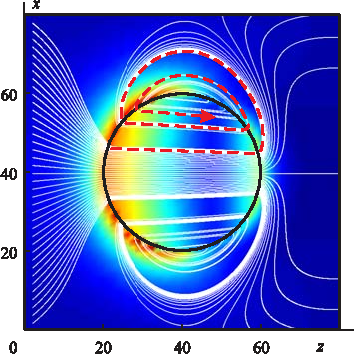
\includegraphics[width=0.59\linewidth]{bashevoj-oe-13-21-8372-fig}}
  \end{minipage}\\
  \vfill
  \begin{minipage}[ht]{0.99\linewidth}
    \centering{а)}
  \end{minipage}\\
  \vfill
  \begin{minipage}[ht]{0.99\linewidth}
    \centering{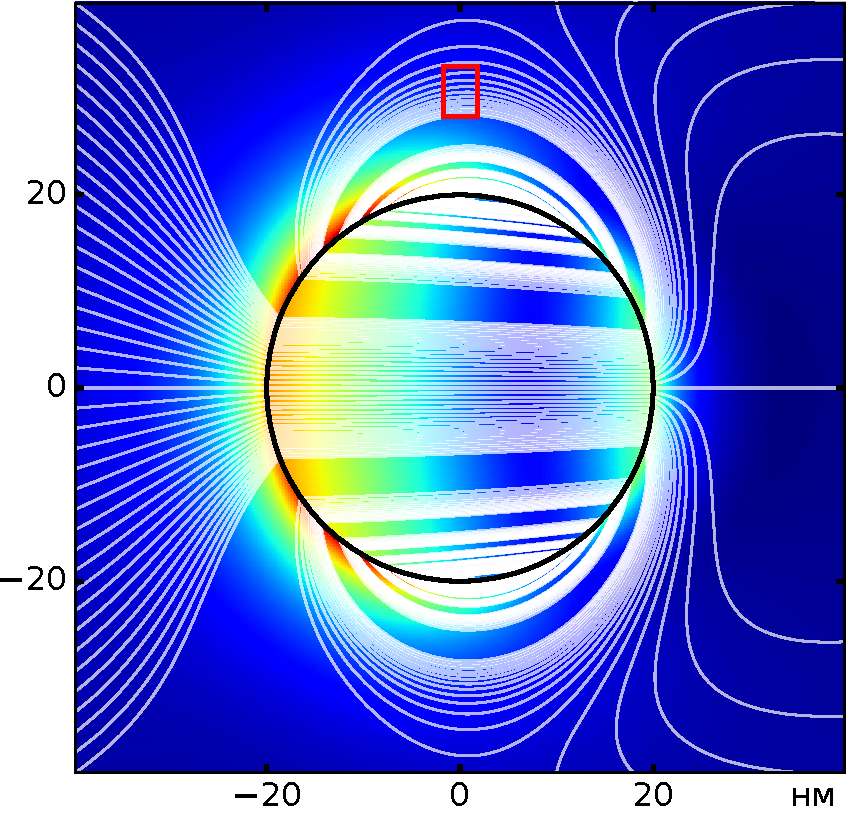
\includegraphics[width=0.59\linewidth]{bulk-Ag-flow-R20-XZ-Pabs-mark}
    }
  \end{minipage}\\
  \begin{minipage}[ht]{0.99\linewidth}
    \centering{б)}
  \end{minipage}
  \caption{Золотая сфера $r=20$~нм при облучении светом с длиной волны
    $\lambda=354$~нм, (a) результат из работы М.В.~Башевого
    и~др.~\cite{Bashevoy-2005}, (б) результат расчёта ближнего поля по
    выражениям из раздела~\ref{sec:Mie}. Цвет меняется от синего к
    красному что характеризует рост величины вектора Пойнтинга, касательная к
    белым линиям --- его направление. Волна падает слева
    направо.\label{img:vortex}}
\end{figure}
Расчёт полей при этом проводился с помощью метода конечных элементов в
программе Comsol~\cite{Comsol-web}. Так как дискретизация модели производится с помощью
неупорядоченной сетки, то нарушается собственная симметрия системы,
что хорошо видно на перепечатанном из оригинальной работы
рисунке~\ref{img:vortex}(а).  В области больших значений амплитуды
вектора Пойнтинга в верхней половине на границе сферы амплитуда
меняется достаточно плавно, а в нижней наблюдается несколько областей
с локальными максимумами.

На рисунке~\ref{img:vortex}(б) его верхняя и нижняя половины
зеркально-симметричны, как и стоит ожидать от аналитического
расчёта. В целом стоит отметить хорошее совпадение результатов
полноволнового моделирования в коммерческом ПО с результатами,
полученными в настоящей главе.  Кроме уже отмеченных небольших различий
в амплитуде вектора Пойнтинга заметны и сопутствующие различия в
линиях потока энергии. В работе М.В.~Башевого
и~др.~\cite{Bashevoy-2005} указано, что эти линии были получены в
результате численного решения уравнения
\begin{equation*}
  \frac{d\mathbf{\rmfamily A}}{dt}=\mathbf{\rmfamily S}(\mathbf{\rmfamily A})\:,
\end{equation*}
где $\,\mathbf{\rmfamily A}(t)$ поле вектора Пойнтинга
$\,\mathbf{\rmfamily S}=\left[\mathbf{\rmfamily
    E}\times\mathbf{\rmfamily H}\right]$, $\,t$ ---~координата вдоль
линии.  При таком подходе положение линий потока энергии может быть
дополнительно искажено из-за ошибок в расчёте поля
$\mathbf{\rmfamily A}$. Это становится особенно заметно в структурах с
резкими изменениями амплитуды поля, например, на границе сферы, или
при наличии вихрей потока энергии, где протяжённость этих линий
значительно увеличивается.

Для того чтобы увеличить точность построения, в настоящей работе был
предложен следующий алгоритм, который позволяет контролировать
возникающую ошибку. Линия потока энергии строится из некой начальной
точки, как упорядоченная последовательность прямых отрезков, где
каждый последующий начинается в конце предыдущего. Направление
отрезка задаётся вещественной частью среднего значения за период
колебаний вектора Пойнтинга
\begin{equation*}
  \left\langle\mathbf{\rmfamily S}\right\rangle = \frac{1}{2}
  \left[\mathbf{\rmfamily E}\times\mathbf{\rmfamily H}^*\right]\:.
\end{equation*}
Длина текущего отрезка зависит от направления вектора
$\operatorname{\mathbb{R}e}\left\langle\mathbf{\rmfamily S}\right\rangle$ в
его конечной точке. Если его направление отличается от текущего
на значение большее, чем пороговый угол (эта величина является
параметром построения и в настоящей работе, если не указано иное, была
принята равной одному градусу), то длина отрезка уменьшается в два
раза, и расчёт производится заново до тех пор, пока не будет найдено
удовлетворительное значение длины. Перед расчётом
следующего отрезка используемая длина увеличивается в два раза, что
позволяет быстро достичь максимально возможного значения для
заданной точности построения.

При прохождении через границу раздела двух сред непрерывной является
только нормальная компонента вектора Пойнтинга. Поэтому, если отрезок
пересекает эту границу, то уменьшение его длины практически не влияет
на направление следующего отрезка. Чтобы избежать бесконечного
уменьшения длины в такой ситуации, был задан второй параметр
построения ---~минимальная длина отрезка.  В настоящей работе, если не
указано иное, это значение бралось в $2\,000$ раз меньше радиуса
внутреннего слоя многослойной сферы, что позволяет с контролируемой
точностью совмещать изломы линии потока энергии с границами
раздела. При этом значительно сокращается необходимый объём вычислений
для построения областей с небольшой кривизной линий потока энергии.

Результат работы предложенного алгоритма для построения линий потока
энергии можно оценить на рисунке~\ref{img:vortex}(б).  По сравнению с
рисунком~\ref{img:vortex}(а) внутри и вблизи частицы удалось получить
более плавное изменение расстояния между линиями потока энергии,
стартовые точки для которых были расположены через равные интервалы на
некотором отдалении от рассматриваемой сферы.  Уменьшая значение параметров
построения (пороговый угол и минимальная длина отрезка), несложно
проверить его стабильность.
\begin{figure}[t] {\centering
  \begin{minipage}[ht]{0.49\linewidth}        
    \centering{
\includegraphics[width=0.6\linewidth]{bulk-Ag-flow-R20-XZ-Pabs-crop} }
  \end{minipage}
  \begin{minipage}[ht]{0.49\linewidth}
    \centering{
\includegraphics[width=0.6\linewidth]{bulk-Ag-flow-R20-XZ-Pabs-fine-crop} }
  \end{minipage}
}\\
{\centering
  \begin{minipage}[ht]{0.49\linewidth}
    \centering{а)}
  \end{minipage}
  \begin{minipage}[ht]{0.49\linewidth}
    \centering{б)}
  \end{minipage}
}
\caption{Фрагмент из области на рисунке~\ref{img:vortex}(б),
  выделенный красным прямоугольником. Случай (а) исходных параметров
  для построения линий потока энергии, (б) пороговый угол уменьшен в 2
  раза, минимальная длина отрезка в 10 раз.\label{img:vortex-crop}}
\end{figure}
Для этого на рисунке~\ref{img:vortex-crop}(а) было построено
увеличенное изображение фрагмента рисунка~\ref{img:vortex}(б) из
области, выделенной красным прямоугольником. На
рисунке~\ref{img:vortex-crop}(б) были изменены параметры построения
линий потока энергии: пороговый угол уменьшен в 2 раза, минимальная
длина отрезка уменьшена в 10 раз. Видно, что хотя общий характер
картины не изменился, тем не менее есть несколько отличий. Все линии
немного сместились (приблизительно на ширину изображаемой линии),
более важное изменение касается расстояния между ними. На
рисунке~\ref{img:vortex-crop}(а) оно убывает неравномерно, например,
для нижних четырёх линий расстояние между парой вторая/третья
больше, чем между парами линий первая/вторая и третья/четвёртая. У
такого поведения нет физического обоснования, оно вызвано небольшой
ошибкой при построении линий потока энергии.  После изменения
параметров построения в сторону обеспечения большей точности ситуация
исправилась, визуально расстояние между линиями на
рисунке~\ref{img:vortex}(б) изменяется монотонно при их последовательном
переборе по вертикали.
 
Для сравнения случая двухслойных структур была выбрана программа
BHFIELD~\cite{Suzuki-2008,Suzuki-2013}, доступная в
сети Интернет.  Это позволило задавать идентичные параметры
моделирования для BHFIELD и программы, разработанной в настоящей
главе. Моделировалась диэлектрическая частица с радиусом $R_1=50$~нм и
показателем преломления $n_1=1.53413$, покрытая 10~нм слоем серебра (в
результате внешний радиус частицы $R_2=60$~нм) с показателем
преломления $n_2=0.565838+i7.23262$ (что соответствует длине волны
$\lambda = 1\,064$~нм), расположенная в диэлектрической матрице с
показателем преломления $n_m=1.3205$.  Результаты, полученные в версии
BHFIELD для двойной точности вычислений, полностью соответствуют
результатам программы, разработанной в настоящей главе.

Случай сферы, состоящей из трёх слоёв, проверялся с использованием
коммерческого пакета моделирования Lumerical
FDTD~\cite{Lumerical-web}. Рассматривалась система $Si/Ag/Si$ с
радиусами $r_l=\{17.74, 41.05, 64\}$~нм, длина волны падающего
излучения $\lambda = 800$~нм, при этом относительная диэлектрическая
проницаемость бралась равной $\varepsilon_{Si} = 13.64 + i 0.047$ для
кремния и $\varepsilon_{Ag} = -28.05 + i 1.525$ для серебра.
Результаты расчёта методом FDTD и по теории Ми представлены на
рисунке~\ref{img:fdtd}.
\begin{figure}[p] 
  \begin{minipage}[ht]{0.99\linewidth}
    \centering{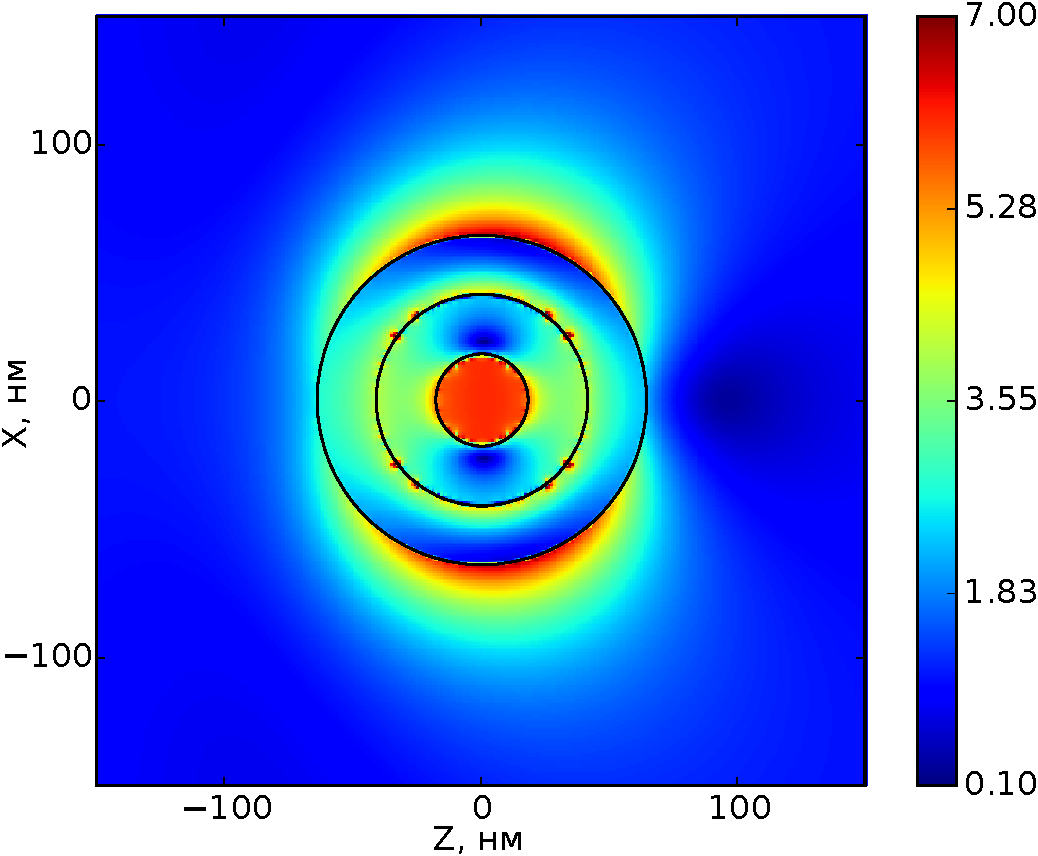
\includegraphics[width=0.67\linewidth]{lumerical-R64-XZ-Eabs}}
  \end{minipage}\\
  \vfill
  \begin{minipage}[ht]{0.99\linewidth}
    \centering{а)}
  \end{minipage}\\
  \vfill
  \begin{minipage}[ht]{0.99\linewidth}
    \centering{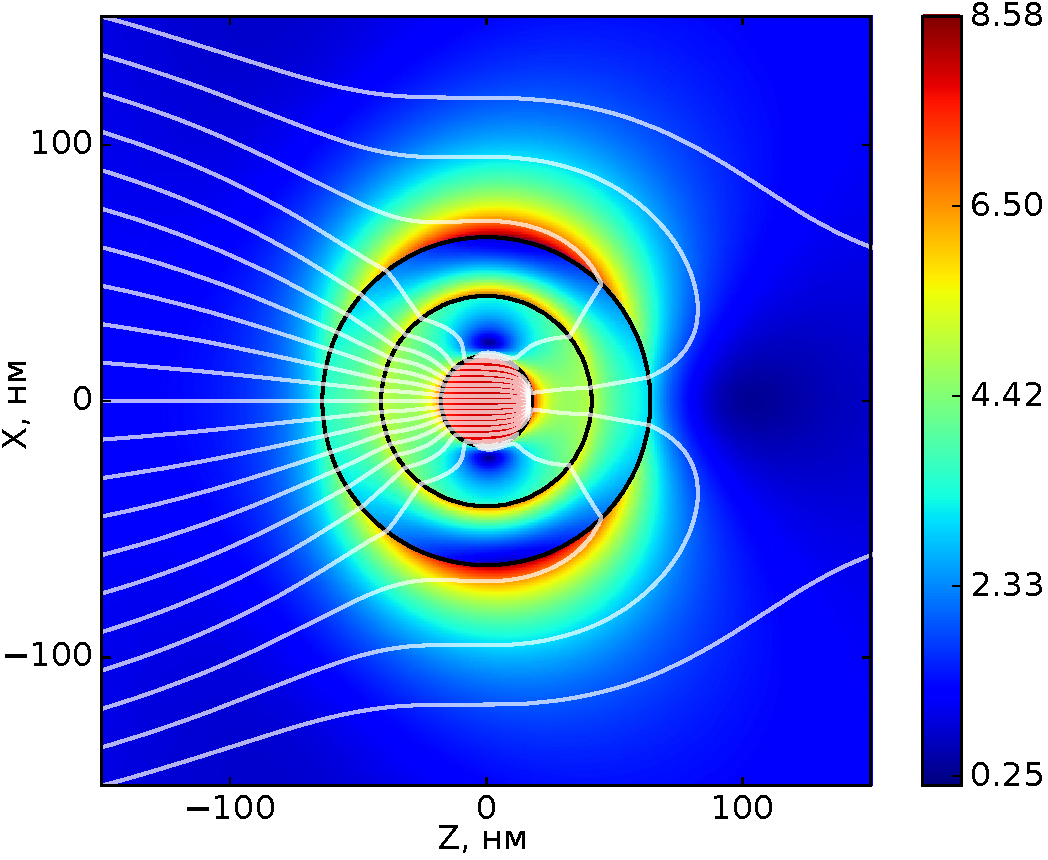
\includegraphics[width=0.67\linewidth]{SiAgSi-absorber-flow-R64-XZ-Eabs}
    }
  \end{minipage}\\
  \vfill
  \begin{minipage}[ht]{0.99\linewidth}
    \centering{б)}
  \end{minipage}
  \caption{Картина ближнего поля для частицы $Si/Ag/Si$ с общим
    радиусом 64~нм. (a) Результат моделирования в Lumerical FDTD, (б)
    результат расчёта ближнего поля по выражениям из
    раздела~\ref{sec:Mie}. Цвет характеризует величину электрического
    поля $|E|/|E_0|$, касательная к белым линиям --- направление
    вектора Пойнтинга. Волна падает слева направо.\label{img:fdtd}}
\end{figure}

В целом картина ближнего поля в обоих случаях оказалась довольно
похожа: для сечения в плоскости поляризации электрическое поле внутри
частицы сконцентрировано в центральной части. Тем не менее,
наблюдается ряд различий, связанных со спецификой FDTD.

В первую очередь необходимо отметить, что для расчёта методом FDTD
вначале производится дискретизация модели с помощью прямоугольной
сетки. Качество расчёта сильно зависит от размера ячейки в этой сетке,
для трёхмерной модели при уменьшении длины ребра ячейки в 2 раза
количество необходимой оперативной памяти компьютера увеличивается в 8
раз.  Общее время расчёта при этом возрастает в 16 раз, так как, кроме
возросшего количества данных, используемых для модели, дополнительно в
2 раза приходится уменьшать шаг по времени (это необходимо для
обеспечения численной устойчивости модели, что определяется критерием
Куранта-Фридрихса-Леви~\cite{Courant-1941}). Другими словами, для
того чтобы обеспечить одинаковый период эволюции по часам модели,
приходится в 2~раза увеличить количество вычислений с данными одной
ячейки.

Такой резкий рост вычислительной сложности с уменьшением шага
дискретизации существенно ограничивает достижимую точность
моделирования методом FDTD. Для получения картины поля на
рисунке~\ref{img:fdtd}(а) потребовалось около 2-х часов работы мощного
стационарного компьютера при полной загрузке шести ядер центрального
процессора, в то время как расчёт по теории Ми для
рисунка~\ref{img:fdtd}(б) занял около двух минут при загрузке одного
ядра.

Другая проблема использования прямоугольной сетки заключается в том,
что приходится применять ступенчатую аппроксимацию гладких
поверхностей в пространстве модели (исключение составляют куски
плоскости, ориентированные вдоль граней ячейки дискретизации). В
случае рассмотрения резонансных структур, это приводит к существенным
ошибкам в вычислении поля на границе раздела между слоями, которая не
может быть убрана даже за счёт использования очень мелкого шага
дискретизации.  Для частичного решения этой проблемы в Lumerical FDTD
применяется конформное сопряжение, тем не менее в случае, когда
граница раздела проходит достаточно близко к узлу сетки дискретизации
могут возникать численные резонансы. Восемь таких резонансов, попарно
расположенные на границе между внешним и средним слоем покрытия,
хорошо видны на рисунке~\ref{img:fdtd}(а). При небольшом изменении
шага дискретизации эти резонансы исчезнут (но могут появиться новые в
других местах).

Следующее различие, которое можно обнаружить при сравнении, связано с
амплитудой электрического поля.  Расчёт методом FDTD даёт меньшее
значение в центре частицы по сравнению с теорией Ми (приблизительно на
30\%).  Это может быть связано с двумя особенностями расчёта FDTD.

Во-первых, для моделирования рассеяния на частице, расположенной в
бесконечной среде, используется граничное условие виде идеально
поглощающего слоя (perfectly matched layer, PML). Так отражение от
такой границы практически отсутствует, то распределение поля перед ней
с хорошей степенью точности совпадает с случаем
<<открытых>> граничных условий, который тождественен бесконечной среде.
Однако формализм PML прежде всего относится с случаю
распространяющихся волн, а в ситуации ближнего поля, когда размеры
объекта оказываются сопоставимы с длиной волны, подобное поведение
может исказить картину поля. Это можно довольно просто понять на
примере случая вихрей, представленных на рисунке~\ref{img:vortex}.  В
случае свободного пространства поток энергии отдаляется на некоторое
расстояние от частицы и возвращается без потерь. Если на его пути
разместить слой поглощающего вещества, то часть энергии не вернётся в
частицу, что приведёт к уменьшению плотности энергии и связанной с ней
напряжённостью электромагнитного поля.  Таким образом,
необходимым условием для корректности расчёта при использовании
 PML является достаточно большое расстояние между
моделируемой частицей и границей. В рассматриваемом случае оно было
задано равным приблизительно длине волны, так как размер частицы много
меньше, то большую часть моделируемого объёма занимает пустое
пространство. Таким образом, дальнейшее увеличение этого отступа,
например, в 2 раза, приведёт к увеличению объёма модели в 8
раз. Проведение такого расчёта оказалось технически не реализуемым на
применявшихся компьютерах.

Во-вторых, так как расчёт методом FDTD ведётся во временной области,
то моделируется падение на систему и дальнейшее взаимодействие с ней
широкополосного электромагнитного импульса.  Моделирование
прекращается в том момент, когда практически вся энергия импульса
будет либо рассеяна объектом, либо поглощена.  Чтобы получить величину
поля для какой-то одной длины волны в точке наблюдения записывается
зависимость напряжённости поля от времени, после чего производится
дискретное преобразование Фурье этого сигнала. Для построения
картины распределения поля на выбранной частоте используется
соответствующая амплитуда в каждой ячейке моделирования в
плоскости рисунка. Таким образом и было построено изображение для
рисунка~\ref{img:fdtd}(а). Проблема может возникнуть при наличии
собственных резонансов в модели, что относиться и к нашему случаю, где
частота падающей волны приходится на максимум дипольного отклика
частицы. Так как во временной области подаваемый импульс содержит
всего несколько периодов колебания, то этого может оказаться
недостаточно, чтобы в полной мере выявить резонансные свойства
системы.  Это можно исправить, используя более узкую полосу входного
сигнала, что будет соответствовать большему количеству колебаний.
Увеличение числа колебаний потребует пропорционального
увеличения времени расчёта, что ограничивает возможности метода FDTD
по изучению систем с высокодобротным резонансом. Указанные особенности
позволяют сделать вывод о хорошем соответствии результатов, полученных
двумя разными методами расчёта.


Последний пример, выбранный для сравнения является наиболее сложным
как с точки зрения расчёта по теории Ми, так и для любого
полноволнового метода. Сфера из идеального электрического проводника
(perfect electric conductor, PEC) диаметром $1.5\lambda$ находится
внутри многослойного (32 слоя) покрытия толщиной около
$0.21\lambda$. Свойства таких покрытий будут подробно рассмотрены в
главе~\ref{chapt3}, где на рисунке~\ref{img:designs}(б) представлена
структура используемого покрытия.
\begin{figure}[p] 
  \begin{minipage}[ht]{0.99\linewidth}
    \centering{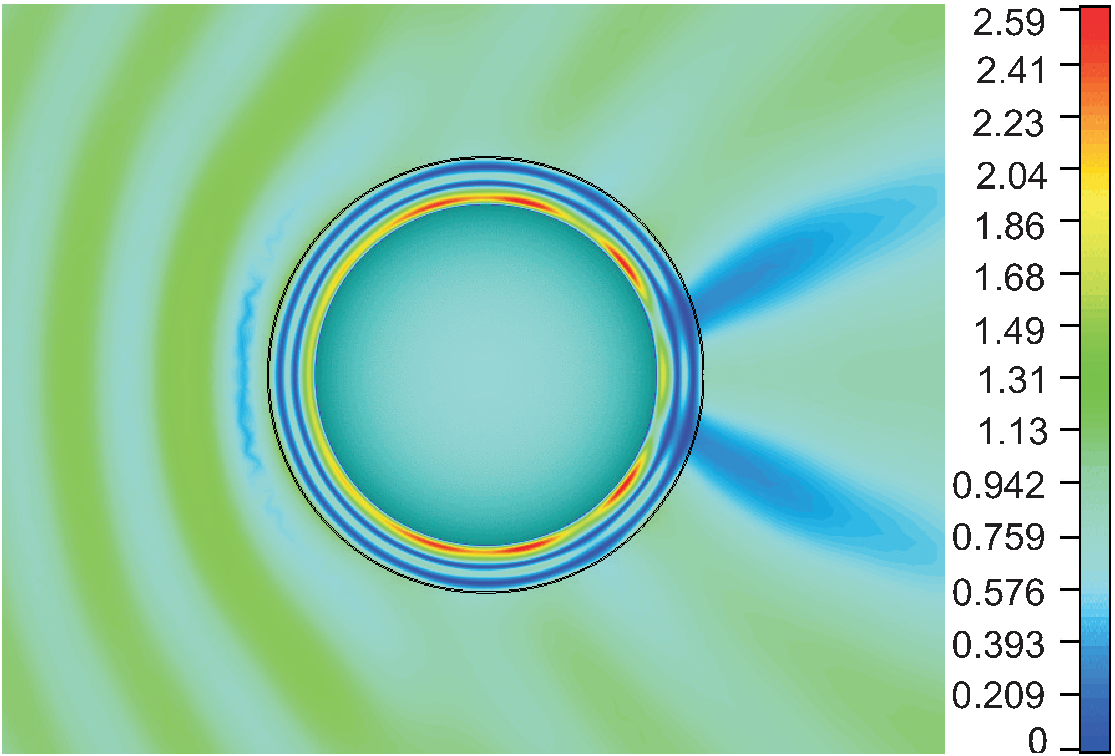
\includegraphics[width=0.7\linewidth]{W08-planeYZ-E-abs}}
  \end{minipage}\\
  \vfill
  \begin{minipage}[ht]{0.99\linewidth}
    \centering{а)}
  \end{minipage}\\
  \vfill
  \begin{minipage}[ht]{0.95\linewidth}
    \centering{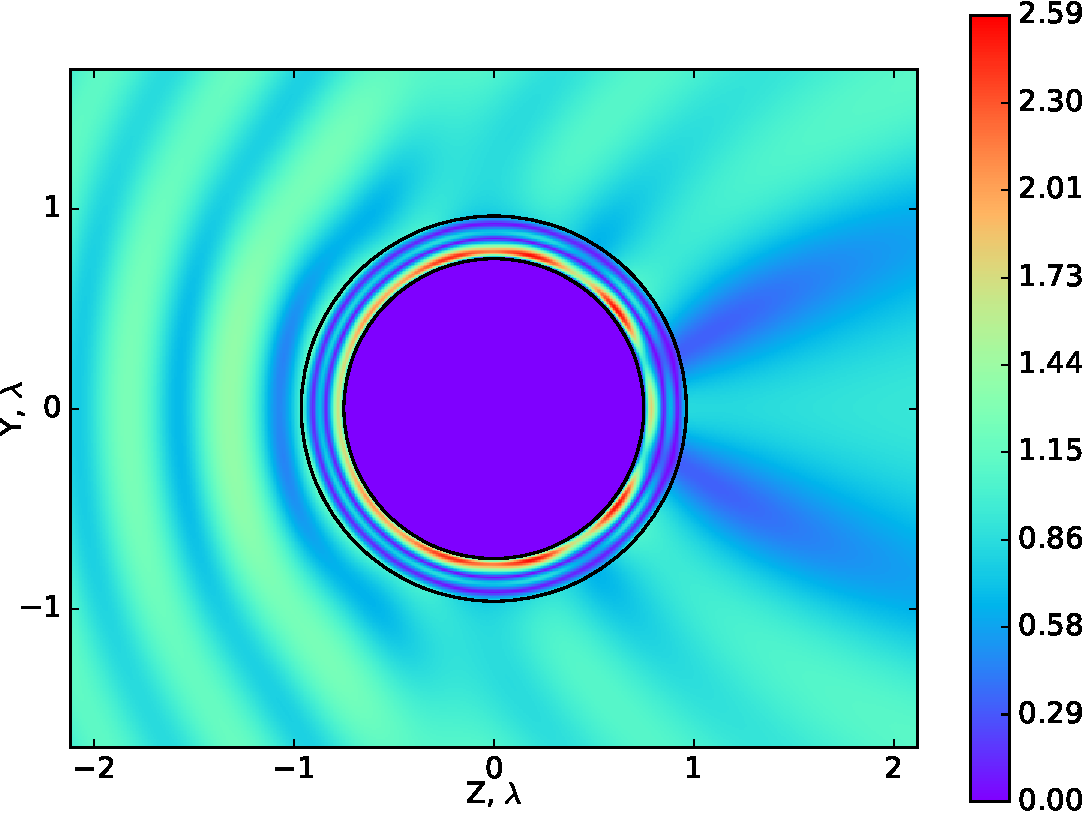
\includegraphics[width=0.79\linewidth]{PEC-index-dv-R4-YZ-Eabs}}
  \end{minipage}\\
  \vfill
  \begin{minipage}[ht]{0.99\linewidth}
    \centering{б)}
  \end{minipage}
  \caption{32-слойное диэлектрическое маскирующее покрытие вокруг
    сферы из идеального электрического проводника. (a) результат
    моделирования в CST MWS с помощью FEM в частотной области, (б)
    результат расчёта ближнего поля по выражениям из
    раздела~\ref{sec:Mie}. Цвет характеризует величину электрического
    поля $|E|/|E_0|$. Волна падает слева направо.\label{img:e32layer}}
\end{figure}

Моделирование с помощью CST~\cite{CST-web} производилось в частотном
пространстве с использованием метода конечных элементов. Дискретизация
модели проводилась нерегулярной тетрагональной сеткой, общее число
элементов разбиения составило около 4 миллионов.  С целью уменьшения
объёма моделирования использовались плоскости симметрии, имеющиеся в
модели. Было выбрано открытое граничное условие с заданным уровнем
отражения -40~dB. Моделирование при этом продолжалось приблизительно
сутки, что существенно отличается от случая с использованием теории
Ми, где для той же системы расчёт занял около 5 минут.

В данном случае совпадение результатов моделирования оказалось очень
хорошим, различие между двумя методами расчёта составило менее 0.4\%
для величины полного сечения рассеяния. Картины ближнего поля
оказались очень похожи, как по форме распределения, так и по 
величине (некая проблема отображения заключается в том, что для
расчёта по теории Ми не удалось подобрать ту же цветовую гамму для
шкалы значений электрического поля).

\section{Выводы}

В главе рассмотрены различные методы теоретического исследования
взаимодействия электромагнитного поля и многослойной сферической
наночастицы. Лучше всего для этого подходит теория Ми, для расчёта был
выбран алгоритм с максимальной численной устойчивостью.  Были получены
явные рекуррентные соотношения для коэффициентов Ми в расчёте
локальных полей, выраженные через логарифмические производные функций
Риккати-Бесселя.  Эти соотношения были добавлены в компьютерную
программу, выполняющую вычисления в рамках задачи Ми. Корректность
полученных выражений и работы модифицированной программы была
проверена на ряде примеров с использованием результатов разных
авторов, а также других численных и аналитических методов.



% ссылки на собственные работы:~\cite{vakbib1, confbib1}
% Сошлёмся на приложения: Приложение \ref{AppendixA}, Приложение \ref{AppendixB2}.
% Сошлёмся на формулу: формула \eqref{eq:equation1}.
% Сошлёмся на изображение: рисунок \ref{img:knuth}.

% Используя команду \verb|\labelcref| из пакета \verb|cleveref|, можно
% красиво ссылаться сразу на несколько формул
% (\labelcref{eq:equation1,eq:equation3,eq:equation2}), даже перепутав
% порядок ссылок \verb|(\labelcref{eq:equation1,eq:equation3,eq:equation2})|.
\clearpage           % Глава 1
\chapter{Метод стохастической оптимизации при решении обратной задачи
  теории Ми} \label{chapt2}

\section{Сравнение методов стохастической оптимизации}
\label{sec:construct-review}

Прогресс в области нанофотоники, как и во многих других разделах
физики, происходит при одновременном развитии теории и эксперимента,
которые оказываются тесно связаны между собой.  Эксперимент определяет
меру правильности теоретических построений и, в то же время, является
источником новых физических эффектов. В последнем случае, определяющей
становится роль теоретического анализа, необходимого для выделения
сути явления из вороха возможных побочных факторов.  Аналогично, при
исследовании оптических свойств наночастиц можно брать результаты
эксперимента и потом проверять, насколько они соотносятся с
существующими моделями. Либо можно вначале находить теоретически
дизайны с новыми физическими свойствами, а уже потом проверять их
экспериментально.  Учитывая высокую стоимость и трудоёмкость
эксперимента в области оптики наночастиц вариант с предварительным
теоретическим анализом проблемы оказывается более рациональным.

Теория Ми позволяет изучать целый ряд физических величин, в число
которых входят, например, сечения рассеяния и поглощения,
распределение электромагнитного поля как внутри, так и вблизи
наночастицы.  Дополнительно в теории Ми есть возможность разделять
вклады связанные с дипольными резонансами, квадрупольными и
мультиполями большего порядка. Такое разнообразие сильно затрудняет
решение обратной задачи, где требуется определить дизайн наночастицы
для достижения заданных характеристик взаимодействия с падающей
волной. Кроме того, заданным параметрам может соответствовать
несколько дизайнов или ни одного.

Попытка решать эту задачу полностью аналитически сразу приводит к
необходимости выбора тех характеристик взаимодействия поля с частицей,
чьи значения будут определять наиболее подходящий дизайн. Другими
словами, необходимо будет решать обратную задачу отдельно для сечения
рассеяния, отдельно для коэффициента усиления поля и так далее, а это
многократно увеличивает объём необходимых работ. Более того,
использование только аналитического подхода заведомо оказывается
неприменимым при учёте экспериментально измеренных дисперсионных
зависимостей материальных параметров. Например, когда требуется
определить дизайн частицы из заданных металлов для получения нужных
рабочих характеристик в какой-то полосе частот и дополнительно
найти оптимальную длину волны внутри выбранного диапазона.  В
результате, наиболее универсальным представляется численное решение,
когда компьютерная программа выбирает параметры дизайна наночастицы
максимально приближенные к оптимальным.

Для численного решения обратную задачу теории Ми можно
переформулировать в общем виде. Будем рассматривать расчёт по теории
Ми в виде некой сложной функции, которая в контексте численного
решения называется целевой функцией $f(\mathbf{x})$, в англоязычной
литературе используются термины objective function или fitness
function.  Целевая функция получает вектор значений для входных
параметров, который в нашем случае является списком из показателей
преломления и толщин каждого слоя. Результат вычисления целевой
функции получается в виде скаляра, который при решении задачи Ми может
быть как значением физической величины, получаемой из расчёта, так и
некой искусственной композицией, характеризующей отклик системы в
целом, например, отношение сечений рассеяния и поглощения. Тогда
обратную задачу можно сформулировать, как поиск такого вектора входных
параметров для целевой функции, который позволял бы получить на выходе
значение, равное заранее заданной величине или наиболее приближенное к
ней. Таким образом, на этапе формулирования общего вида задачи
снимается вопрос о существовании её решения: если нет точного ответа,
то будет получено приблизительное значение. Этого может оказаться
достаточно для обеспечения потребностей широкого круга практических
задач.

При такой постановке вопроса становится возможным использовать
различные методы численной оптимизации, которые позволяют находить
положение экстремума у произвольной функции. Поиск вектора входных
параметров $\mathbf{x_t}$, который позволяет получить целевое значение
$y_t=f(\mathbf{x_t})$, сводится к поиску минимума для новой целевой
функции $\left|f(\mathbf{x})-y_t\right|$.

При выборе конкретного метода оптимизации возникает сложность,
обусловленная их огромным количеством и большим числом
модификаций каждого из них. При выборе метода применительно к задаче
Ми были использованы следующие предпосылки:
\begin{itemize}
\item \label{ref:why-jade} Несмотря на то, что решение Ми является аналитическим и
  выражается разложением в ряд по сферическим векторным
  гармоникам, одновременное нахождение производных для зависимости от
  радиуса и материального параметра оказывается громоздким даже в
  случае однородной сферы. Это тем более верно для случая
  произвольного числа сферических слоёв, где решение получается в виде
  рекуррентного соотношения.  Таким образом, метод оптимизации не
  должен требовать для своей работы нахождения значений производных
  оптимизируемой функции, что особенно актуально в случае, когда
  одновременно оптимизируются и толщина, и показатель преломления
  каждого слоя.
\item Решение образовано осциллирующими функциями и, как следствие,
  будет содержать большое количество локальных экстремумов. Поэтому
  алгоритмы оптимизации, требующие особого отношения к подобным
  случаям, оказываются заведомо менее производительными.
\item Параметры оптимизации и оптимизируемая величина являются
  вещественными числами.
\end{itemize}

Всё вместе это приводит к необходимости исключить из рассмотрения
такие популярные алгоритмы, как метод наискорейшего спуска (требующий
вычисления градиента), симплекс--метод Нелдера--Мида (есть сложность с
локальными экстремумами) и аналогичные им. В результате, приходится
ограничить выбор стохастическими подходами, среди которых наиболее
распространёнными являются генетические
алгоритмы~\cite{Goldberg-GA-1989}, методы  роя
частиц~\cite{Kennedy-PSO-1995} и дифференциальной
эволюции~\cite{Storn-DE-first-1997}.  Все эти алгоритмы используют
метод <<проб и ошибок>>.  Несколько пробных решений, называемых
индивидами, генерируются случайным образом и многократно (итеративно)
улучшаются в надежде найти некое удовлетворительное решение. Качество
решения оценивается целевой функцией, которая должна быть
сформулирована в оптимизируемой задаче.  Полная группа индивидов
образует популяцию.  Состояние популяции на конкретном шаге итерации
называется поколением.  Переход между поколениями осуществляется в
соответствии с рядом относительно простых правил, которые составляют
сущность определённого алгоритма.

Генетические алгоритмы обычно рассматривают вещественные числа в виде
набора битов.  В отличие от них, методы роя частиц и дифференциальной
эволюции могут работать в непрерывном пространстве вещественных
входных параметров естественным образом (используя возможность
сложения и вычитания векторов пробных решений), что делает их гораздо
более удобными для физических и инженерных задач.  Производительность
этих алгоритмов зависит от правильного выбора значений некоторых
внутренних параметров.  Использование адаптивных версий алгоритмов
упрощает задачу оптимизации: для них значения внутренних параметров
настраиваются автоматически при переходе между поколениями. Как
правило, адаптивным алгоритмам нужно гораздо меньше (более чем на
порядок) итераций, чем неадаптивным, чтобы добиться того же результата
оптимизации. Такое поведение тесно связано с так называемой теоремой
<<об отсутствии бесплатных обедов>>~\cite{Wolpert-NFL-1997} (No free
lunch theorem). Она была доказана в достаточно общем виде и,
упрощённо, утверждает, что если в наборе методов оптимизации какой-то
один метод оказался лучше для выбранного множества целевых функций, то
обязательно существует другое множество целевых функций, где этот
метод перестанет быть лучшим. В адаптивном случае выбор наилучшего
алгоритма происходит прямо во время оптимизации для текущей фазы
поиска минимума у конкретной тестовой функции, что и обуславливает
значительное необходимого числа итераций. Хотя, разумеется, можно
сконструировать такие тестовые функции, которые не будут требовать
адаптации алгоритма, и для них адаптивные методы могут несколько
проиграть неадаптивным (вследствие наличия дополнительных вычислений,
необходимых для адаптации).

Сравнение~\cite{Gong-compare-EA-2014,Kang-compare-EA-RABC-2011}
адаптивного алгоритма дифференциальной эволюции
JADE~\cite{Jingqiao-JADE-2009} с адаптивной оптимизацией методом роя
частиц~\cite{Zhan-APSO-2008} и многими другими методами показало
превосходство JADE или результат сопоставимый с лучшими из числа
протестированных методов оптимизации для большинства стандартных
тестов~\cite{Schwefel-1981,Rosenbrock-1960,Muhlenbein-1991,back-1996,Griewank-1981}.
Такое преимущество и относительная простота JADE послужили
основанием для того, чтобы выбрать его в качестве основного алгоритма 
оптимизации в настоящей работе. Дополнительно для JADE была
реализована улучшенная скорость скрещивания (по алгоритму
PMCRADE~\cite{Li-PMCRADE-2011}), получившийся метод оптимизации будет
применён в последующих главах диссертации.



\section{Реализация алгоритма JADE в виде программы}
\label{sec:jade}

Часть технических моментов, касающихся выбора языка программирования и
вопросов производительности итоговой программы, была изложена в
разделе~\ref{sec:code} и остаётся верной для реализации алгоритма
стохастической оптимизации. Тем не менее, есть ряд отличий и
дополнительных факторов.

Прежде всего это связано с тем, что на момент начала работ не было
обнаружено готового к применению программного кода алгоритма JADE, поэтому его
реализация полностью выполнена автором настоящей диссертации. Это
позволило, во-первых, выбрать наиболее подходящий для реализации язык
программирования и, во-вторых, избежать возможных сложностей с
лицензированием чужого исходного кода. В частности, тип лицензии для
разработанной библиотеки оптимизации был выбран полностью
совместимым с лицензией использования программы для расчётов по
теории Ми.

Важным является вопрос об использовании генераторов псевдослучайных
чисел (ГПСЧ). Для работы стохастического оптимизатора требуется
хороший источник энтропии, однако, в стандартной библиотеке языка
Си\texttt{++} долгое время этому вопросу не уделялось должное
внимание. В стандарте языка Си\texttt{++}11, принятом в 2011 году, была
добавлена новая библиотека \verb+random+, реализующая целый ряд
ГПСЧ. Прежде всего, это Ranlux~\cite{Luscher-RNG-Ranlux-1994}, который
входит в число основных ГПСЧ для моделирования методом Монте--Карло, и
MT19937~\cite{Matsumoto-RNG-MT-1998}, использующий вихрь Мерсенна. В
последние годы MT19937 завоевал значительную популярность благодаря
своей высокой производительности и большому периоду при достаточно
хороших статистических показателях. Поэтому MT19937 является ГПСЧ
используемым по умолчанию в самых разнообразных программах, включая
широко известную Matlab Mathworks~\cite{Matlab-web}. Таким образом, для разработки
стохастического оптимизатора подходят только относительно недавние
стандарты языка, начиная с версии Си\texttt{++}11 и более поздние.

Использование относительно свежей спецификации стандарта для языка
программирования Си\texttt{++} обладает дополнительными
преимуществами. Из возможностей, появившихся в Си\texttt{++}11,
активно использовался новый синтаксис работы с перечисляемыми
коллекциями, механизм автоматического определения типа переменной на
этапе компиляции и 
задание значений по умолчанию для данных класса в
заголовочном файле. Всё вместе это заметным образом сокращает время,
необходимое для разработки новой функциональности и её дальнейшей отладки.

Современные процессоры, используемые для проведения расчётов, обычно
 содержат несколько вычислительных ядер, что позволяет
одновременно выполнять такое же количество потоков вычислений. Так как расчёты
значений целевой функции каждого индивида в рамках одного
поколения стохастической оптимизации не зависят друг от друга, то они
хорошо подходят для параллельного выполнения. Другая возможность в
полной мере задействовать вычислительные способности современных
процессоров связана со случайной природой выполняемой
оптимизации. Итоговый результат оптимизации при одних и тех же
исходных параметрах может различаться, что лучше всего заметно в
случае, когда есть несколько похожих по форме и значению локальных
минимумов, а глобальный минимум отсутствует. В этом случае финальное
значение, полученное при оптимизации, с приблизительно равной
вероятностью может оказаться в каждом из таких минимумов. Чтобы
определить возникновение подобной ситуации необходимо несколько
независимых запусков оптимизатора, каждый из которых может выполняться
на своём вычислительном ядре.

В настоящей работе для реализации был выбран последний вариант. Такой
выбор обоснован его относительной простотой и тем, что типичное
количество необходимых запусков оптимизатора при решении
задачи Ми приблизительно совпадает с числом вычислительных ядер у
современных процессоров в стационарных компьютерах (около
десяти). Впрочем, предусмотрена возможность реализации первого
варианта параллельного выполнения (когда в рамках одной оптимизации
вычислительные ядра используются для одновременного расчёта
нескольких значений целевой функции). Этот вариант станет предпочтительным
при использовании оптимизатора на суперкомпьютерном кластере, где число
вычислительных ядер заметно превышает количество необходимых запусков
оптимизации, но ещё меньше или сравнимо с числом индивидов в поколении.

Также существует возможность гибридного похода. В случае, когда
количество вычислительных ядер оказывается больше числа индивидов в
поколении, то их использование для одного запуска оптимизации
становится неэффективным из-за структуры информационных зависимостей в
алгоритме дифференциальной эволюции. Дело в том, что расчёт значений
целевой функции для очередного поколения оптимизации можно начинать
только после того, как будет завершён расчёт этих значений для
текущего поколения, так как на их основе проводится отбор лучших индивидов
для генерации нового поколения. Поэтому,
например, в случае, когда число вычислительных ядер в два раза
превышает количество индивидов в поколении, то наиболее рациональным
является запуск двух независимых оптимизаций.

Выбранный алгоритм допускает и более сложные схемы балансировки,
которые могут быть реализованы в случае необходимости. Например, если
число ядер не кратно количеству индивидов в поколении, то одним из
возможных вариантов является использование общей очереди
вычислений. Каждый из независимых запусков оптимизации размещает в ней
аргументы своих индивидов текущего поколения для расчёта целевой
функции.  Вычислительные ядра разбирают эту очередь, выполняют расчёт
и возвращают результат соответствующему процессу оптимизации. Такой
метод балансировки должен обеспечить высокую эффективность в случае,
когда число индивидов в текущем поколении в сумме по всем запускам
оптимизации заметно превышает количество вычислительных ядер.

Указанная выше особенность структуры информационных зависимостей в
алгоритме дифференциальной эволюции приводит к существованию верхнего
предела его эффективной параллелизации.  А именно, эффективно может
быть использовано число вычислительных ядер равное общему количеству
индивидов в текущем поколении всех запусков оптимизации. При
дальнейшем увеличении числа ядер величина параллельной эффективности
будет падать.

Однако, стоит учитывать, что, как правило, применение
суперкомпьютерных кластеров становится оправданным в случае
необходимости решения вычислительно трудоёмких задач, когда разовое
вычисление целевой функции само по себе требует заметного
времени. Поэтому в качестве независимого вычислителя, выполняющего
расчёт значения целевой функции, алгоритм оптимизации может вместо
одного ядра  рассматривать процессор целиком, вычислительный
узел или их группу. Общая параллельная эффективность при этом
будет определяться не только эффективностью оптимизатора, но и тем,
насколько эффективно может быть выполнено распараллеливание расчёта
целевой функции.  В качестве примера таких целевых функций можно
привести полноволновые расчёты трёхмерных моделей, использующих метод
конечных элементов.

Для реализации алгоритма, обеспечивающего параллельное выполнение
оптимизации, были выбраны программные библиотеки, поддерживающие
стандарт Message Parsing Interface (MPI). Это позволяет запускать
оптимизацию в несколько потоков как на одиночных процессорах, так и на
суперкомпьютерных кластерах. Несмотря на то, что на момент написания
диссертации поддерживался только самый простой вариант параллелизации
(количество используемых вычислительных ядер определяет число
независимых запусков оптимизатора, выполняемых одновременно) подобная
совместимость с суперкомпьютерными кластерами оказалась удобной: на
одном кластере можно запускать несколько разных задач оптимизации. 
Для этого через менеджер ресурсов и
задач кластера запрашивается необходимое число вычислительных ядер.

С помощью штатных возможностей функций MPI был реализован сбор
результатов оптимизации по всем независимым запускам, после чего
выполнялся расчёт статистических параметров: среднего значения и
среднеквадратичного отклонения. Это позволило удобным образом
организовать тестирование оптимизатора на ряде стандартных функций,
где для каждой по общепринятой методике проводится 50 запусков.
 Более подробно вопрос тестирования оптимизатора
будет рассмотрен в разделе~\ref{sec:test-jade}.

В теории разработки программного обеспечения широко известны несколько
техник, которые позволяют создавать, отлаживать, развивать и
поддерживать сложные продукты.  Их использование позволяет
значительно снизить стоимость работы программиста, или, другими
словами, существенно упростить процесс разработки.  Недостатком ряда
подобных техник является наличие дополнительных накладных расходов на
их выполнение.  В случае, если создаваемая программа оказывается
недостаточно большой и сложной, то их использование может не окупиться
в краткосрочной перспективе.  Часть техник оказываются специфичны для
каких-то языков программирования или выбранной парадигмы
(функциональной, императивной, объектно-ориентированной и~т.д.),
однако, существует несколько общих принципов, применение которых не
требует больших затрат времени. В их число входят техника сокрытия
сложности за счёт разделения абстракций и защитное программирование,
которые были использованы при разработке оптимизатора в настоящей
главе.

Защитное программирование предполагает, что каждая вызываемая функция
или подпрограммы должна сама проверять корректность и
самосогласованность используемых данных. Это заметно упрощает
разработку, так как в этом случае проверка данных и их обработка
оказываются локализованы в теле одной подпрограммы. Если на
каком-то этапе данные перестали соответствовать ожиданиям
разработчика, то такая подпрограмма сразу даст об этом знать. В
противном случае, о наличии сбоя можно будет судить только по
итоговому результату работы программы, поиск места в программе,
которое привело к ошибке, займёт значительно больше времени. После
окончания отладки программы и верификации её работы на ряде тестовых
примеров есть возможность отключить такие проверки, таким образом, их
наличие не скажется на итоговой производительности программы.

Сокрытие сложности во многом основано на более общем принципе,
согласно ему выполнение сложной задачи (которая не может быть
выполнена сразу и целиком) разбивается на несколько подзадач. В
терминах языка программирования Си\texttt{++} подзадачи называются
методами класса и функциями.  В общем случае при программировании
регламентируется количество подзадач, и возникает требование
минимальной связности между ними.  Ограничение на число подзадач
определяется особенностями человеческого восприятия. Если их 
становится более 10--15 штук, то для них резко возрастает сложность анализа 
взаимного влияния.  Эмпирически это ограничение широко известно как
<<правило одного экрана>>.  Так как при разработке декомпозиция
выражается в виде описания функции или метода класса, то не
рекомендуется делать такое разбиение, которое занимает более 25 строк
в тексте программы (это высота экрана стандартного
терминала).  С учётом строк, которые тратятся на формальное определение
функции, форматирование, логические конструкции, комментарии и тому
подобное, то в результате получается не более 10--15 логически
самостоятельных подзадач. На это число автор диссертации и
ориентировался при реализации алгоритма стохастической оптимизации.


Более важным при сокрытии сложности программы является требование
минимальной связности подзадач, что формально может быть
измерено числом передаваемых между ними логически обособленных единиц информации.
Если, например, основная задача программы
состоит в создании, модификации и дальнейшей пересылки какой-то одной
структуры данных, то только эти три подзадачи и надо включать в
декомпозицию на первом уровне разбиения из-за их слабой связности. Если
подзадача оказалась сама по себе достаточно сложной, то она
подвергается дальнейшей декомпозиции, что приводит к возникновению
иерархии подпрограмм.  Число в 10--15 подзадач, указанные ранее, это
верхний предел, достижение которого сигнализирует, что какая-то
группа подзадач скорее всего может быть выделена в отдельную подзадачу,
так как является более связанной. Например, формально это можно
понять, если такая группа подзадач использует какие-то данные, которые
не используются несколькими подзадачами до и после неё.

При реализации уже существующего алгоритма дифференциальной эволюции
разбиение на подзадачи происходит естественным образом. Сам по себе
алгоритм в тексте программы был оформлен в виде отдельной логической
единицы, объединяющей  данные и методы, необходимые
для проведения оптимизации (в Си\texttt{++} такое
объединение называется классом). Среди методов класса, реализующих
ключевые шаги алгоритма оптимизации, можно отметить селекцию, мутацию,
кроссовер, адаптацию. В них используется ряд вспомогательных методов,
которые отвечают за создание нужных случайных распределений, выборку
индивидов для генерации следующего поколения и так далее. Ряд
интерфейсных методов, которые доступны для использования внешними
программами, отвечает за настройку параметров,
инициализацию внутренних структур данных и запуск оптимизации.

Указанные рекомендации часто используются программистами на уровне,
близком к интуитивному, и могут трактоваться довольно творчески.  Это
связано с тем, что всегда существуют ограничения по времени, которое
может быть потрачено на разработку. Поэтому в небольших проектах,
связанных с исследовательской деятельностью, более рациональным может
оказаться быстрое получение результата при достаточно плохой структуре
программы. Так как она в дальнейшем не используется, то существенное
увеличение расходов на поддержание и развитие такого кода
отсутствует. В случае реализации алгоритма стохастической оптимизации
возможная область применения такой программы довольно широка. Поэтому
вопросу структурирования разрабатываемой библиотеки оптимизации было
уделено достаточно много времени.  Опыт регулярного использования
результата этой работы автором диссертации на протяжении почти 3-х лет подтвердил
правильность выбранного подхода.  В частности, когда потребовалось
добавить новую функциональность, а именно, возможность задавать
начальное значение для части индивидов в популяции, это удалось
сделать без существенных затрат сил и времени, сохранив обратную
совместимость с программами, использовавшими предыдущую версию
оптимизатора.

На этапе проектирования программы оптимизатора был допущен ряд ошибок,
большую часть которых удалось исправить при отладке и
тестировании. Оставшиеся не влияют на корректность получаемых
результатов, но несколько затрудняет использование оптимизатора.
Наиболее существенной среди них является выбор в пользу <<кодов
ошибок>> для отработки программой внештатных ситуаций вместо
использования <<механизма исключений>>.  Такое решение было принято в
целях экономии времени, так как начальное изучение методик применения
механизма исключений в Cи\texttt{++} потребовало неожиданно много
усилий, а коды ошибок являются хорошо проверенной и часто используемой
техникой при создании программ на родственном языке Си. Поэтому, среди
собственных переменных класса была объявлена специальная переменная
\verb+error_status_+, каждый метод записывает туда
значение кода ошибки, соответствующее какому-то типу случившейся
внештатной ситуации.  В подавляющем большинстве случаев дальнейшее
выполнение программы можно прекратить, сообщив пользователю о типе
возникшей ошибке и месте её возникновения, что и было
реализовано. Недостатком этого подхода является дублирование кода в
теле различных методов класса для обработки аналогичных внештатных
ситуаций, что увеличивает общий объём кода, и, как следствие,
затрудняет его дальнейшее усовершенствование.

Кроме того, применение кодов ошибок не позволяет в полной мере
разрешить ситуацию, когда проблема возникает в подпрограмме,
вычисляющей значение оптимизируемой функции. Дело в том, что эта
функция задаётся полностью независимо, поэтому у неё нет доступа к
собственным переменным класса оптимизатора и она может, например,
использовать любые свои коды ошибок. Так как библиотека оптимизатора
должна быть универсальной, то возможно два варианта решения такой
коллизии. Во-первых, в документации можно объявить коды ошибок,
которые может возвращать оптимизируемая функция. Это ограничение не
всегда может быть выполнено в случае, когда такая функция является
уже готовой к использованию достаточно сложной
программой. Дополнительно, возникнет новая связь, существование
которой обусловлено техническими моментами и, как следствие нарушает
требование минимальной логической связности между частями программы:
явная передача кода ошибки никак не обоснована в рамках задачи
оптимизации.  Во-вторых, можно отказаться от кодов ошибок и
использовать механизм исключений, который существует на уровне языка
синтаксиса Си\texttt{++}.  В случае, если оптимизируемая функция уже
использует исключения для своей работы, такой подход представляется
наиболее естественным.  Возникновение неявной связи (создаваемое
исключение передаётся на более высокий уровень иерархии подпрограмм)
частично компенсируется её однонаправленным характером и
возможностью убрать явную обработку исключений на промежуточных уровнях
иерархии.  Однако подобная возможность одновременно является и
основным недостатком механизма исключений, так как генерация
исключения и его обработка могут оказаться разнесены по самым
неожиданным частям программы.  Это может привести к существенным
затруднениям для программиста в случае необходимости разобраться, что
происходит во внештатной ситуации, поэтому при применении механизма
исключений в Си\texttt{++} необходимо вдумчиво выбирать места их
обработки в тексте программы.

В полной мере необходимость использования механизма исключений стала
понятна при практическом применении оптимизатора для создания дизайнов
наночастицы.  Дело в том, что в некоторых редких случаях входные
параметры, получаемые с помощью оптимизатора, приводили к
неустойчивому расчёту по теории Ми. Сообщение о факте возникновения
неустойчивости передавалось по механизму исключений. Так как класс
оптимизатора уже был готов и использовал коды ошибок, то было принято
компромиссное решение. В результате используются
оба подхода для разрешения внештатных ситуаций. В случае
необходимости дальнейшего улучшения оптимизатора запланированы работы
по миграции на использование только механизма исключений. Это позволит
увеличить степень унификации кода и упростит его разработку и
поддержание.

\section{Тестирование реализации алгоритма JADE}
\label{sec:test-jade}
Применение численных методов оптимизации никогда не может
гарантировать, что получится найти глобальный экстремум, а в случае
произвольной функции нет гарантий, что он будет  хотя бы
локальным экстремумом.  В предельном случае, рассмотрим ступенчатую
функцию с минимумом в выколотой точкой.  Очевидно, что вероятность
попасть в эту точку крайне мала.  Более того, если, например,
координата этой точки задана иррациональным числом, то из-за
дискретного характера представления чисел, используемого компьютером, получить в
точности это значение на выходе из оптимизатора не является возможным
даже теоретически.  Впрочем, поиск минимума подобной функции может
быть затруднительным и при использовании исключительно аналитических
методов.  Стоит отметить, что при решении физических задач подобные
функции попадаются достаточно редко.  Учитывая предпосылки,
перечисленные на странице~\pageref{ref:why-jade}, применение
стохастической оптимизации в настоящей работе является вполне
обоснованным.

Другой крайностью являются функции, у которых нет единого глобального
экстремума и/или есть большое число локальных экстремумов.  Ранее уже
обсуждался случай, когда есть несколько похожих по форме и значению
локальных минимумов, тогда стохастический оптимизатор будет находить
их с приблизительно равной вероятностью.  В случае, если локальные
минимумы сильно отличаются друг от друга, то предсказание становится
затруднительным.  Например, пусть есть два локальных минимума в общем
ровном фоне, первый --- узкий, а второй --- широкий (сравнивается ширина
на полувысоте). При прочих равных, стохастическому оптимизатору проще
найти широкий минимум. В случае если верхняя часть у первого
локального минимума во много раз больше, чем ширина второго, а у
него, в свою очередь, подобного расширения нет (например его стенки
являются практически вертикальными), то ситуация становится
неоднозначной.  С одной стороны, оптимизатору по-прежнему проще
попасть во второй минимум при случайной мутации индивидов. В то же
время, вероятность попасть в верхнюю часть первого минимума ещё
выше. Так как значение целевой функции в этой области находятся ниже
среднего фона, то в ней будут скапливаться индивиды, вырастет число
попыток найти в её окрестности глобальный минимум.  В итоге,
значительно вырастет вероятность нахождения узкого минимума.  Подобная
неоднозначность в результате работы оптимизатора и приводит к
необходимости его многократного запуска, что было подробно рассмотрена
в разделе~\ref{sec:jade}.

Ещё одним семейством функций, у которых нахождение экстремума может
оказаться достаточно сложной задачей для локальных методов
оптимизации, характеризуются особенностью в виде долины (при поиске
минимума). В этом случае можно выделить линию <<низа>> долины, при
движении вдоль которой плавно проходится значение минимума, а
в направлении поперёк неё функция резко возрастает на <<склонах>>
долины. Подобный протяжённый характер минимума вводит в заблуждение
большинство алгоритмов оптимизации: они достаточно быстро попадают в
низ долины, однако плохо справляются с движением по нему, если он
обладает заметной кривизной. Это оказывается верным для
большинства итеративных методов, в том числе и метода градиентного
спуска. Он в такой ситуации демонстрирует движение мелким
зигзагом. Типичным представителем этого семейства функций является
функция Розенброка~\cite{Rosenbrock-1960}
(см. $f_5$ в таблице~\ref{tbl:test-functions}).
% TODO check longtable positions before final release.
%%%%%%%%%%%%%%%%%%%%%%%%%%%%%%%%%%%%%%%%%%%%%%%%%%%%%%%%%%%%%%%%%%%%%%%%% 
%%%%%%%%%%%%%%%%%%%%%%%%%%%%%%%%%%%%%%%%%%%%%%%%%%%%%%%%%%%%%%%%%%%%%%%%%
%%%      Table Funсtions     %%%%%%%%%%%%%%%%%%%%%%%%%%%%%%%%%%%%%%%%%%%%
%%%%%%%%%%%%%%%%%%%%%%%%%%%%%%%%%%%%%%%%%%%%%%%%%%%%%%%%%%%%%%%%%%%%%%%%% 
%%%%%%%%%%%%%%%%%%%%%%%%%%%%%%%%%%%%%%%%%%%%%%%%%%%%%%%%%%%%%%%%%%%%%%%%%
\begingroup % Ограничиваем область видимости arraystretch
\needspace{2\baselineskip}
\renewcommand{\arraystretch}{1.6}%% Увеличение расстояния между рядами, для улучшения восприятия.
\begin{longtabu} to \textwidth {@{}>{\setlength{\baselineskip}{0.7\baselineskip}}X[1.1mc]>{\setlength{\baselineskip}{0.7\baselineskip}}X[mc]X[4]@{}}
        \caption{Тестовые функции для оптимизации, $D$ ---
          размерность. Для всех функций значение в точке глобального
          минимума равно нулю.\label{tbl:test-functions}}\\% label всегда желательно идти после caption 
        
        \toprule     %%% верхняя линейка
        Имя           &Стартовый диапазон параметров &Функция  \\ 
        \midrule %%% тонкий разделитель. Отделяет названия столбцов. Обязателен по ГОСТ 2.105 пункт 4.4.5 
        \endfirsthead

        \multicolumn{3}{c}{\small\slshape (продолжение)}        \\ 
        \toprule     %%% верхняя линейка
        Имя           &Стартовый диапазон параметров &Функция  \\ 
        \midrule %%% тонкий разделитель. Отделяет названия столбцов. Обязателен по ГОСТ 2.105 пункт 4.4.5 
        \endhead
        
        \multicolumn{3}{c}{\small\slshape (окончание)}        \\ 
        \toprule     %%% верхняя линейка
        Имя           &Стартовый диапазон параметров &Функция  \\ 
        \midrule %%% тонкий разделитель. Отделяет названия столбцов. Обязателен по ГОСТ 2.105 пункт 4.4.5 
        \endlasthead

        \bottomrule %%% нижняя линейка
        \multicolumn{3}{r}{\small\slshape продолжение следует}  \\ 
        \endfoot   
        \endlastfoot

        сфера         &$\left[-100,\,100\right]^D$   &
        $\begin{aligned}\textstyle f_1(\mathbf{x})=\sum_{i=1}^Dx_i^2\end{aligned}$                                                        \\
        Schwefel 2.22 &$\left[-10,\,10\right]^D$     &
        $\begin{aligned}\textstyle f_2(\mathbf{x})=\sum_{i=1}^D|x_i|+\prod_{i=1}^D|x_i|\end{aligned}$                                     \\
        Schwefel 1.2  &$\left[-100,\,100\right]^D$   &$\begin{aligned}\textstyle f_3(\mathbf{x})=\sum_{i=1}^D\left(\sum_{j=1}^ix_j\right)^2\end{aligned}$                               \\
        Schwefel 2.21 &$\left[-100,\,100\right]^D$   &$\begin{aligned}\textstyle f_4(\mathbf{x})={\rmfamily max}_i\!\left\{\left|x_i\right|\right\}\end{aligned}$                             \\
        Rosenbrock    &$\left[-30,\,30\right]^D$     &$\begin{aligned}\textstyle f_5(\mathbf{x})=\sum_{i=1}^{D-1}\left[100\!\left(x_{i+1}-x_i^2\right)^2+(x_i-1)^2\right]\end{aligned}$ \\
        ступенчатая   &$\left[-100,\,100\right]^D$   &$\begin{aligned}\textstyle f_6(\mathbf{x})=\sum_{i=1}^D\big\lfloor x_i+0.5\big\rfloor^2\end{aligned}$                             \\ 
зашумлённая квартическая  &$\left[-1.28,\,1.28\right]^D$ &$\begin{aligned}\textstyle f_7(\mathbf{x})=\sum_{i=1}^Dix_i^4+rand[0,1)\end{aligned}$\vspace*{2ex}\\
        Schwefel 2.26 &$\left[-500,\,500\right]^D$   &$\begin{aligned}f_8(\mathbf{x})= &\textstyle\sum_{i=1}^D-x_i\,\sin\sqrt{|x_i|}\,+ \\
                    &\vphantom{\sum}+ D\cdot
                    418.98288727243369 \end{aligned}$\\
        Rastrigin     &$\left[-5.12,\,5.12\right]^D$ &
        $\begin{aligned}\textstyle
          f_9(\mathbf{x})=\sum_{i=1}^D\left[x_i^2-10\,\cos(2\pi
            x_i)+10\right]\end{aligned}$\vspace*{2ex}\\
  Ackley        &$\left[-32,\,32\right]^D$     &$\begin{aligned}f_{10}(\mathbf{x})= &\textstyle -20\, {\rmfamily exp}\!\left(-0.2\sqrt{\frac{1}{D}\sum_{i=1}^Dx_i^2} \right)-\\
                    &\textstyle - {\rmfamily exp}\left(\frac{1}{D}\sum_{i=1}^D\cos(2\pi x_i)  \right)  + 20 + e \end{aligned}$ \\
        Griewank      &$\left[-600,\,600\right]^D$
        &$\begin{aligned}f_{11}(\mathbf{x})= &\textstyle \frac{1}{4000}
          \sum_{i=1}^{D}x_i^2 - \prod_{i=1}^D\cos\left(x_i/\sqrt{i}\right) +1     \end{aligned}$ \vspace*{3ex} \\
        штрафная 1    &$\left[-50,\,50\right]^D$     &
        $\begin{aligned}f_{12}(\mathbf{x})= &\textstyle \frac{\pi}{D}
          \Big\{ 10\,\sin^2(\pi y_1) +\\ &+
          \textstyle \sum_{i=1}^{D-1}(y_i-1)^2\left[1+10\,\sin^2(\pi
              y_{i+1})\right] +\\ &+(y_D-1)^2 \Big\} +\textstyle\sum_{i=1}^D u(x_i,\,10,\,100,\,4)            \end{aligned}$ \vspace*{2ex} \\
        штрафная 2    &$\left[-50,\,50\right]^D$     &
        $\begin{aligned}f_{13}(\mathbf{x})= &\textstyle 0.1
          \Big\{\sin^2(3\pi x_1) +\\ &+
          \textstyle \sum_{i=1}^{D-1}(x_i-1)^2\left[1+\sin^2(3 \pi
              x_{i+1})\right] + \\ &+(x_D-1)^2\left[1+\sin^2(2\pi
              x_D)\right] \Big\} +\\ &+\textstyle\sum_{i=1}^D u(x_i,\,5,\,100,\,4)            \end{aligned}$            \vspace*{1ex}\\
        \midrule %%% тонкий разделитель
        \multicolumn{3}{@{}p{\textwidth}}{%
            \vspace*{-4ex}% этим подтягиваем повыше
            \hspace*{2.5em}% абзацный отступ - требование ГОСТ 2.105
            Примечание "---  Для функций $f_{12}$ и $f_{13}$
            используется $y_i = 1 + \frac{1}{4}(x_i+1)$ и
            $u(x_i,\,a,\,k,\,m)=\begin{cases}
k(x_i-a)^m,\quad &x_i >a\\[-0.5em]
0,\quad &-a\leq x_i \leq a\\[-0.5em]
k(-x_i-a)^m,\quad &x_i <-a
\end{cases}$  }   \\        \bottomrule %%% нижняя линейка 
\end{longtabu} \endgroup

Так как заранее предугадать тип функции, который попадётся
оптимизатору при решении произвольной физической задачи не
представляется возможным, то для проверки его работы был использован
стандартный набор
функций~\cite{Schwefel-1981,Rosenbrock-1960,Muhlenbein-1991,back-1996,Griewank-1981}
(см. таблицу~\ref{tbl:test-functions}), часто применяемый другими
авторами в целях тестирования. У каждой функции приводится её имя или
краткое описание, диапазон параметров, внутри которого происходит
поиск минимума, и выражение для вычисления. Всё функции могут
использовать произвольное число независимых переменных, определяемое
размерностью $D$.

Тестирование проводилось в два этапа. На первом сравнивался результат
оптимизатора JADE\texttt{++}, реализованного в рамках настоящей
работы, с оригинальным алгоритмом JADE и другими алгоритмами (были
использованы данные из публикации~\cite{Jingqiao-JADE-2009},
таблицы~\ref{tbl:opt-results-book-30d}
и~\ref{tbl:opt-results-book-100d}). На втором этапе сравнивались
результаты оригинального алгоритма JADE и нескольких его модификаций,
реализованных в настоящей работе
(таблицы~\ref{tbl:opt-results-jade-30d}
и~\ref{tbl:opt-results-jade-100d}).  В этих таблицах приводится
результат оптимизации различными алгоритмами, для удобства восприятия
среднее значение и среднеквадратичное отклонение (указано в скобках)
группируются для каждого сочетания тестовой функции и
алгоритма. Лучший результат для каждой функции дополнительно выделен
шрифтом с полужирным начертанием.

%%%%%%%%%%%%%%%%%%%%%%%%%%%%%%%%%%%%%%%%%%%%%%%%%%%%%%%%%%%%%%%%%%%%%%%%%
%%%%%%%%%%%%%%%%%%%%%%%%%%%%%%%%%%%%%%%%%%%%%%%%%%%%%%%%%%%%%%%%%%%%%%%%%
%%%      Table 30D   %%%%%%%%%%%%%%%%%%%%%%%%%%%%%%%%%%%%%%%%%%%%%%%%%%%%
%%%%%%%%%%%%%%%%%%%%%%%%%%%%%%%%%%%%%%%%%%%%%%%%%%%%%%%%%%%%%%%%%%%%%%%%% 
%%%%%%%%%%%%%%%%%%%%%%%%%%%%%%%%%%%%%%%%%%%%%%%%%%%%%%%%%%%%%%%%%%%%%%%%%
\begingroup % Ограничиваем область видимости arraystretch
%% http://tex.stackexchange.com/questions/278362/apply-italic-formatting-to-every-other-row
%\newcounter{rowcnt}
\newcommand\z{\bfseries}
\renewcommand\altshape{\ifthenelse{\therowcnt = 0 }{%
}{
  \ifnumodd{\value{rowcnt}}{}{\vspace*{-0.8ex}}}
}
\newcolumntype{A}{ >{\altshape}X[1mc]}
\AtBeginEnvironment{tabular}{\setcounter{rowcnt}{1}}
\AtEndEnvironment{tabular}{\setcounter{rowcnt}{0}}

\needspace{2\baselineskip}
\renewcommand{\arraystretch}{0.9}%% Увеличение расстояния между рядами, для улучшения восприятия.
\begin{longtabu} to \textwidth {@{}X[0.3ml]X[0.7mc]AAAA>{\setlength{\baselineskip}{0.7\baselineskip}}AA<{\stepcounter{rowcnt}}@{}}
% \begin{longtabu} to \textwidth {@{}X[0.2ml]X[1mc]X[1mc]X[1mc]X[1mc]X[1mc]>{\setlength{\baselineskip}{0.7\baselineskip}}X[1mc]X[1mc]@{}}
  \caption{Сравнение различных алгоритмов оптимизации. Указанны
    среднее значение и среднеквадратичное отклонение (в скобках) результата
    оптимизации после фиксированного числа итераций (столбец Gen) и для 50 запусков
    каждого алгоритма. Для каждой функции бралось число независимых
    переменных $D=30$.\label{tbl:opt-results-book-30d}}\vspace*{1ex}\\% label всегда желательно идти после caption
  % \vspace*{1ex}     \\
  \toprule %%% верхняя линейка  
\setcounter{rowcnt}{0} &Gen & JADE\texttt{++} & JADE & jDE & SaDE
& DE/rand /1/bin & PSO \\ 
 \midrule %%% тонкий разделитель. Отделяет названия столбцов. Обязателен по ГОСТ 2.105 пункт 4.4.5 
 \endfirsthead
 \multicolumn{8}{c}{\small\slshape (продолжение)} \\ 
 \toprule %%% верхняя линейка
 \setcounter{rowcnt}{0} &Gen & JADE\texttt{++} & JADE & jDE & SaDE
& DE/rand /1/bin & PSO \\ 
 \midrule %%% тонкий разделитель. Отделяет названия столбцов. Обязателен по ГОСТ 2.105 пункт 4.4.5 
 \endhead
 \multicolumn{8}{c}{\small\slshape (окончание)} \\ 
 \toprule %%% верхняя линейка
\setcounter{rowcnt}{0} &Gen & JADE\texttt{++} & JADE & jDE & SaDE
& DE/rand /1/bin & PSO \\ 
 \midrule %%% тонкий разделитель. Отделяет названия столбцов. Обязателен по ГОСТ 2.105 пункт 4.4.5 
 \endlasthead
 \bottomrule %%% нижняя линейка
 \multicolumn{8}{r}{\small\slshape продолжение следует}     \\ 
 \endfoot 
 \endlastfoot
 
$f_{1}$  & 1500 & 3.1E-54  &\z1.3E-54 & 2.5E-28   & 4.5E-20   & 9.8E-14   & 9.6E-42   \\\nopagebreak
    &      & (2.1E-53)& (9.2E-54) & (3.5E-28) & (6.9E-20) & (8.4E-14) & (2.7E-41) \\
$f_{2}$  & 2000 & 6.0E-23  & 3.9E-22   & \z1.5E-23   & 1.9E-14   & 1.6E-09   & 9.3E-21   \\\nopagebreak
    &      & (3.0E-22)& (2.7E-21) & (1.0E-23) & (1.1E-14) & (1.1E-09) & (6.3E-20) \\
$f_{3}$  & 5000 & \z2.7E-92  & 6.0E-87   & 5.2E-14   & 9.0E-37   & 6.6E-11   & 2.5E-19   \\\nopagebreak
    &      & (1.8E-91)& (1.9E-86) & (1.1E-13) & (5.4E-36) & (8.8E-11) & (3.9E-19) \\
$f_{4}$  & 5000 & 8.1E-07  & \z4.3E-66   & 1.4E-15   & 7.4E-11   & 4.2E-01   & 4.4E-14   \\\nopagebreak
    &      & (2.8E-07)& (1.2E-65) & (1.0E-15) & (1.8E-10) & (1.1E+00) & (9.3E-14) \\
$f_{5}$  & 3000 & \z8.0E-02  & 3.2E-01   & 1.3E+01   & 2.1E+01   & 2.1E+00   & 2.5E+01   \\\nopagebreak
    &      & (5.6E-01)& (1.1E+00) & (1.4E+01) & (7.8E+00) & (1.5E+00) & (3.2E+01) \\
$f_{6}$  & 100  & 6.9E+00  & \z5.6E+00   & 1.0E+03   & 9.3E+02   & 4.7E+03   & 4.5E+01   \\\nopagebreak
    &      & (1.8E+00)& (1.6E+00) & (2.2E+02) & (1.8E+02) & (1.1E+03) & (2.4E+01) \\
$f_{7}$  & 3000 & \z6.3E-04  & 6.8E-04   & 3.3E-03   & 4.8E-03   & 4.7E-03   & 2.5E-03   \\\nopagebreak
    &      & (2.3E-04)& (2.5E-04) & (8.5E-04) & (1.2E-03) & (1.2E-03) & (1.4E-03) \\
$f_{8}$  & 1000 & 5.6E-05  & 7.1E+00   & \z7.9E-11   & 4.7E+00   & 5.9E+03   & 2.4E+03   \\\nopagebreak
    &      & (4.0E-05)& (2.8E+01) & (1.3E-10) & (3.3E+01) & (1.1E+03) & (6.7E+02) \\
$f_{9}$  & 1000 & 2.3E-04  & \z1.4E-04   & 1.5E-04   & 1.2E-03   & 1.8E+02   & 5.2E+01   \\\nopagebreak
    &      & (1.2E-04)& (6.5E-05) & (2.0E-04) & (6.5E-04) & (1.3E+01) & (1.6E+01) \\
$f_{10}$ & 500  & 6.4E-09  & \z3.0E-09   & 3.5E-04   & 2.7E-03   & 1.1E-01   & 4.6E-01   \\\nopagebreak
    &      & (9.8E-09)& (2.2E-09) & (1.0E-04) & (5.1E-04) & (3.9E-02) & (6.6E-01) \\
$f_{11}$ & 500  & \z1.1E-07  & 2.0E-04   & 1.9E-05   & 7.8E-04  & 2.0E-01   & 1.3E-02   \\\nopagebreak
    &      & (7.8E-07)& (1.4E-03) & (5.8E-05) & (1.2E-03)  & (1.1E-01) & (1.7E-02) \\
$f_{12}$ & 500  & \z2.6E-16  & 3.8E-16   & 1.6E-07   & 1.9E-05   & 1.2E-02   & 1.9E-01   \\\nopagebreak
    &      & (4.4E-16)& (8.3E-16) & (1.5E-07) & (9.2E-06) & (1.0E-02) & (3.9E-01) \\
$f_{13}$ & 500  & \z1.2E-15  & \z1.2E-15   & 1.5E-06   & 6.1E-05   & 7.5E-02   & 2.9E-03   \\\nopagebreak
    &      & (3.4E-15)& (2.8E-15) & (9.8E-07) & (2.0E-05) & (3.8E-02) & (4.8E-03) \\

    % \vspace*{1ex}     \\
%         \midrule%%% тонкий разделитель
%         \multicolumn{3}{@{}p{\textwidth}}{%
%             % \vspace*{-4ex}% этим подтягиваем повыше
%             % \hspace*{2.5em}% абзацный отступ - требование ГОСТ 2.105
%             Примечание "---  Для функций $f_{12}$ и $f_{13}$
%             используется $y_i = 1 + \frac{1}{4}(x_i+1)$ и
%             $u(x_i,\,a,\,k,\,m)=\begin{cases}
% k(x_i-a)^m,\quad  & x_i >a     \\[-0.5em]
% 0,\quad           & -a\leq x_i \leq a        \\[-0.5em]
% k(-x_i-a)^m,\quad & x_i <-a
% \end{cases}$  }     \\
\bottomrule %%% нижняя линейка 
\end{longtabu} \endgroup


%%%%%%%%%%%%%%%%%%%%%%%%%%%%%%%%%%%%%%%%%%%%%%%%%%%%%%%%%%%%%%%%%%%%%%%%%
%%%%%%%%%%%%%%%%%%%%%%%%%%%%%%%%%%%%%%%%%%%%%%%%%%%%%%%%%%%%%%%%%%%%%%%%%
%%%      Table 100D   %%%%%%%%%%%%%%%%%%%%%%%%%%%%%%%%%%%%%%%%%%%%%%%%%%%%
%%%%%%%%%%%%%%%%%%%%%%%%%%%%%%%%%%%%%%%%%%%%%%%%%%%%%%%%%%%%%%%%%%%%%%%%% 
%%%%%%%%%%%%%%%%%%%%%%%%%%%%%%%%%%%%%%%%%%%%%%%%%%%%%%%%%%%%%%%%%%%%%%%%%
\begingroup % Ограничиваем область видимости arraystretch
%% http://tex.stackexchange.com/questions/278362/apply-italic-formatting-to-every-other-row
% \newcounter{rowcnt}
\newcommand\z{\bfseries}
\renewcommand\altshape{\ifthenelse{\therowcnt = 0 }{%
}{
  \ifnumodd{\value{rowcnt}}{}{\vspace*{-0.8ex}}}
}
\newcolumntype{A}{ >{\altshape}X[1mc]}
\AtBeginEnvironment{tabular}{\setcounter{rowcnt}{1}}
\AtEndEnvironment{tabular}{\setcounter{rowcnt}{0}}

\needspace{2\baselineskip}
\renewcommand{\arraystretch}{0.9}%% Увеличение расстояния между рядами, для улучшения восприятия.
\begin{longtabu} to \textwidth {@{}X[0.3ml]X[0.7mc]AAAA>{\setlength{\baselineskip}{0.7\baselineskip}}AA<{\stepcounter{rowcnt}}@{}}
% \begin{longtabu} to \textwidth {@{}X[0.2ml]X[1mc]X[1mc]X[1mc]X[1mc]X[1mc]>{\setlength{\baselineskip}{0.7\baselineskip}}X[1mc]X[1mc]@{}}
  \caption{Аналогично таблице~\ref{tbl:opt-results-book-30d} для числа независимых
    переменных $D=100$.\label{tbl:opt-results-book-100d}}\vspace*{1ex}\\% label всегда желательно идти после caption

  \toprule %%% верхняя линейка  
\setcounter{rowcnt}{0} &Gen & JADE\texttt{++} & JADE & jDE & SaDE
& DE/rand /1/bin & PSO \\ 

 \midrule %%% тонкий разделитель. Отделяет названия столбцов. Обязателен по ГОСТ 2.105 пункт 4.4.5 
 \endfirsthead

 \multicolumn{8}{c}{\small\slshape (продолжение)} \\ 
 \toprule %%% верхняя линейка
\setcounter{rowcnt}{0} &Gen & JADE\texttt{++} & JADE & jDE & SaDE
& DE/rand /1/bin & PSO \\ 
 \midrule %%% тонкий разделитель. Отделяет названия столбцов. Обязателен по ГОСТ 2.105 пункт 4.4.5 
 \endhead
 
 \multicolumn{8}{c}{\small\slshape (окончание)} \\ 
 \toprule %%% верхняя линейка
\setcounter{rowcnt}{0} &Gen & JADE\texttt{++} & JADE & jDE & SaDE
& DE/rand /1/bin & PSO \\ 
 \midrule %%% тонкий разделитель. Отделяет названия столбцов. Обязателен по ГОСТ 2.105 пункт 4.4.5 
 \endlasthead

 \bottomrule %%% нижняя линейка
 \multicolumn{8}{r}{\small\slshape продолжение следует}     \\ 
 \endfoot 
 \endlastfoot
 
$f_{1}$ &2000 & 7.5e-67   &\z 5.4E-67   & 5.0E-15   & 2.9E-08   & 3.5E+01   & 6.0E-11   \\\nopagebreak
   &     & (1.9e-66) & (1.6E-66) & (1.7E-15) & (3.2E-08) & (9.6E+00) & (2.5E-10) \\
$f_{2}$ &3000 &\z 4.2e-51   & 9.2E-51   & 4.1E-15   & 1.7E-05   & 2.3E+00   & 2.8E-04   \\\nopagebreak
   &     & (7.4e-51) & (2.2E-50) & (1.1E-15) & (3.8E-06) & (5.6E-01) & (1.3E-03) \\
$f_{3}$ &8000 &\z 1.7e-37   & 2.2E-37   & 5.4E-02   & 2.4E-13   & 2.1E+05   & 1.2E+02   \\\nopagebreak
   &     & (5.6e-37) & (2.5E-37) & (2.7E-02) & (5.2E-13) & (3.1E+04) & (6.7E+01) \\
$f_{4}$ &15000& 2.4e-02   &\z 3.2E-71   & 3.1E-09   & 1.1E+00   & 9.3E+01   & 4.9E+01   \\\nopagebreak
   &     & (5.7e-03) & (8.3E-71) & (5.9E-10) & (4.0E-01) & (2.8E+00) & (2.5E+01) \\
$f_{5}$ &6000 &\z 3.2e-01   & 4.0E-01   & 7.2E+01   & 9.4E+01   & 9.5E+01   & 1.3E+02   \\\nopagebreak
   &     & (1.1e+00) & (1.2E+00) & (1.1E+01) & (4.0E-01) & (1.4E+01) & (4.8E+01) \\
$f_{6}$ &100  & 1.5e+02   &\z 1.2E+02   & 7.1E+04   & 3.3E+04   & 1.8E+05   & 1.9E+04   \\\nopagebreak
   &     & (1.7e+01) & (1.3E+01) & (6.0E+03) & (2.1E+03) & (1.8E+04) & (4.5E+03) \\
$f_{7}$ &6000 &\z 6.8e-04   & 7.8E-04   & 8.1E-03   & 1.0E-02   & 2.9E-02   & 9.2E-03   \\\nopagebreak
   &     & (1.3e-04) & (1.4E-04) & (9.0E-04) & (4.9E-03) & (5.7E-03) & (2.6E-03) \\
$f_{8}$ &1000 & 8.6e+03   & 8.6E+03   &\z 4.9E+03   & 5.4E+03   & 3.2E+04   & 9.5E+03   \\\nopagebreak
   &     & (3.9e+02) & (4.2E+02) & (4.1E+02) & (3.7E+02) & (4.7E+02) & (1.3E+03) \\
$f_{9}$ &3000 & 3.0e-01   & 2.0E-01   &\z 2.1E-04   & 9.1E-03   & 8.6E+02   & 3.4E+02   \\\nopagebreak
   &     & (5.3e-02) & (3.7E-02) & (2.1E-04) & (1.8E-03) & (2.2E+01) & (4.4E+01) \\
$f_{10}$&500  & 5.0e-07   &\z 4.2E-07   & 8.5E-01   & 1.6E+00   & 1.5E+01   & 3.6E+00   \\\nopagebreak
   &     & (1.1e-07) & (1.2E-07) & (1.2E-01) & (1.2E-01) & (5.8E-01) & (9.3E-01) \\
$f_{11}$&500  &\z 1.5e-04   &\z 1.5E-04   & 1.1E+00   & 1.1E+00   & 2.7E+02   & 1.0E+00   \\\nopagebreak
   &     & (1.0e-03) & (1.0E-03) & (2.0E-02) & (1.8E-02) & (4.4E+01) & (5.6E-01) \\
$f_{12}$&500  & 6.2e-04   &\z 2.8E-13   & 4.0E+00   & 2.4E+00   & 1.8E+09   & 1.1E+01   \\\nopagebreak
   &     & (4.4e-03) & (9.8E-13) & (6.8E-01) & (3.9E-01) & (5.1E+08) & (3.4E+00) \\
$f_{13}$&500  & 8.4e-12   &\z 5.8E-12   & 3.1E+01   & 1.2E+01   & 2.4E+09   & 9.8E+01   \\\nopagebreak
   &     & (6.2e-12) & (5.5E-12) & (7.8E+00) & (1.8E+00) & (1.1E+09) & (2.4E+01) \\

\bottomrule %%% нижняя линейка 
\end{longtabu} \endgroup

Надо отметить, что оригинальный алгоритм JADE существует в двух
модификациях: с опцией запоминания наиболее удачных попыток всего
предыдущего поколения улучшить решение и без неё.  Сравнение в
статье~\cite{Jingqiao-JADE-2009} показало, что наличие этой опции
обеспечивает более надёжную работу алгоритма в условиях недостатка
вычислительных ресурсов. Другими словами, без этой опции
алгоритму JADE необходимо большее число индивидов в поколении для
достижения того же результата. Недостаток этой опции проявляется
потом, когда индивидов оказывается с некоторым избытком, тогда
результат получается несколько лучше без неё.

Особенно хорошо это заметно при сравнении
таблиц~\ref{tbl:opt-results-book-30d}
и~\ref{tbl:opt-results-book-100d}, которые отличаются числом
независимых переменных $D$, используемых тестовыми функциями. В
таблице~\ref{tbl:opt-results-book-30d} $D=30$, число индивидов в
поколении стохастической оптимизации $N_{\rmfamily ind} = 100$, а в
таблице~\ref{tbl:opt-results-book-100d} $D=100$ и
$N_{\rmfamily ind} = 400$. Как уже отмечалось в
работе~\cite{Jingqiao-JADE-2009}, несмотря на то, что формально для
случая $D=30$ на одну независимую переменную приходится меньшее
количество индивидов, для случая $D=100$ наблюдается некий дефицит количества
индивидов. Это позволяет лучше раскрыться возможностям алгоритма JADE
с опцией запоминания, а именно: для тех тестовых функций, где он
выигрывал у остальных алгоритмов в случае $D=30$, отношение выигрыша, как правило, увеличивается или слабо меняется для случая $D=100$. Для
тех тестовых случаев, где алгоритм JADE отставал --- наоборот, относительное
отставание стало меньше (за
небольшим исключением, которое будет рассмотрено ниже).


%%%%%%%%%%%%%%%%%%%%%%%%%%%%%%%%%%%%%%%%%%%%%%%%%%%%%%%%%%%%%%%%%%%%%%%%%
%%%%%%%%%%%%%%%%%%%%%%%%%%%%%%%%%%%%%%%%%%%%%%%%%%%%%%%%%%%%%%%%%%%%%%%%%
%%%      Table 30D  JADE %%%%%%%%%%%%%%%%%%%%%%%%%%%%%%%%%%%%%%%%%%%%%%%%
%%%%%%%%%%%%%%%%%%%%%%%%%%%%%%%%%%%%%%%%%%%%%%%%%%%%%%%%%%%%%%%%%%%%%%%%% 
%%%%%%%%%%%%%%%%%%%%%%%%%%%%%%%%%%%%%%%%%%%%%%%%%%%%%%%%%%%%%%%%%%%%%%%%%
\begingroup % Ограничиваем область видимости arraystretch
%% http://tex.stackexchange.com/questions/278362/apply-italic-formatting-to-every-other-row
% \newcounter{rowcnt}
\newcommand\z{\bfseries}
\renewcommand\altshape{\ifthenelse{\therowcnt = 0 }{%
}{
  \ifnumodd{\value{rowcnt}}{}{\vspace*{-0.8ex}}}
}
\newcolumntype{A}{ >{\altshape}X[1mc]}
\AtBeginEnvironment{tabular}{\setcounter{rowcnt}{1}}
\AtEndEnvironment{tabular}{\setcounter{rowcnt}{0}}

\needspace{2\baselineskip}
\renewcommand{\arraystretch}{0.9}%% Увеличение расстояния между рядами, для улучшения восприятия.
\begin{longtabu} to \textwidth {@{}X[0.3ml]X[0.7mc]AAAAA<{\stepcounter{rowcnt}}@{}}
% \begin{longtabu} to \textwidth {@{}X[0.2ml]X[1mc]X[1mc]X[1mc]X[1mc]X[1mc]>{\setlength{\baselineskip}{0.7\baselineskip}}X[1mc]X[1mc]@{}}
  \caption{Аналогично таблице~\ref{tbl:opt-results-book-30d} для числа независимых
    переменных $D=30$. Сравнение реализованных модификаций алгоритма
    JADE с оригинальной версией\label{tbl:opt-results-jade-30d}}\vspace*{1ex}\\% label всегда желательно идти после caption
  % \vspace*{1ex}     \\

  \toprule %%% верхняя линейка
  \setcounter{rowcnt}{0} &\multirow{2}{*}{Gen} & \multirow{2}{*}{JADE} &
  \multicolumn{2}{c}{JADE\texttt{}++} &   \multicolumn{2}{c}{PMCRADE}\\
  \setcounter{rowcnt}{0} & & & ranlux48 & MT19937 & ranlux48 & MT19937 \\

 \midrule %%% тонкий разделитель. Отделяет названия столбцов. Обязателен по ГОСТ 2.105 пункт 4.4.5 
 \endfirsthead

 \multicolumn{7}{c}{\small\slshape (продолжение)} \\ 
 \toprule %%% верхняя линейка
  \setcounter{rowcnt}{0} &\multirow{2}{*}{Gen} & \multirow{2}{*}{JADE} &
  \multicolumn{2}{c}{JADE\texttt{}++} &   \multicolumn{2}{c}{PMCRADE}\\
  \setcounter{rowcnt}{0} & & & ranlux48 & MT19937 & ranlux48 & MT19937 \\
 \midrule %%% тонкий разделитель. Отделяет названия столбцов. Обязателен по ГОСТ 2.105 пункт 4.4.5 
 \endhead
 
 \multicolumn{7}{c}{\small\slshape (окончание)} \\ 
 \toprule %%% верхняя линейка
  \setcounter{rowcnt}{0} &\multirow{2}{*}{Gen} & \multirow{2}{*}{JADE} &
  \multicolumn{2}{c}{JADE\texttt{}++} &   \multicolumn{2}{c}{PMCRADE}\\
  \setcounter{rowcnt}{0} & & & ranlux48 & MT19937 & ranlux48 & MT19937 \\
 \midrule %%% тонкий разделитель. Отделяет названия столбцов. Обязателен по ГОСТ 2.105 пункт 4.4.5 
 \endlasthead

 \bottomrule %%% нижняя линейка
 \multicolumn{7}{r}{\small\slshape продолжение следует}     \\ 
 \endfoot 
 \endlastfoot
 
$f_{1}$  & 1500 & 1.3E-54   & 3.1E-54   & 1.0e-57   & 7.4e-79  &\z 2.9e-79   \\\nopagebreak
    &      & (9.2E-54) & (2.1E-53) & (6.8e-57) & (1.3e-78)& (4.4e-79) \\
$f_{2}$  & 2000 & 3.9E-22   & 6.0E-23   & 2.8e-23   &\z 6.4e-52  & 1.2e-51   \\\nopagebreak
    &      & (2.7E-21) & (3.0E-22) & (1.3e-22) & (1.4e-51)& (4.1e-51) \\
$f_{3}$  & 5000 & 6.0E-87   & 2.7E-92   & 5.6e-93   & 4.6e-93  &\z 6.3e-95   \\\nopagebreak
    &      & (1.9E-86) & (1.8E-91) & (2.1e-92) & (1.7e-92)& (2.7e-94) \\
$f_{4}$  & 5000 & 4.3E-66   & 8.1E-07   & 8.1e-07   & 1.7e-33  &\z 1.5e-33   \\\nopagebreak
    &      & (1.2E-65) & (2.8E-07) & (3.6e-07) & (8.9e-33)& (1.1e-32) \\
$f_{5}$  & 3000 & 3.2E-01   &\z 8.0E-02   &\z 8.0e-02   & 1.6e-01  &\z 8.0e-02   \\\nopagebreak
    &      & (1.1E+00) & (5.6E-01) & (5.6e-01) & (7.8e-01)& (5.6e-01) \\
$f_{6}$  & 100  & 5.6E+00   & 6.9E+00   & 7.3e+00   & 4.2e+00  &\z 4.0e+00   \\\nopagebreak
    &      & (1.6E+00) & (1.8E+00) & (1.8e+00) & (1.2e+00)& (1.4e+00) \\
$f_{7}$  & 3000 & 6.8E-04   & 6.3E-04   & 6.1e-04   & 5.9e-04  &\z 5.3e-04   \\\nopagebreak
    &      & (2.5E-04) & (2.3E-04) & (2.7e-04) & (2.2e-04)& (1.7e-04) \\  
$f_{8}$  & 1000 & 7.1E+00   & 5.6E-05   & 2.4e+00   &\z 5.2e-05   & 4.7e+00   \\\nopagebreak
    &      & (2.8E+01) & (4.0E-05) & (1.7e+01) & (4.7e-05)& (2.3e+01) \\
$f_{9}$  & 1000 & 1.4E-04   & 2.3E-04   & 2.3e-04   &\z 3.9e-06  & 5.2e-06   \\\nopagebreak
    &      & (6.5E-05) & (1.2E-04) & (1.1e-04) & (4.3e-06)& (8.5e-06) \\
$f_{10}$ & 500  & 3.0E-09   & 6.4E-09   & 4.2e-09   &\z 7.2e-12  & 7.4e-12   \\\nopagebreak
    &      & (2.2E-09) & (9.8E-09) & (3.3e-09) & (3.6e-12)& (3.7e-12) \\
$f_{11}$ & 500  & 2.0E-04   & 1.1E-07   &\z 2.8e-13   &2.0e-04  & 1.5e-04   \\\nopagebreak
    &      & (1.4E-03) & (7.8E-07) & (1.9e-12) &(1.4e-03)& (1.0e-03) \\
$f_{12}$ & 500  & 3.8E-16   & 2.6E-16   & 4.6e-16   &\z 1.2e-22  & 1.7e-22   \\\nopagebreak
    &      & (8.3E-16) & (4.4E-16) & (8.5e-16) & (1.9e-22)& (4.9e-22) \\
$f_{13}$ & 500  & 1.2E-15   & 1.2E-15   & 2.1e-15   & 1.1e-21  &\z 7.9e-22   \\\nopagebreak
    &      & (2.8E-15) & (3.4E-15) & (5.6e-15) & (1.2e-21)& (8.7e-22) \\

    % \vspace*{1ex}     \\
%         \midrule%%% тонкий разделитель
%         \multicolumn{3}{@{}p{\textwidth}}{%
%             % \vspace*{-4ex}% этим подтягиваем повыше
%             % \hspace*{2.5em}% абзацный отступ - требование ГОСТ 2.105
%             Примечание "---  Для функций $f_{12}$ и $f_{13}$
%             используется $y_i = 1 + \frac{1}{4}(x_i+1)$ и
%             $u(x_i,\,a,\,k,\,m)=\begin{cases}
% k(x_i-a)^m,\quad  & x_i >a     \\[-0.5em]
% 0,\quad           & -a\leq x_i \leq a        \\[-0.5em]
% k(-x_i-a)^m,\quad & x_i <-a
% \end{cases}$  }     \\
\bottomrule %%% нижняя линейка 
\end{longtabu} \endgroup

%%%%%%%%%%%%%%%%%%%%%%%%%%%%%%%%%%%%%%%%%%%%%%%%%%%%%%%%%%%%%%%%%%%%%%%%%
%%%%%%%%%%%%%%%%%%%%%%%%%%%%%%%%%%%%%%%%%%%%%%%%%%%%%%%%%%%%%%%%%%%%%%%%%
%%%      Table 100D   JADE %%%%%%%%%%%%%%%%%%%%%%%%%%%%%%%%%%%%%%%%%%%%%%
%%%%%%%%%%%%%%%%%%%%%%%%%%%%%%%%%%%%%%%%%%%%%%%%%%%%%%%%%%%%%%%%%%%%%%%%% 
%%%%%%%%%%%%%%%%%%%%%%%%%%%%%%%%%%%%%%%%%%%%%%%%%%%%%%%%%%%%%%%%%%%%%%%%%
\begingroup % Ограничиваем область видимости arraystretch
%% http://tex.stackexchange.com/questions/278362/apply-italic-formatting-to-every-other-row
% \newcounter{rowcnt}
\newcommand\z{\bfseries}
\renewcommand\altshape{\ifthenelse{\therowcnt = 0 }{%
}{
  \ifnumodd{\value{rowcnt}}{}{\vspace*{-0.8ex}}}
}
\newcolumntype{A}{ >{\altshape}X[1mc]}
\AtBeginEnvironment{tabular}{\setcounter{rowcnt}{1}}
\AtEndEnvironment{tabular}{\setcounter{rowcnt}{0}}

\needspace{2\baselineskip}
\renewcommand{\arraystretch}{0.9}%% Увеличение расстояния между рядами, для улучшения восприятия.
\begin{longtabu} to \textwidth {@{}X[0.3ml]X[0.7mc]AAAAA<{\stepcounter{rowcnt}}@{}}
% \begin{longtabu} to \textwidth {@{}X[0.2ml]X[1mc]X[1mc]X[1mc]X[1mc]X[1mc]>{\setlength{\baselineskip}{0.7\baselineskip}}X[1mc]X[1mc]@{}}
  \caption{Аналогично таблице~\ref{tbl:opt-results-jade-30d} для числа независимых
    переменных $D=100$.\label{tbl:opt-results-jade-100d}}\vspace*{1ex}\\% label всегда желательно идти после caption
  \toprule %%% верхняя линейка  
  \setcounter{rowcnt}{0} &\multirow{2}{*}{Gen} & \multirow{2}{*}{JADE} &
  \multicolumn{2}{c}{JADE\texttt{}++} &   \multicolumn{2}{c}{PMCRADE}\\
  \setcounter{rowcnt}{0} & & & ranlux48 & MT19937 & ranlux48 & MT19937 \\

 \midrule %%% тонкий разделитель. Отделяет названия столбцов. Обязателен по ГОСТ 2.105 пункт 4.4.5 
 \endfirsthead

 \multicolumn{7}{c}{\small\slshape (продолжение)} \\ 
 \toprule %%% верхняя линейка
  \setcounter{rowcnt}{0} &\multirow{2}{*}{Gen} & \multirow{2}{*}{JADE} &
  \multicolumn{2}{c}{JADE\texttt{}++} &   \multicolumn{2}{c}{PMCRADE}\\
  \setcounter{rowcnt}{0} & & & ranlux48 & MT19937 & ranlux48 & MT19937 \\
 \midrule %%% тонкий разделитель. Отделяет названия столбцов. Обязателен по ГОСТ 2.105 пункт 4.4.5 
 \endhead
 
 \multicolumn{7}{c}{\small\slshape (окончание)} \\ 
 \toprule %%% верхняя линейка
  \setcounter{rowcnt}{0} &\multirow{2}{*}{Gen} & \multirow{2}{*}{JADE} &
  \multicolumn{2}{c}{JADE\texttt{}++} &   \multicolumn{2}{c}{PMCRADE}\\
  \setcounter{rowcnt}{0} & & & ranlux48 & MT19937 & ranlux48 & MT19937 \\
 \midrule %%% тонкий разделитель. Отделяет названия столбцов. Обязателен по ГОСТ 2.105 пункт 4.4.5 
 \endlasthead

 \bottomrule %%% нижняя линейка
 \multicolumn{7}{r}{\small\slshape продолжение следует}     \\ 
 \endfoot 
 \endlastfoot
 
$f_1$ &2000 & 5.4E-67   & 7.5e-67   & 2.4e-66   &\z 2.4e-67   & 1.3e-66   \\\nopagebreak
   &     & (1.6E-66) & (1.9e-66) & (1.0e-65) & (4.6e-67) & (6.2e-66) \\
$f_2$ &3000 & 9.2E-51   &\z 4.2e-51   & 1.7e-50   & 5.9e-51   & 4.6e-51   \\\nopagebreak
   &     & (2.2E-50) & (7.4e-51) & (3.8e-50) & (1.5e-50) & (1.1e-50) \\
$f_3$ &8000 & 2.2E-37   & 1.7e-37   & 4.1e-38   & 4.3e-38   &\z 3.6e-38   \\\nopagebreak
   &     & (2.5E-37) & (5.6e-37) & (5.9e-38) & (5.2e-38) & (5.4e-38) \\
$f_4$ &15000&\z 3.2E-71   & 2.4e-02   & 2.4e-02   & 2.3e-02   & 2.4e-02   \\\nopagebreak
   &     & (8.3E-71) & (5.7e-03) & (4.7e-03) & (4.7e-03) & (5.7e-03) \\
$f_5$ &6000 & 4.0E-01   & 3.2e-01   &\z 2.4e-01   &\z 2.4e-01   & 4.0e-01   \\\nopagebreak
   &     & (1.2E+00) & (1.1e+00) & (9.5e-01) & (9.5e-01) & (1.2e+00) \\
$f_6$ &100  &\z 1.2E+02   & 1.5e+02   & 1.5e+02   & 1.5e+02   & 1.4e+02   \\\nopagebreak
   &     & (1.3E+01) & (1.7e+01) & (1.8e+01) & (1.8e+01) & (1.4e+01) \\
$f_7$ &6000 & 7.8E-04   &\z 6.8e-04   & 7.3e-04   & 7.1e-04   & 7.1e-04   \\\nopagebreak
   &     & (1.4E-04) & (1.3e-04) & (1.3e-04) & (1.5e-04) & (1.4e-04) \\
$f_8$ &1000 &\z 8.6E+03   &\z 8.6e+03   &\z 8.6e+03   &\z 8.6e+03   &\z 8.6e+03   \\\nopagebreak
   &     & (4.2E+02) & (3.9e+02) & (4.9e+02) & (3.7e+02) & (3.9e+02) \\
$f_9$ &3000 &\z 2.0E-01   & 3.0e-01   & 3.0e-01   & 2.8e-01   & 2.8e-01   \\\nopagebreak
   &     & (3.7E-02) & (5.3e-02) & (5.2e-02) & (5.2e-02) & (3.8e-02) \\
$f_{10}$ &500  &\z 4.2E-07   & 5.0e-07   & 4.6e-07   & 4.7e-07   & 4.5e-07   \\\nopagebreak
   &     & (1.2E-07) & (1.1e-07) & (1.2e-07) & (1.3e-07) & (1.7e-07) \\
$f_{11}$&500  & 1.5E-04   & 1.5e-04   &\z 1.4e-11   & 1.5e-04   & 2.0e-04   \\\nopagebreak
   &     & (1.0E-03) & (1.0e-03) & (9.4e-12) & (1.0e-03) & (1.4e-03) \\
$f_{12}$ &500  & 2.8E-13   & 6.2e-04   & 1.4e-13   & 1.5e-13   &\z 1.3e-13   \\\nopagebreak
   &     & (9.8E-13) & (4.4e-03) & (1.1e-13) & (1.6e-13) & (1.0e-13) \\
$f_{13} $&500  &\z 5.8E-12   & 8.4e-12   & 1.7e-11   & 1.1e-11   & 1.1e-11   \\\nopagebreak
   &     & (5.5E-12) & (6.2e-12) & (4.0e-11) & (1.4e-11) & (1.5e-11) \\

\bottomrule %%% нижняя линейка 
\end{longtabu} \endgroup

В таблицах~\ref{tbl:opt-results-jade-30d}
и~\ref{tbl:opt-results-jade-100d} сравнивались результаты
оригинального алгоритма JADE и нескольких его модификаций,
реализованных в настоящей работе. Рассмотрены случаи использования
алгоритмов ГПСЧ ranlux48 и MT19937, а так же применение двух разных
методов адаптации: оригинального и PMCRADE~\cite{Li-PMCRADE-2011}).

В случае $D=30$ видно, что чаще всего лучший результат получается при
использовании адаптации по методу PMCRADE. Различие в алгоритмах ГПСЧ
на результат влияет слабо, оно наиболее заметно с точки зрения общей
вычислительной сложности: использование ГПСЧ ranlux48 увеличило
время выполнения 50 прогонов оптимизатора на всех тестовых функциях
почти в три раза по сравнению с применением алгоритма MT19937 (c
56~минут до 2~часов 40~минут).
% jade MT19937 w/o PMCRADE - 3h 40 min
% jade ranlux w/o PMCRADE -2h 20 min
% jade ranlux  PMCRADE -2h 40 min
% jade MT19937  PMCRADE - 56 min

В случае $D=100$ все алгоритмы продемонстрировали приблизительно
одинаковый итоговый результат, что оказывается весьма удобным для
 анализа исключений, которые были упомянуты
ранее. Дело в том, что $f_8$--$f_{13}$ из
таблицы~\ref{tbl:test-functions} используют тригонометрические
функции, а это приводит к существованию большого числа похожих локальных
минимумов. Такое поведение затрудняет нахождение единственного
глобального минимума.  Как уже отмечалось, применение стохастических
методов оптимизации не может гарантировать нахождение глобального
минимума, возникающие исключения и относятся к подобному случаю. В
общепринятой методологии используется простое усреднение по всем
прогонам оптимизации без какого-либо предварительного отбора.  Случаи,
когда оптимизатор не нашёл глобальный минимум, сильно смещают среднее
значение.  Чем чаще оптимизатор будет промахиваться мимо глобального
минимума, тем сильнее отклонение.  Такое поведение оказывается весьма
удобным при сравнении различных алгоритмов.  Оно позволяет не только
оценить, насколько быстро оптимизатор способен добраться до дна
минимума, но и то, как часто он промахивается мимо глобального
минимума.

Рассмотрим подробнее случай функции $f_{11}$ из
таблицы~\ref{tbl:opt-results-jade-100d}.  Результат оптимизации с использованием исходного алгоритма адаптации и ГПСЧ MT19937 сильно (приблизительно на 7 порядков величины) отличается от
значений, полученных в остальных случаях.  Для проверки этого факта
оптимизация была запущена ещё раз с промежуточной выдачей результатов
усреднения после каждых 10 дополнительных прогонов.  Были получены
следующие данные: после 40 прогонов среднее значение и его
среднеквадратичное отклонение составили 2.0e-14 и (1.3e-14), а после
50 --- 1.5e-04 и (1.0e-03).  Иначе говоря, для последних 10 прогонов
оптимизатор не попал в глобальный минимум один или более раз, что и
обусловило полученный результат.  Удобным индикатором подобных
промахов является среднеквадратичное отклонение: когда промахов
нет, то оно оказывается сопоставимым или меньше величины среднего значения,
в противном случае оно будет значительно больше (на порядок величины или около того).
 Например, для функции $f_{12}$ в той же таблице большинство
значений оказалось на 9 порядков меньше, чем среднее значение для
JADE\texttt{++} ranlux48. Аналогичный анализ значений среднеквадратичного
отклонения подтверждает наличие промахов оптимизатора мимо глобального
минимума в этом случае.
% f11	gen500	2.0e-14 (1.3e-14) runs(40) at (-600,600)   100D MT wo PMCRADE
% f11	gen500	1.5e-04 (1.0e-03) runs(50) at (-600,600) 100D MT wo PMCRADE

\section{Выводы}
 
Был проведён анализ существующих алгоритмов оптимизации, выбрано
семейство алгоритмов, которые наилучшим образом подходят для решения
обратной задачи теории Ми. В этом семействе был выбран алгоритм
адаптивной дифференциальной эволюции, как обладающий наибольшей
производительностью.  Выполненная в рамках настоящей работы реализация
этого алгоритма позволяет эффективно использовать современные
процессоры с большим количеством параллельных потоков вычисления и
может выполняться на суперкомпьютерных кластерах.
Разработанное~\cite{JADE-web} программное обеспечение успешно проходит
набор стандартных тестов для алгоритмов оптимизации, для него было получено
свидетельство о государственной регистрации программы для
ЭВМ~№2014611568.
\clearpage           % Глава 2
\chapter{Свойства многослойных сферических маскирующих
  покрытий} \label{chapt3}
\section{Введение}
В течение последнего десятилетия наблюдается сильный интерес к
тематике метаматериалов, искусственной среды с экзотическими
электромагнитными свойствами~\cite{Smith-2004,
  Schurig-2006, Shalaev-2007, Kivshar-2012}. Одним из самых известных
применений метаматериалов является маскировка. Как правило,
маскирующие покрытия разрабатываются с использованием концепции
трансформационной оптики~\cite{pendry_TO, Leonhardt-2006} и
используют метаматериалы с анизотропными, магнитными и экстремальными
материальными параметрами. Из-за искусственной природы этой среды
экспериментальная реализация маскировки является нетривиальной,
особенно для случая работы в диапазоне оптических
частот~\cite{Kildishev:2011, alu, XU-Su:120408, Alu-2005}. 

Недавно было предпринято несколько попыток достичь маскировки с
использованием натуральных изотропных диэлектрических материалов. В
работах~\cite{Sigmund-AllDiel-2011, smith-3dprinterCloak-2013,
  Fujii_topolOpti_theory_2013,
  ma-experiment-topology-2013,LayeredShell,MOP:MOP27024} были
предложены устройства маскировки в виде сложной геометрии, полученной
с помощью численной оптимизации, выполненные с использованием всего
одного вида диэлектрического материала.  Этот подход удобен для
маскировки крупных объектов с диаметром больше длины волны, однако он
применим только для особых случаев, когда маскировка требуется для
определённых направлений падающей волны. Альтернативный подход основан
на использовании нескольких диэлектрических материалов в геометрии
многослойной оболочки~\cite{Semouchkina-2013, semouchkina2}, где
диэлектрические проницаемости слоёв были оптимизированы с помощью
генетического алгоритма. Маскирующее покрытие сферически симметрично
и, таким образом, работает независимо от направления падения
волны. Тем не менее, авторы рассматривали только мишени с диаметром
меньшим или равным одной длине волны, фиксированное число (восемь)
слоёв в оболочке и определили только по одному оптимальному профилю
проницаемости для каждого диаметра мишени.  Ещё один подход, который
стоит упомянуть, был предложен в
работе~\cite{Elefteriades_ActiveCloak_2013} и заключается в активной
компенсации рассеяния.

В настоящей главе детально исследуется многослойное покрытие,
предложенное в работе~\cite{Semouchkina-2013}. Для решения задачи,
поставленной во введении к настоящей диссертации, по выявлению
основных закономерностей взаимодействия с электромагнитной волной
сферических маскирующих покрытий на основе диэлектриков необходимо
было дать ответ на несколько вопросов. Например, насколько эффективно
можно скрыть объект, используя несколько слоёв диэлектрических
материалов, и какова зависимость полного сечения рассеяния TSCS (total
scattering cross-section) замаскированной мишени от толщины оболочки и
от её количества слоёв. Для ответа на эти вопросы был применён
адаптивный метод дифференциальной эволюции, подробно описанный в
предыдущей главе. Полученные результаты дополнительно были проверены с
помощью полноволнового моделирования в CST Microwave
Studio.\cite{CST-web}
 
Исходя из результатов моделирования было предложено физическое
объяснение рассматриваемого явления: специальная форма профиля
показателя преломления в дизайне покрытия приводит к тому, что
разность фаз между волнами, распространяющихся внутри и снаружи
покрытия, оказывается кратной периоду колебаний падающей волны, что и
приводит к уменьшению TSCS. Такой подход дополняет теорию компенсации
рассеяния~\cite{alu}, только вместо отрицательной электрической
восприимчивости из квазистатического приближения для изменения
направления электрического поля применяется фазовый сдвигом волны
внутри покрытия.

\section{Подробности оптимизации}
Для оптимизации маскирующих покрытий в настоящей главе использовался
алгоритм JADE+~\cite{Jingqiao-JADE-2009} с улучшенной скоростью
скрещивания (PMCRADE~\cite{Jie-PMCRADE-2011}), который был подробно
описан в предыдущей главе.  Входной вектор для целевой функции был
выбран в виде списка показателей преломления слоёв. Количество
компонент вектора равно числу слоёв в покрытии вокруг
мишени. Эффективность рассеяния Ми от мишени из идеального
электрического проводника с диэлектрическим многослойным покрытием
используется в качестве возвращаемого значения целевой функции. В
каждом проходе оптимизации количество индивидов в популяции, как
правило, бралось в три раза превышающим число слоёв в покрытии. При
рассмотрении редких, неординарных случаев оптимизации, размер
популяции был увеличен и превышал число слоёв в 30 раз. Общая толщина
покрытия и число слоёв в покрытии фиксировались для каждого прохода
оптимизации, все слои имели одинаковую толщину.
 

Число итераций в эволюционной оптимизации было ограничено числом
1~200. Дело в том, что при увеличении числа итераций с 600 до 1~200 не
наблюдалось заметного улучшения работы оптимизатора. Адаптивные
параметры алгоритма JADE+ были зафиксированы для всех проходов
оптимизации, доля индивидов в популяции, отмеченная как лучшая,
составила 5~\%, адаптивная частота равнялась 0.1 (это означает, что
были использованы данные десяти предыдущих генераций для задания
значений адаптивных параметров для следующего шага алгоритма
дифференциальной эволюции).  Среди прочих параметров, стоить отметить,
что для большого ($>100$) числа слоёв в покрытии становится хорошо
заметны ограничения в доступной вычислительной мощности. Достаточно
сложно призвести строгую оценку роста вычислительной сложности
оптимизации покрытия при увеличении числа используемы слоёв, однако
для наиболее значимых случаев можно отметить, что он намного быстрее
линейного.

Для моделирования был использован один процессор в режиме повышенной
тактовой частоты. Это позволило достичь примерно 170~Тфлопс
производительности в тесте Linpack. Получение данных для одного
радиуса мишени заняло около 10 часов. Оптимизация для каждого
заданного количества слоёв и толщины покрытия одновременно повторялась
12 раз, один проход оптимизации на ядро гиперпоточного процессора с
помощью MPI. Каждый проход оптимизации использовал собственный
генератор случайных чисел \verb+std::mt19937_64+ из стандарта
C++11. Кроме этого, часть результатов была получена при использовании
суперкомпьютерного кластера с пиковой производительностью около
1~Тфлопса.

\section{Результаты оптимизации}  
Все расчёты были выполнены для мишени, представляющей PEC сферу с
радиусами ${R_1 = 0.75\lambda}$ (изучалась более подробно),
${R_2 = \frac{1}{2}R_1\approx 0.38\lambda}$ и
${R_3 = \frac{3}{2}R_1 \approx 1.1\lambda}$.  Контрольный уровень
TSCS, полученный для непокрытой мишени ${R_1}$, составил
$3.74\lambda^2$.  Выбор PEC в качестве материала для мишени обусловлен
отсутствием у него резонансов в спектре рассеяния. При использовании
другого материала, изменение рассеяния для заданной длины волны могло
бы быть связано с изменением положения собственных резонансов системы
в спектре, вместо уменьшения TSCS в целом.

Схематическое изображение модели приводится на
рисунке~\ref{img:scattering}(а). Для заданного соотношения длины волны
и диаметра маскируемого объекта с помощью оптимизатора подбирались
параметры многослойного покрытия таким образом, чтобы уменьшить полное
сечение рассеяния.  Покрытие разбивалось на фиксированное количество
слоёв одинаковой толщины, показатель преломления для каждого слоя
выбирался в процессе оптимизации независимо и был ограничен интервалом
от одного (воздух) до $8$ (это значение было выбранно в качестве
верхнего предела в работе~\cite{Semouchkina-2013}).  Для увеличения
численной устойчивости моделирования Ми в диэлектрических слоях были
заданы пренебрежимо малые с физической точки зрения потери (мнимая
часть показателя преломления была равна $10^{-11}$).

\begin{figure}[p]
  \begin{minipage}[ht]{0.99\linewidth}
    \centering{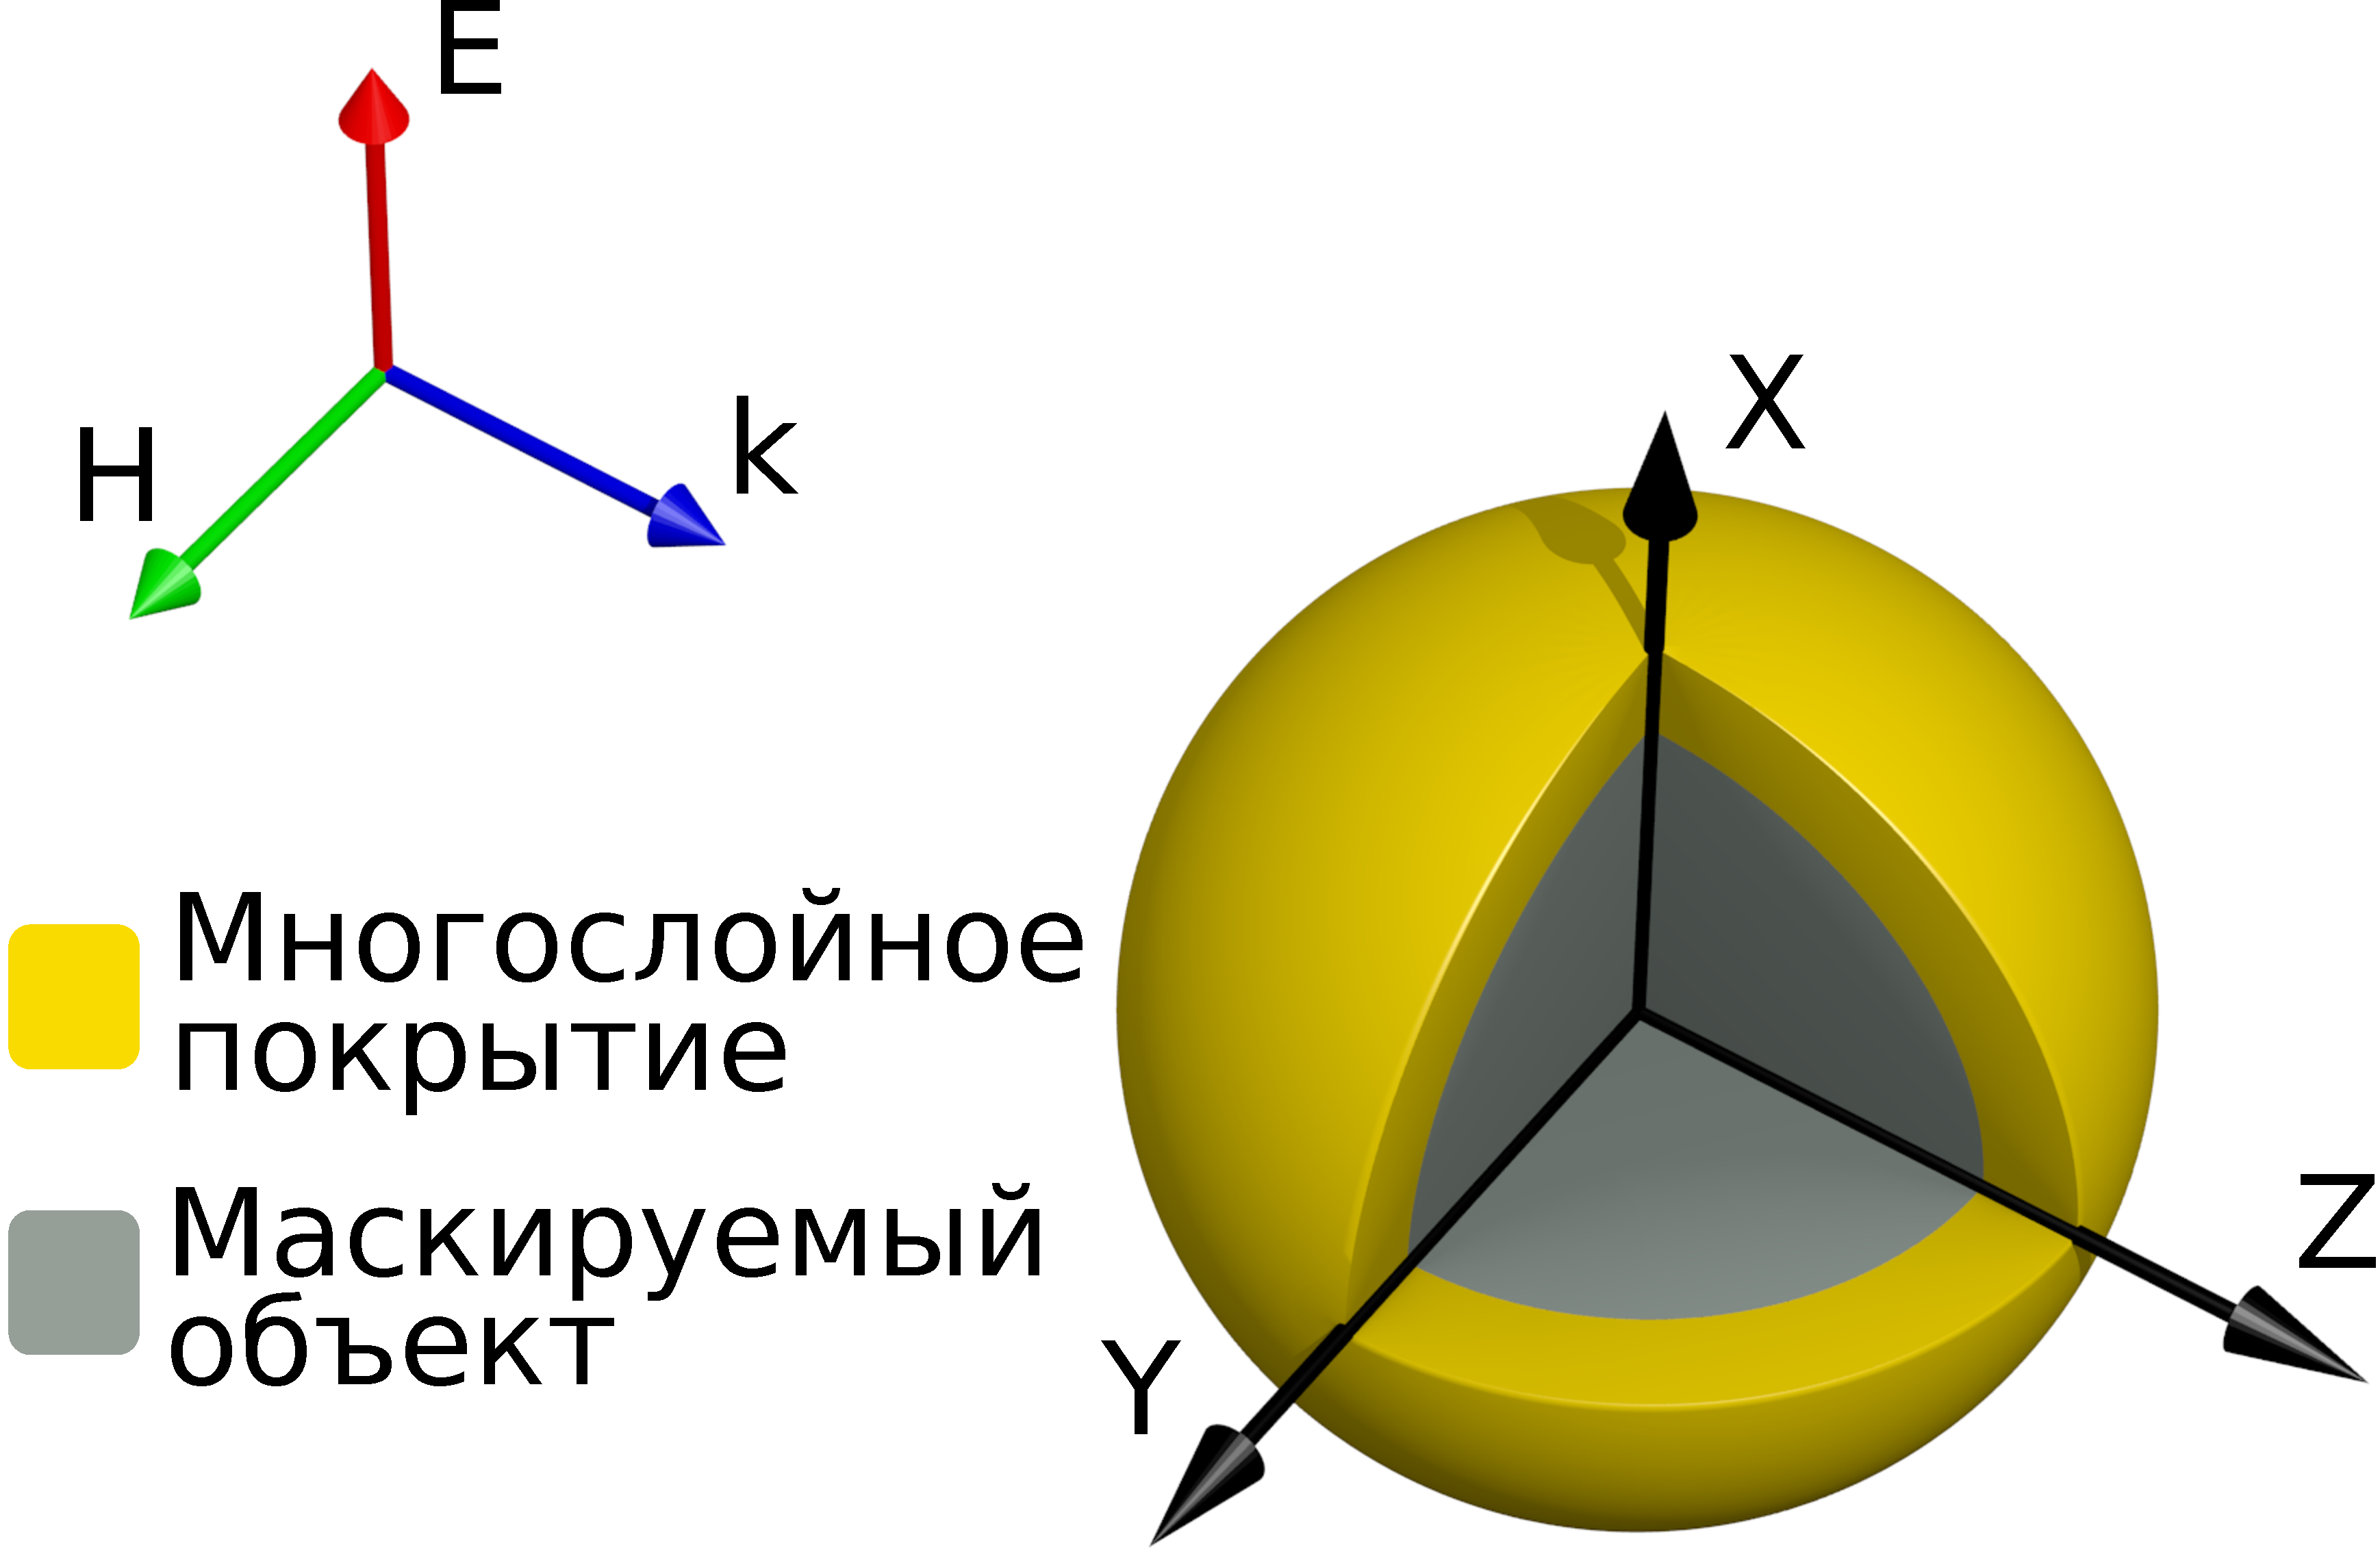
\includegraphics[width=0.57\linewidth]{model-view}}
  \end{minipage}\\
  \vfill
  \begin{minipage}[ht]{0.99\linewidth}
    \centering{а)}
  \end{minipage}\\
  \vfill
  \begin{minipage}[ht]{0.99\linewidth}
    \centering{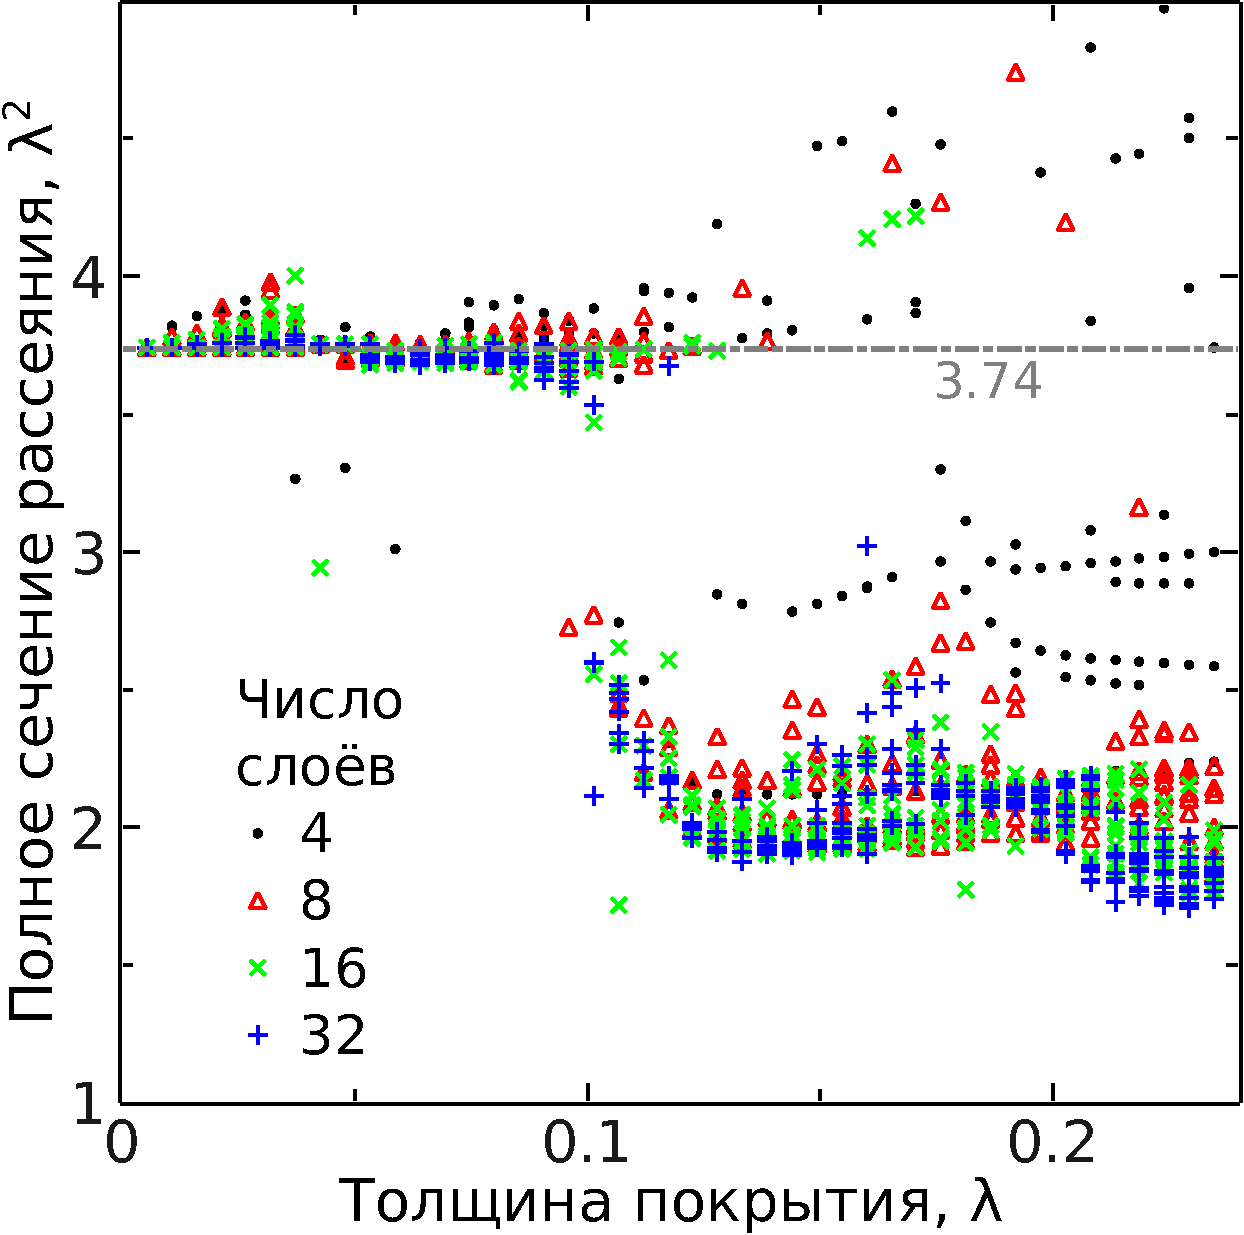
\includegraphics[width=0.57\linewidth]{rcs-overview}}
  \end{minipage}\\
  \vfill
  \begin{minipage}[ht]{0.99\linewidth}
    \centering{б)}
  \end{minipage}
  \vfill

  \caption{(a) Схематическое изображение изучаемой системы:
    маскируемый объект -- сфера из идеального проводящего материала
    внутри многослойного диэлектрического покрытия и падающая
    электромагнитная волна. (б)~Результат работы оптимизатора для
    объекта диаметром $1.5\lambda$.  Каждая отметка на графике
    соответствует одному дизайну покрытия, полученному в результате
    минимизации рассеяния. При толщине покрытия $>0.15\lambda$
    рассеяние можно уменьшить в $\sim 2$ раза.}
  \label{img:scattering}  
\end{figure}

\begin{figure}[p]
  \begin{minipage}[ht]{0.99\linewidth}
    \centering{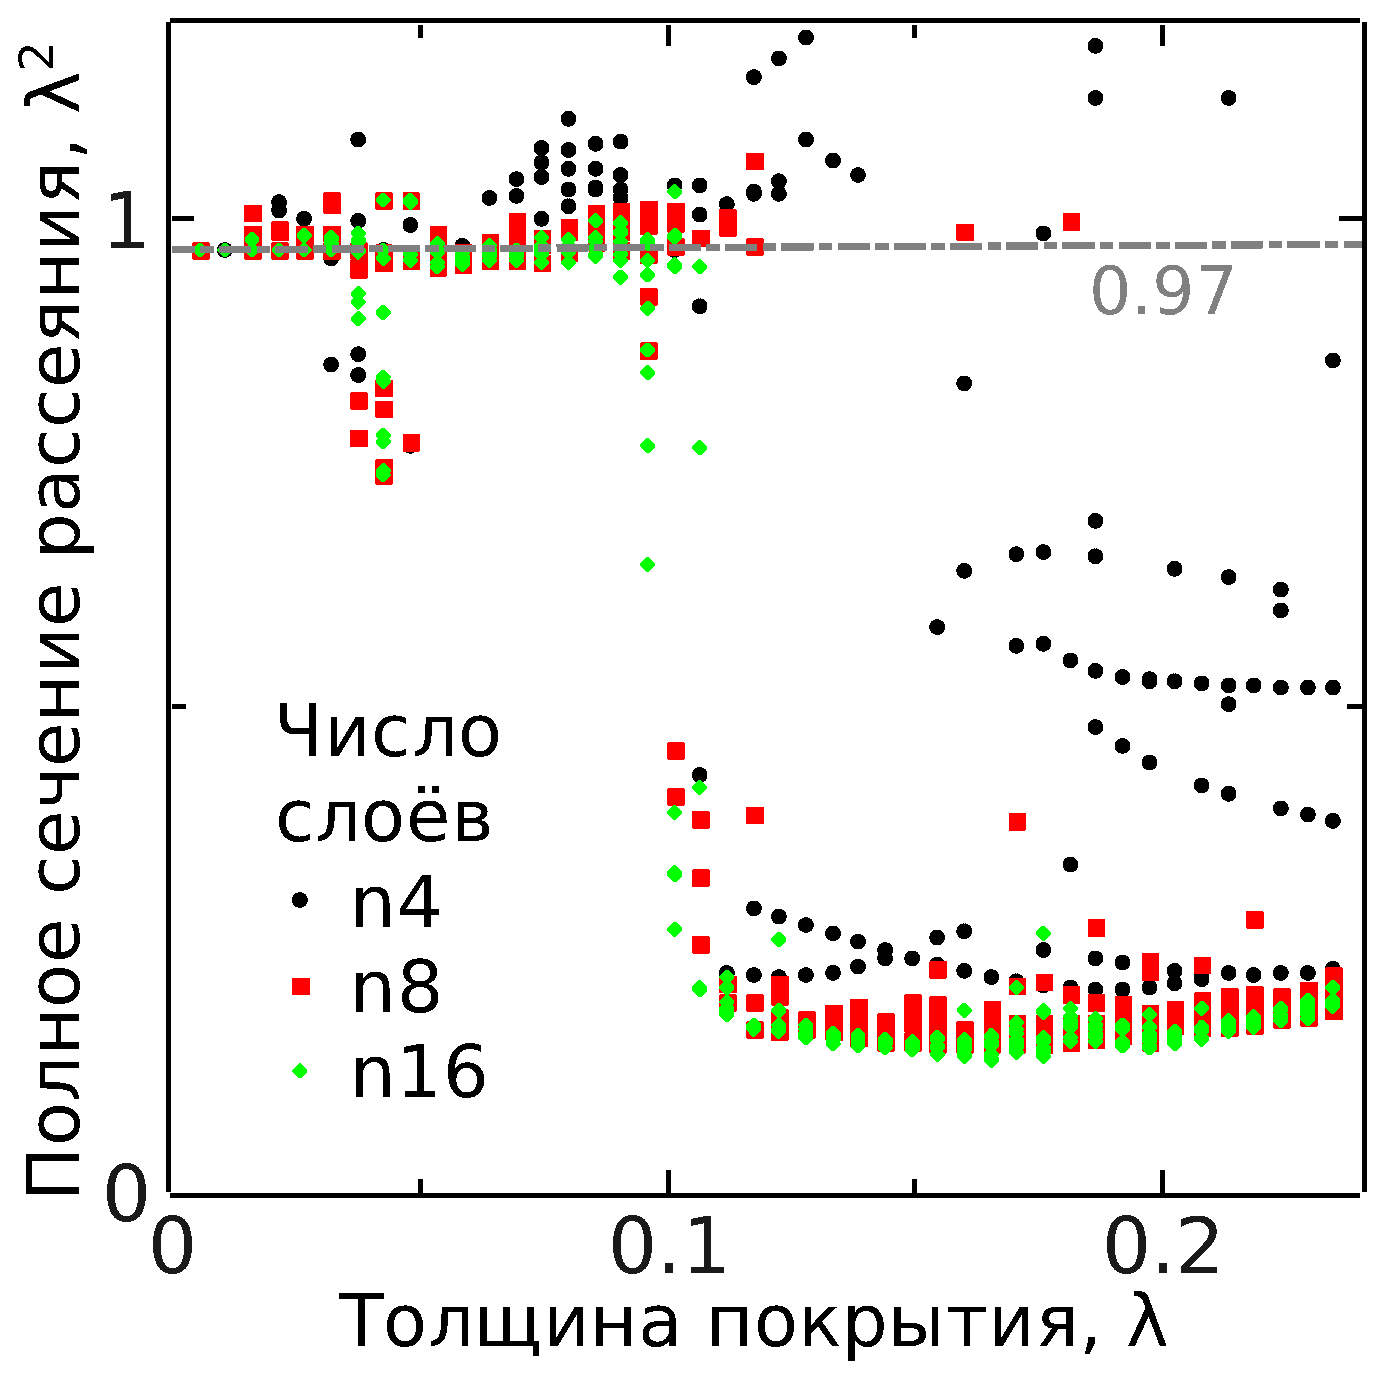
\includegraphics[width=0.57\linewidth]{rcs-overview-r14}}
  \end{minipage}\\
  \begin{minipage}[ht]{0.99\linewidth}
    \centering{а)}
  \end{minipage}\\
  \vfill
  \begin{minipage}[ht]{0.99\linewidth}
    \centering{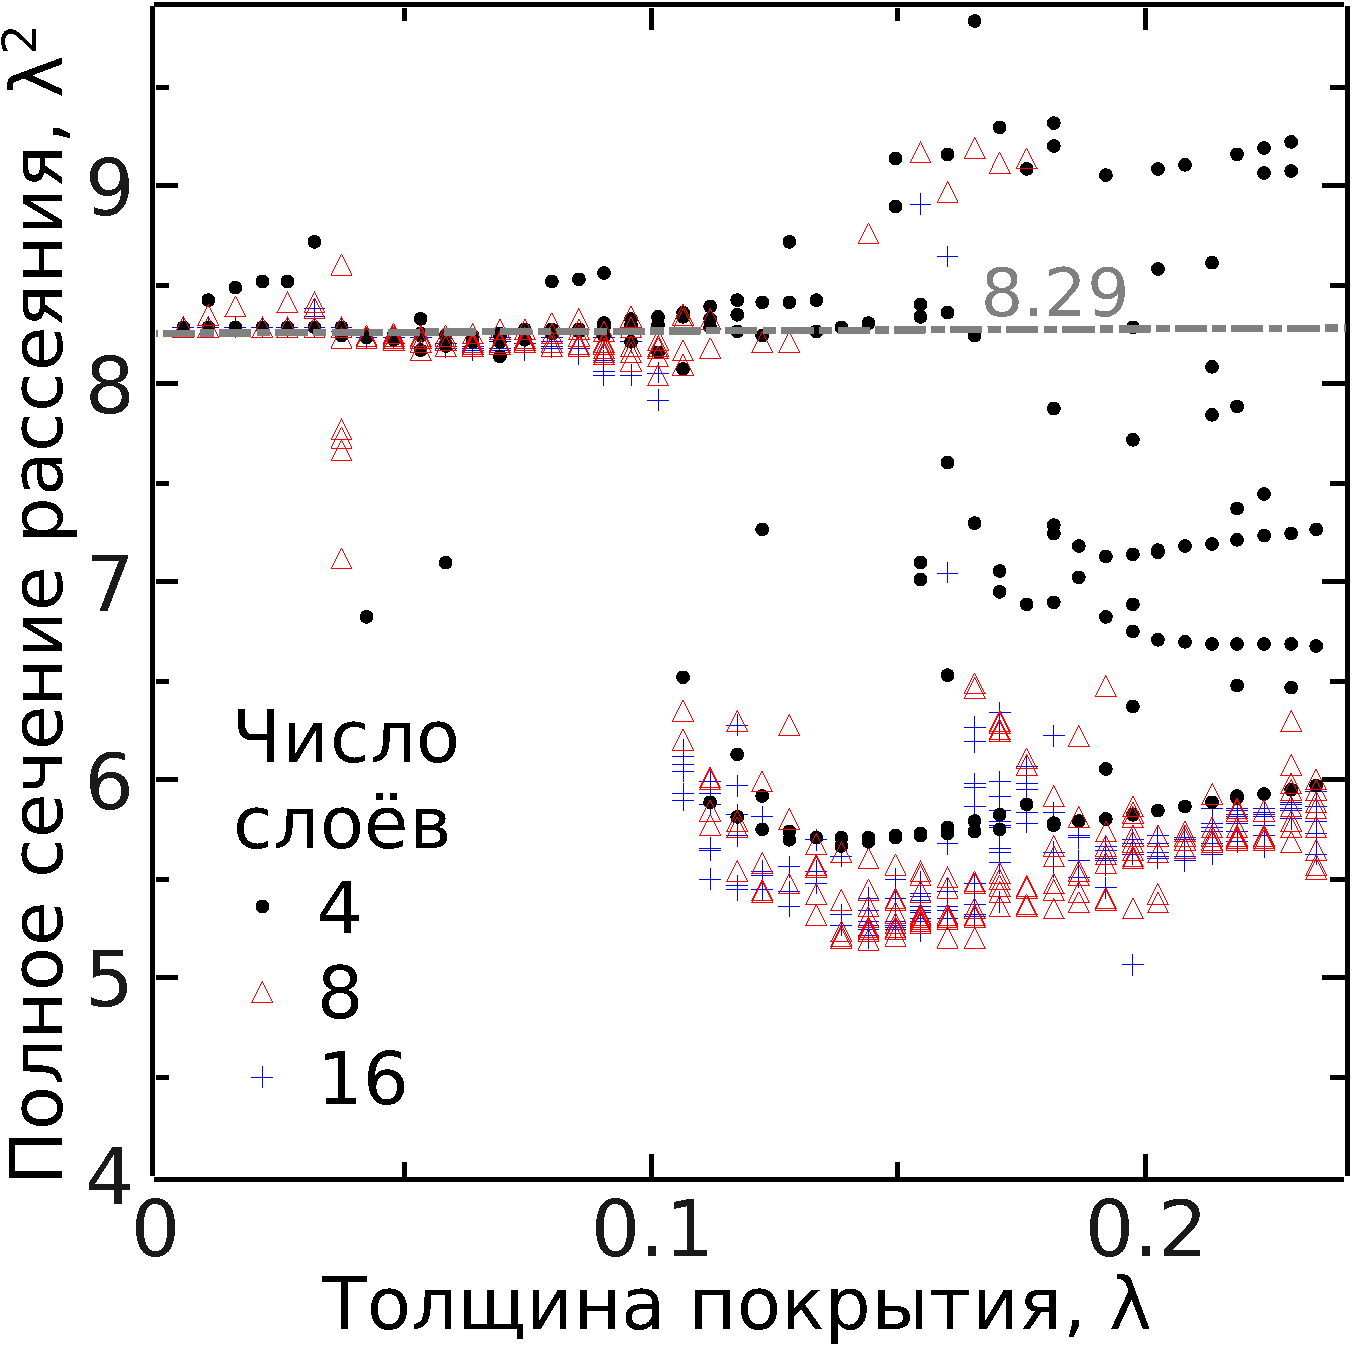
\includegraphics[width=0.57\linewidth]{rcs-overview-r42}}
  \end{minipage}\\
  \begin{minipage}[ht]{0.99\linewidth}
    \centering{б)}
  \end{minipage}
  \vfill
  \caption{Аналогично Рис.~\ref{img:scattering}(б), но для мишени
    (a)~${R_2 = 0.38\lambda}$ и (б)~${R_3 = 1.1\lambda}$.  Типичное
    значение уменьшения TSCS составило приблизительно -85\% и -35\%
    соответственно.  \label{img:rcs-overview-r14-42}}%
\end{figure}


Результат оптимизации в виде зависимости полного сечения рассеяния от
количества слоёв и общей толщины покрытия приводится на
рисунке~\ref{img:scattering}(б) и
рисунках~\ref{img:rcs-overview-r14-42}(а-б). Возможное снижение TSCS
было проверено для разных толщин покрытия в диапазоне от
${W = 0.005\lambda}$ до ${W = 0.235\lambda}$ с шагом $0.005\lambda$ с
помощью серии проходов оптимизации. Были протестированы случаи
разбиения покрытия на 4, 8, 16 (для всех радиусов) и 32 слоя (для
радиуса среднего размера). На рисунках хорошо видно, что существует
некоторое критическое значение для общей толщины покрытия
(${{\rmfamily W}\approx 0.1\lambda}$), до которого дизайнов с
пониженной TSCS относительно непокрытой мишени практически
нет. Большинство дизайнов с пониженной TSCS, обнаруженных
оптимизатором, имеют толщину покрытия выше критической.


Рассмотрим более подробно случай радиуса мишени ${R_1 =
  0.75\lambda}$. Типичное снижение TSCS относительно непокрытой мишени
для толщины выше критической составляет ${\approx -50\%}$ (в два раза
ниже). Непосредственно после превышения критической толщины
превалируют однодолинные
дизайны~(Рис.~\ref{img:designs}(а), на всех графиках
дизайнов в настоящей статье мишень, представленная PEC сферой,
расположена слева, а открытое пространство справа).
\begin{figure}[p]
  \hfill
  \begin{minipage}[ht]{0.44\linewidth}
    \centering{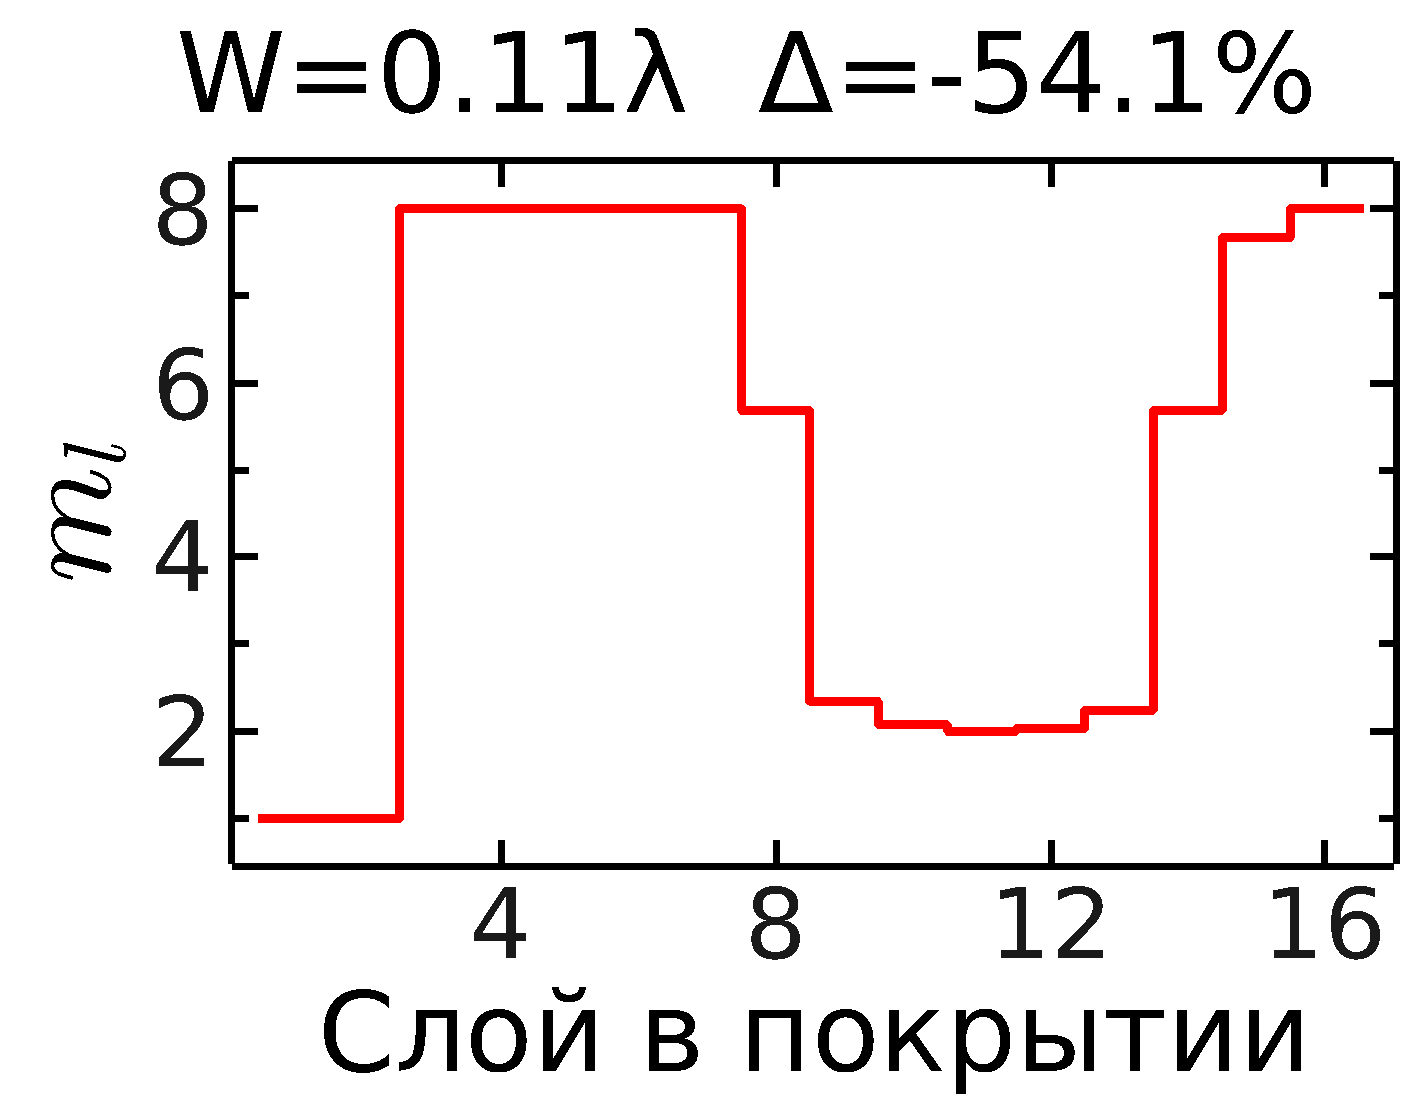
\includegraphics[width=0.95\linewidth]{w04-single-valley-index} \\ а)}
  \end{minipage}
  \hfill
  \begin{minipage}[ht]{0.44\linewidth}
    \centering{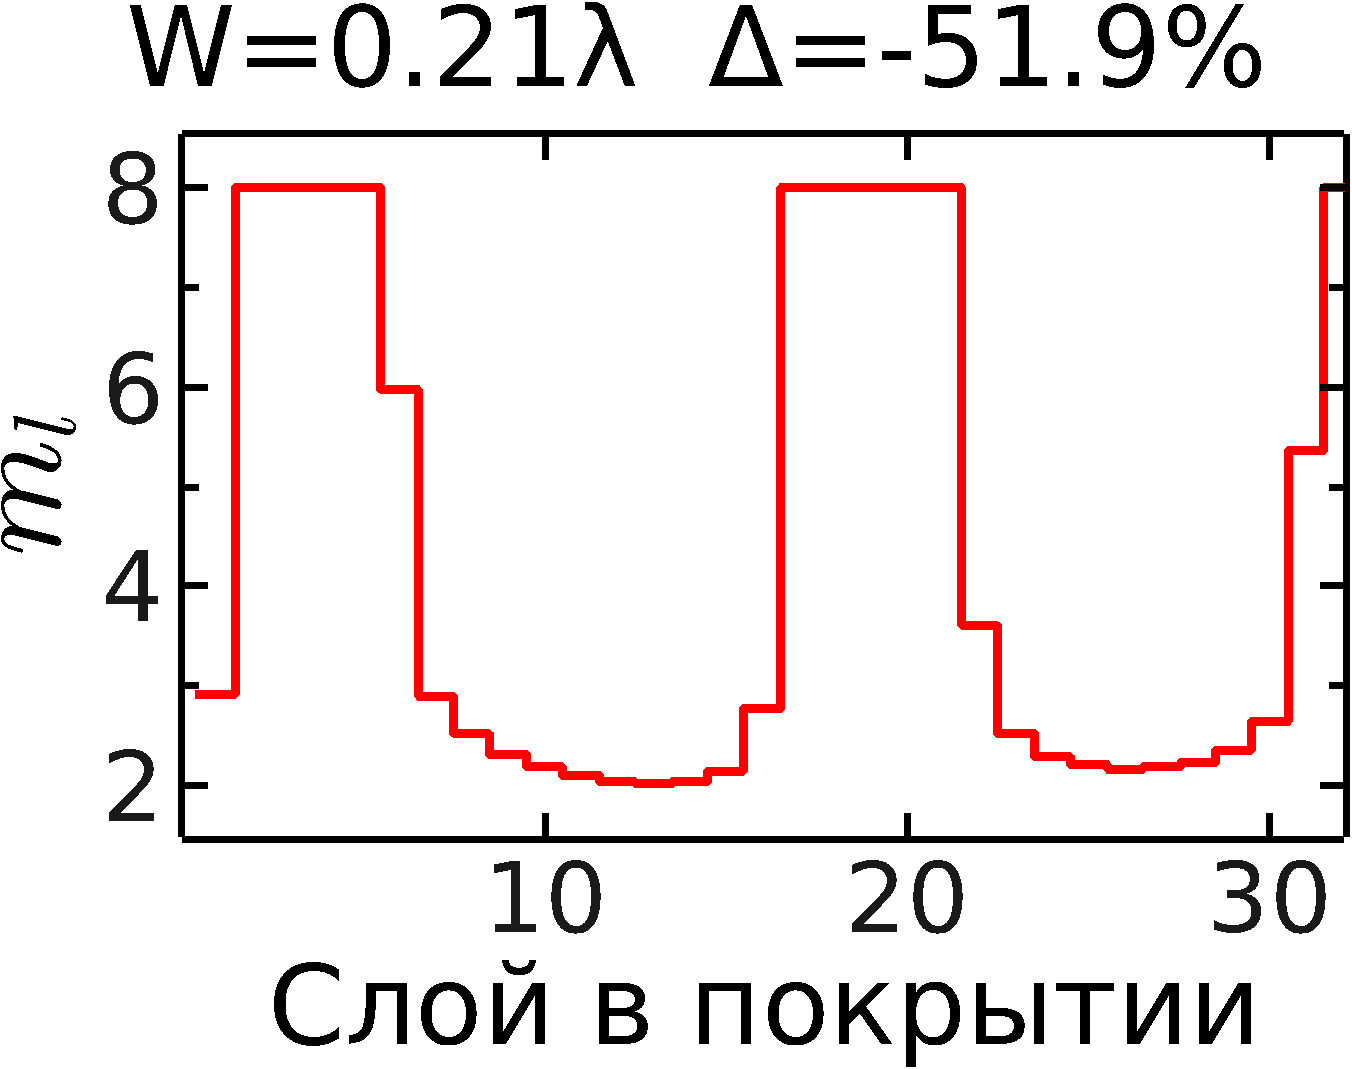
\includegraphics[width=0.95\linewidth]{w08-double-valley-index} \\ б)}
  \end{minipage}
  % \begin{minipage}[ht]{0.32\linewidth}
  %   \centering{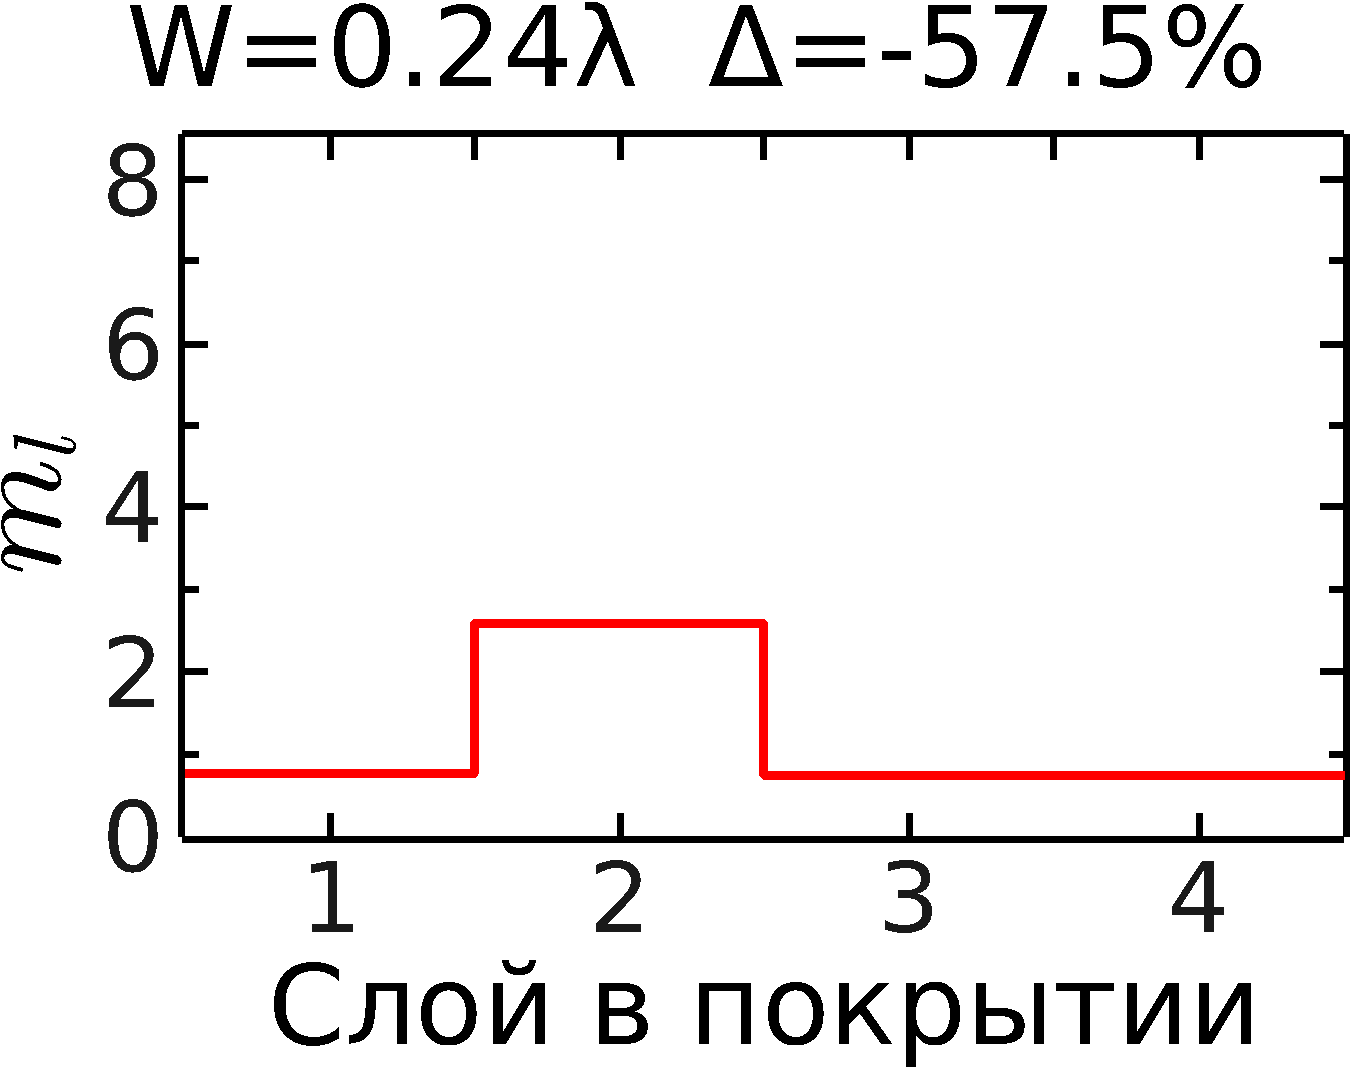
\includegraphics[width=0.95\linewidth]{index07-TO} \\ в)}
  % \end{minipage}
  \caption{Типичные дизайны, обеспечивающие наилучшую маскировку при
    толщине покрытия, равной (a)~$0.11\lambda$ и
    (б)~$0.21\lambda$. Максимальное значение показателя преломления
    было ограничено $n_{\mathrm{max}}=8$, а минимальное значение было
    равно $n_{\mathrm{min}}=1$ }
  \label{img:designs}  
\end{figure}
\begin{figure}[p]
  \begin{minipage}[ht]{0.495\linewidth}
    \centering{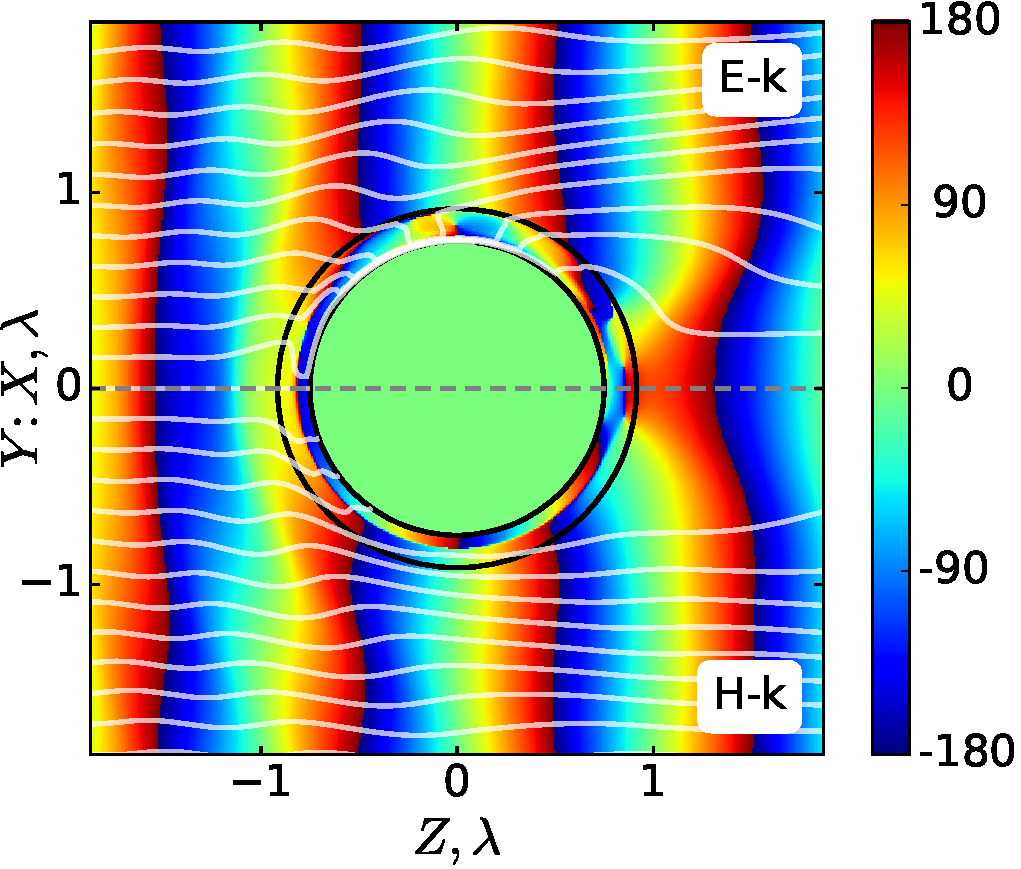
\includegraphics[width=0.98\linewidth]{PEC-index-sv-R3-XYZ-angleEx} \\ а)}
  \end{minipage}
  \hfill
  \begin{minipage}[ht]{0.495\linewidth}
    \centering{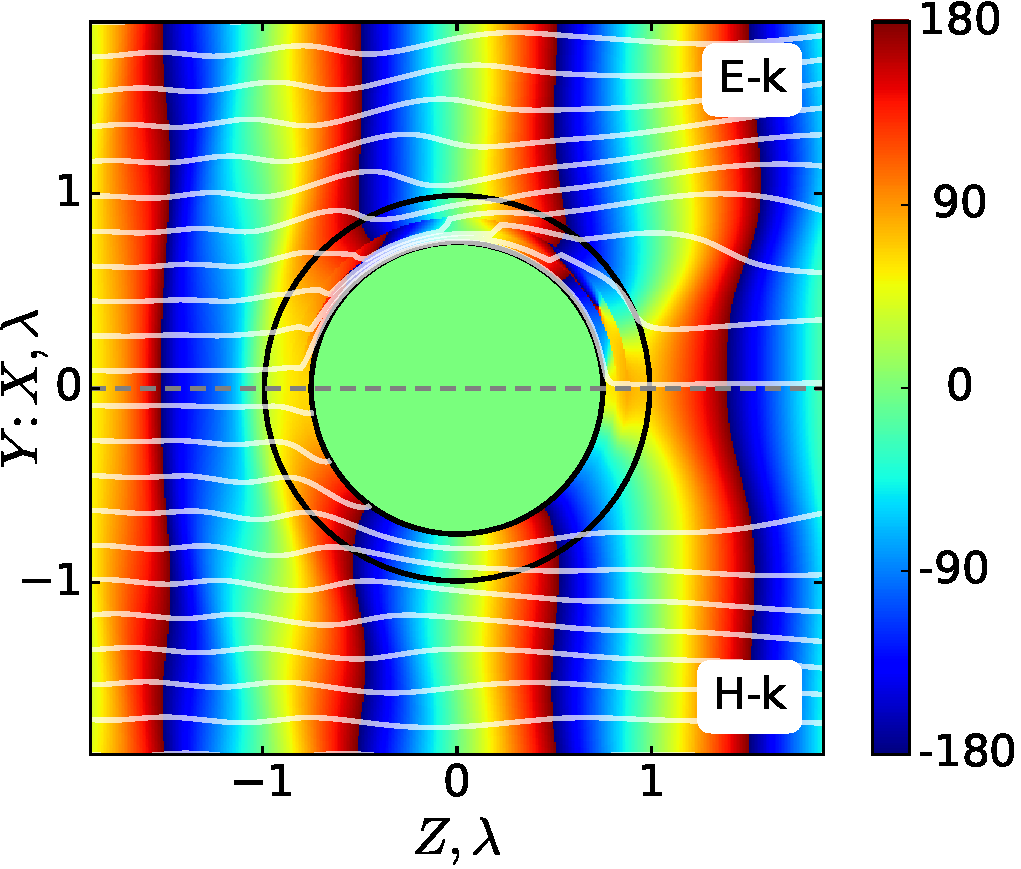
\includegraphics[width=0.98\linewidth]{PEC-index-in-glass-R1-XYZ-angleEx} \\ б)}
  \end{minipage}
  \caption{Изображение фазы электрического поля в случае маскировки
    объекта покрытием из изотропных (а) диэлектриков
    (см.~рисунок~\ref{img:designs}(а)) и (б) материалов с
    ${\varepsilon <1}$ (см.~рисунок~\ref{img:designs}(в)). Изображения
    построены в виде эпюра из плоскости поляризации падающей волны
    (верхняя половина) и перпендикулярной плоскости (нижняя
    половина). Чёрные окружности маркируют границы маскирующего
    покрытия. Белым обозначены линии потока энергии, волна
    распространяется в плоскости рисунка слева направо.}
  \label{img:field-phase}  
\end{figure}
Такие дизайны, как правило, начинаются с воздушного промежутка между
покрытием и мишенью из PEC, затем следует быстрое увеличение
показателя преломления до максимально допустимого. После нескольких
слоёв с высоким значением величина показателя преломления постепенно
идёт вниз и снова вверх, образуя долину с низким значением внутри двух
стенок с высоким значением. Минимальное значение показателя
преломления в долине обычно оказывается около двух. За второй стенкой
долины величина показателя преломления резко падает с высокого значения до
уровня воздуха.

Наряду с ростом толщины от ${\approx 0.62}$~см до ${\approx 0.78}$~см
происходит переход ~(Рис.~\ref{fig:transition}) от
однодолинного~(Рис.~\ref{fig:single-valley-index-design}) к
двухдолинному~(Рис.~\ref{fig:CST-index-design}) дизайну, где оба
дизайна сосуществуют при одной и той же толщине.

\begin{figure}
  \begin{minipage}[h]{0.45\textwidth}
    % W=0.62~cm $\Delta$TSCS=-47.9\% \\
    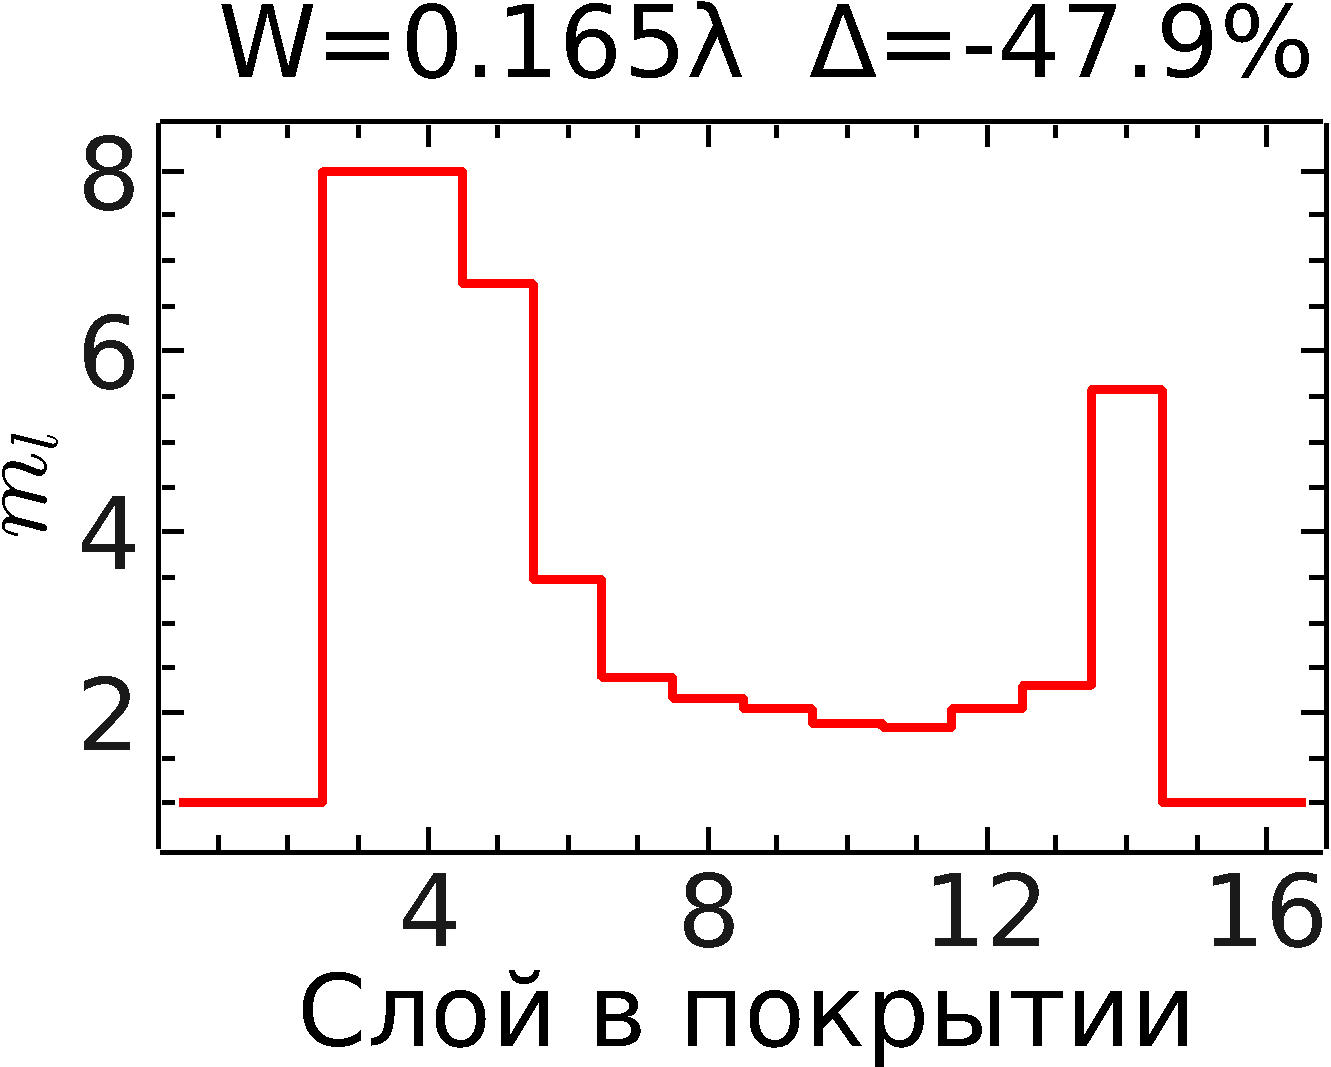
\includegraphics[width=0.99\textwidth]{w062-s-diff-479}
  \end{minipage}
  \hfill
  \begin{minipage}[h]{0.45\textwidth}
    % W=0.62~cm $\Delta$TSCS=-32.3\%\\
    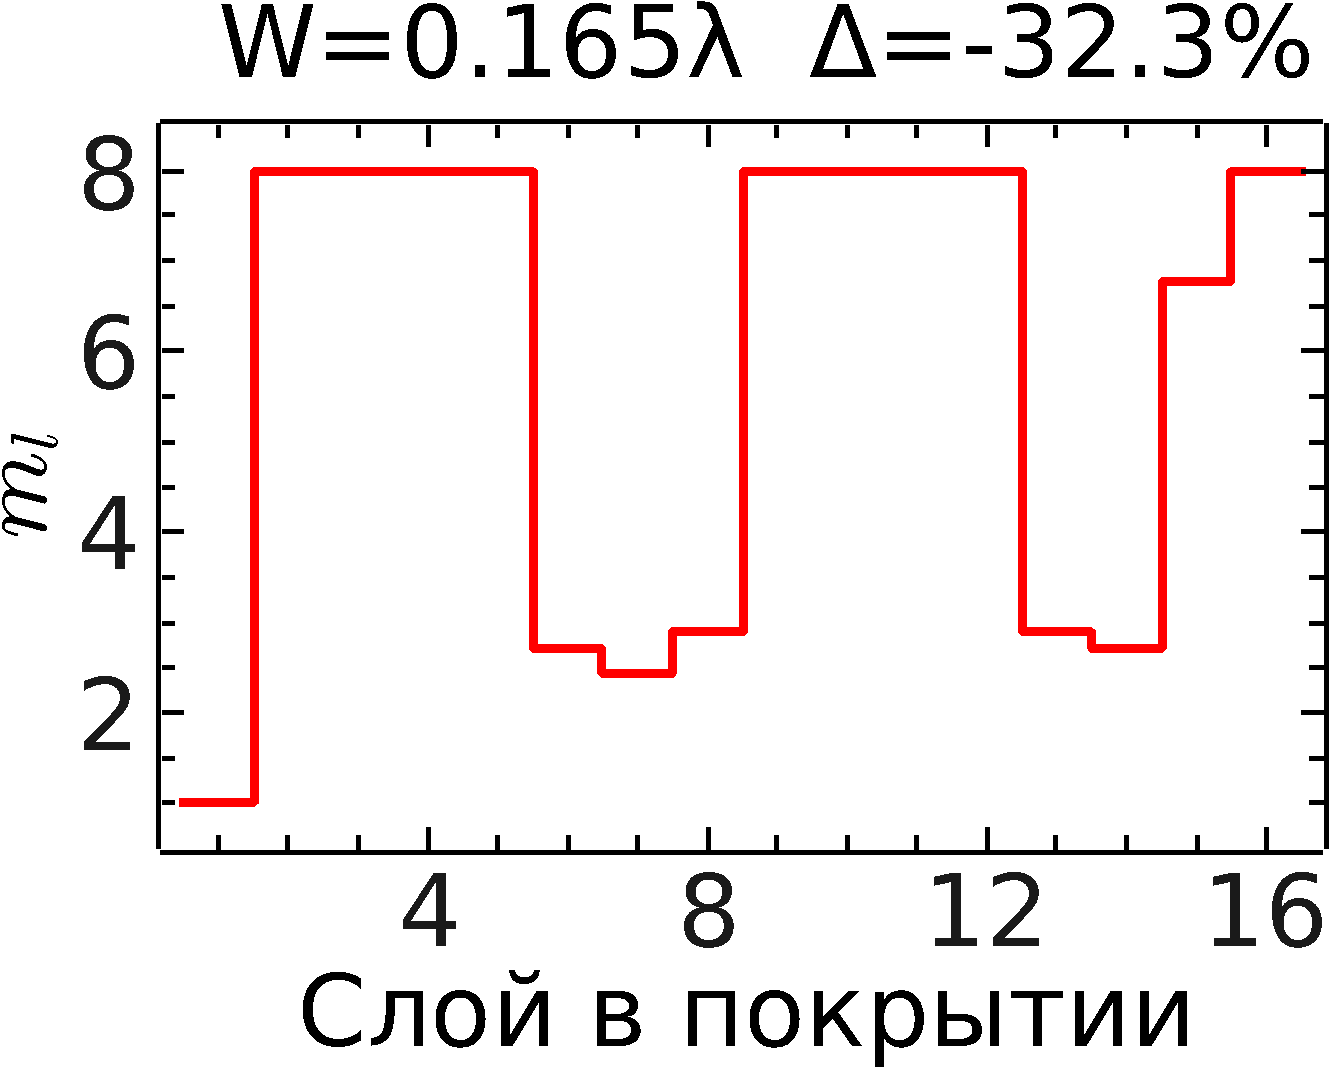
\includegraphics[width=0.99\textwidth]{w062-t-diff-323}
  \end{minipage}\\
  \vspace{12pt}\\
  % \vfill
  \begin{minipage}[h]{0.45\textwidth}
    % W=0.76~cm $\Delta$TSCS=-46.9\%\\
    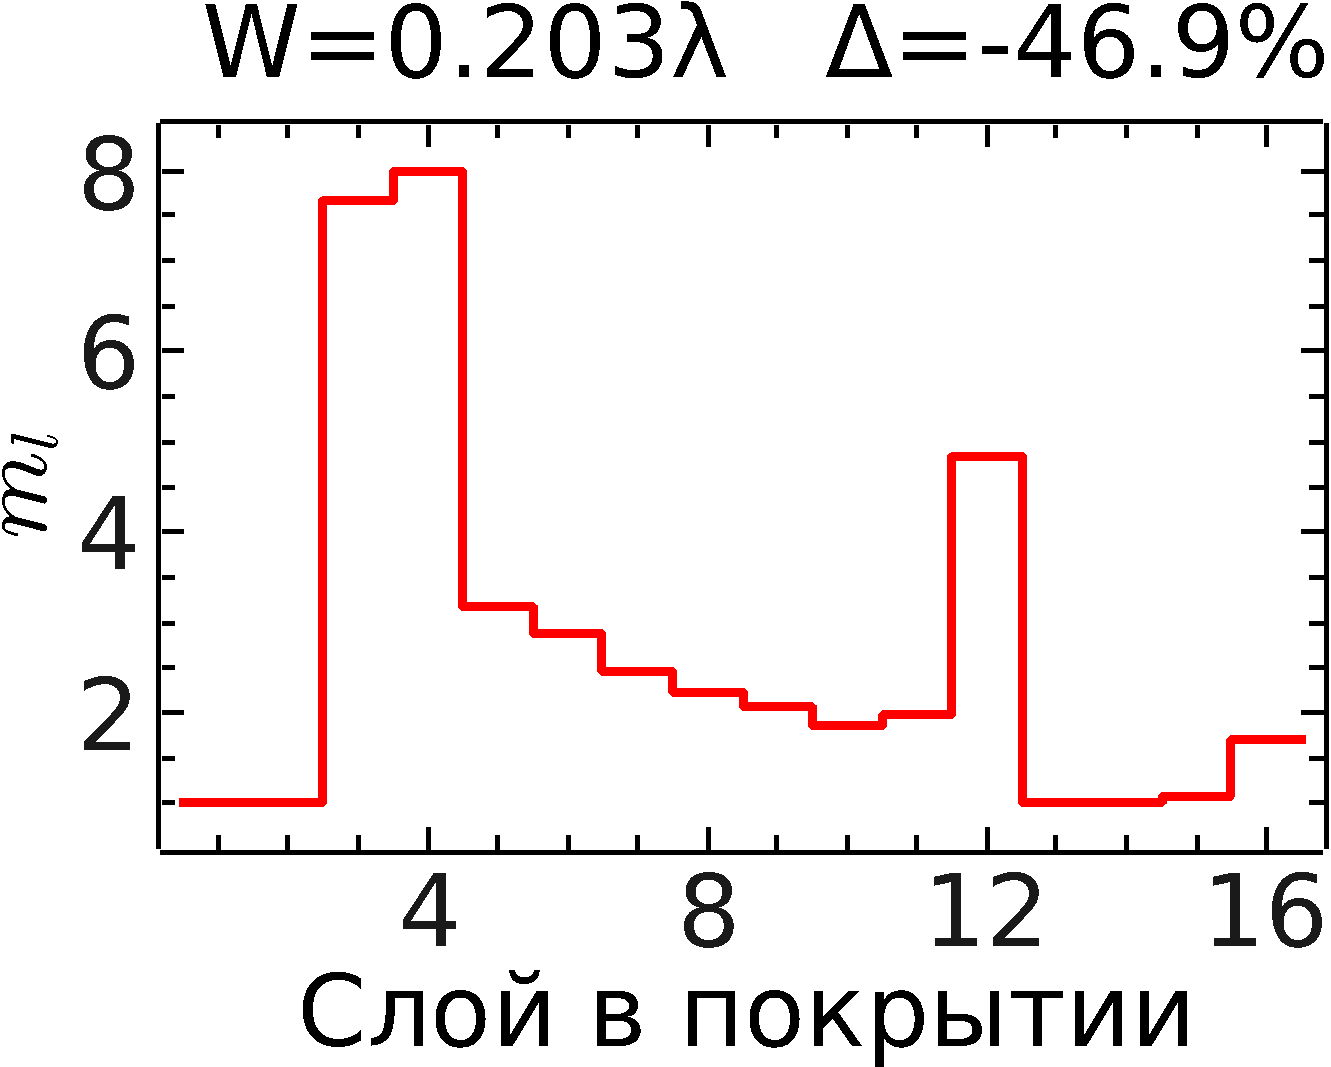
\includegraphics[width=0.99\textwidth]{w076-s-diff-469}
  \end{minipage}
  \hfill
  \begin{minipage}[h]{0.45\textwidth}
    % W=0.76~cm $\Delta$TSCS=-41.9\%\\
    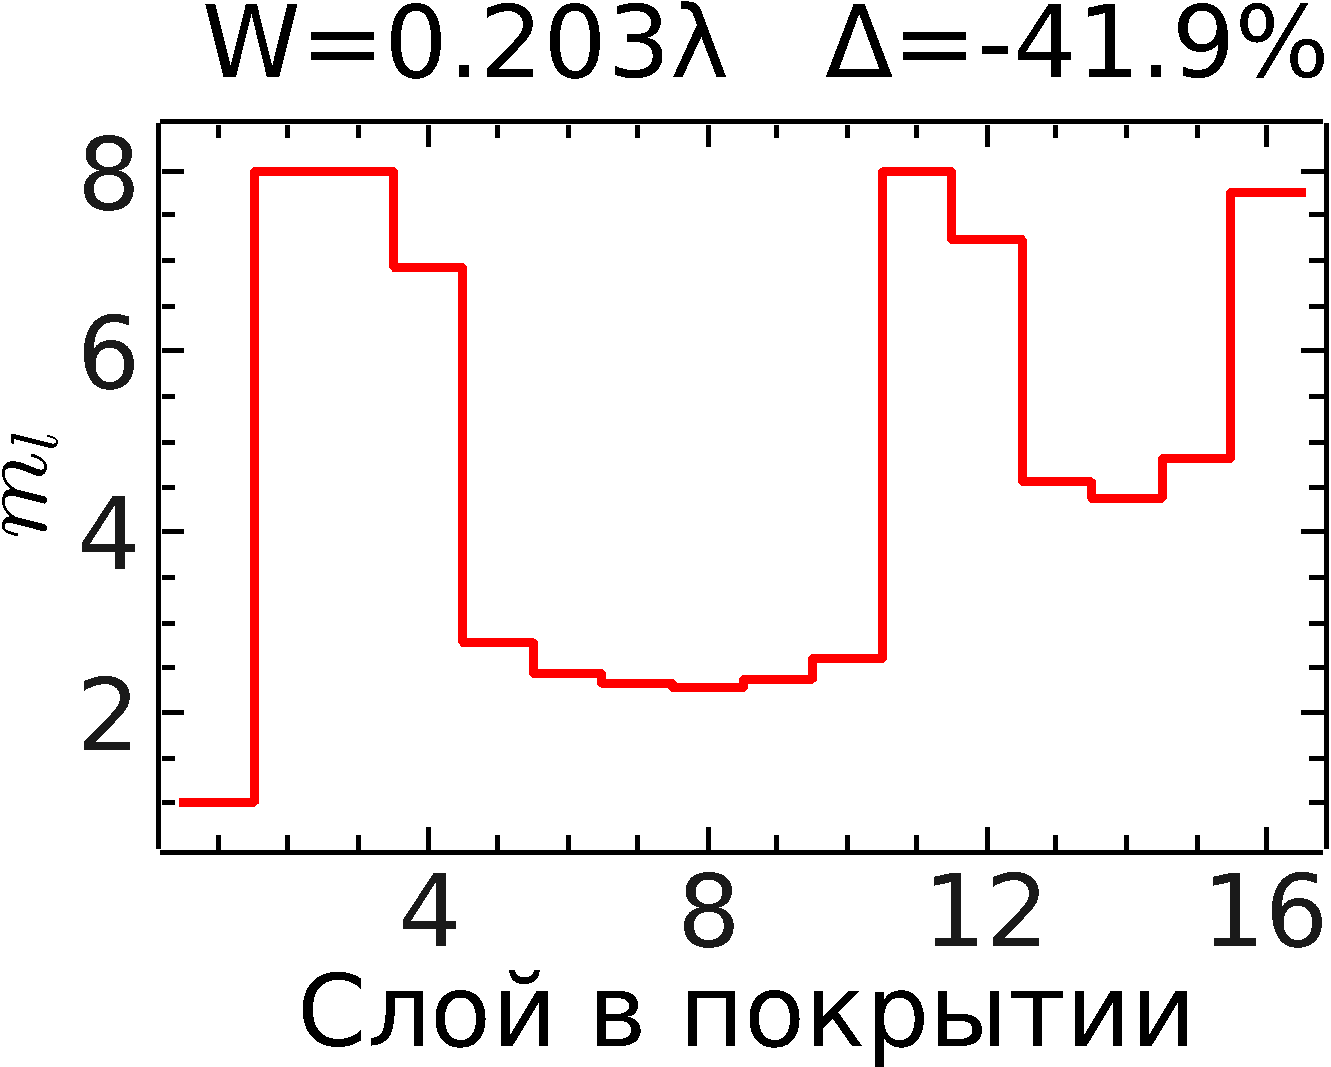
\includegraphics[width=0.99\textwidth]{w076-t-diff-419}
  \end{minipage}%
  \caption{Переход от однодолинного к двухдолинному дизайну. Каждый
    профиль показателя преломления был получен в отдельном проходе оптимизации.
    \label{fig:transition}}%
\end{figure}
Для толщины покрытия более ${\approx 0.68}$~см большинство дизайнов
имеет двухдолинную конфигурацию, немногие остальные не в полной мере
соответствуют однодолинной модели из-за наличия в покрытии внутреннего или
внешнего слоя с относительно высоким значением показателя
преломления. Для толщины выше ${\approx 0.78}$~м однодолинных дизайнов
обнаружено не было.

Во время перехода однодолинный дизайн представляется довольно
стабильным, поскольку он достиг наилучшего состояния. Двухдолинный
дизайн, видимо, ограничен допустимой толщиной покрытия. С увеличением
толщины покрытия ширина долин также увеличивается. Ширина внутренней
долины (которая ближе к PEC мишени) растёт быстрее. Это может быть
связано со следующим фактом: электромагнитное поле в покрытии в
основном сосредоточено во внутренних слоях
(Рис.~\ref{fig:CST-Ex}). Таким образом, дизайн внутренних слоёв
оказывает более сильное воздействие на итоговую TSCS по сравнению с
наружными слоями; следовательно, внутренние слои имеют приоритет при
оптимизации.

Существенного дополнительного снижения TSCS после перехода
не наблюдается. Мы полагаем, что также возможны многодолинные дизайны;
однако мы не смогли получить их из-за ограничений по времени и по
вычислительным мощностям. Была проведена быстрая попытка оптимизации
для толщины покрытия 2.4~см, для которой оптимизатор смог найти некий
дизайн~(Рис.~\ref{fig:thick}) с 54.3\% падением TSCS.
\begin{figure}
  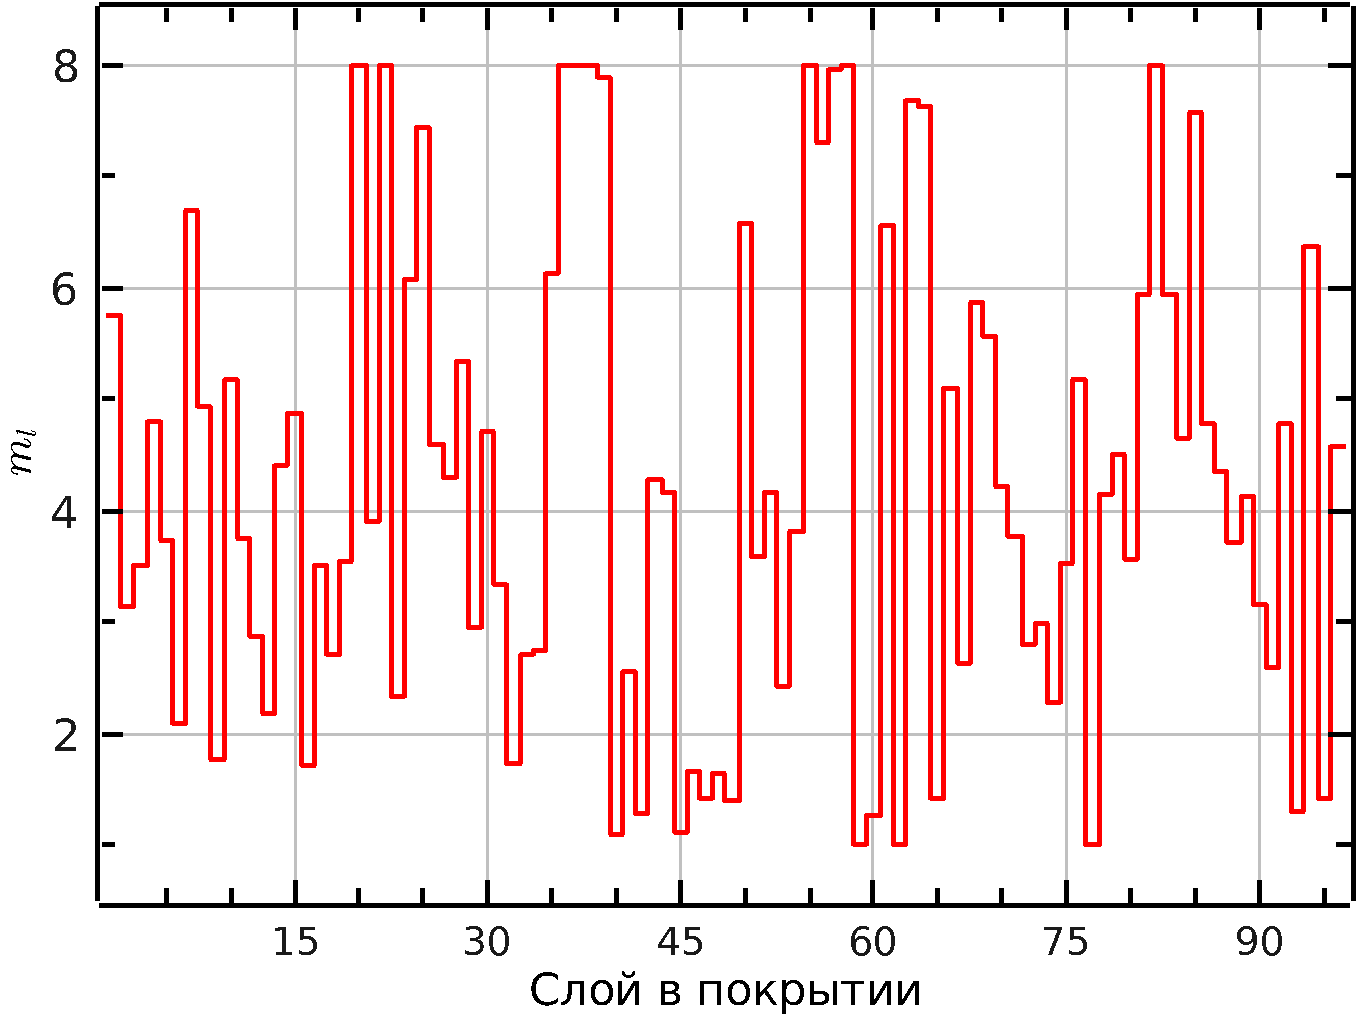
\includegraphics[width=0.47\textwidth]{w24-chaotic-index}%
  \caption{Хаотический дизайн для толщины покрытия $W=2.4$~cm
    $\Delta =-54.3$\% после 10~000 поколений.
    \label{fig:thick}}%
\end{figure}
К сожалению, он выглядит довольно хаотично и не поддаётся простой
классификации.

%БЛОК 2

Необходимо отметить, что <<дёрганое>> поведение профиля показателя
преломления, хорошо видное в случае хаотического дизайна, может быть
частично обнаружено в случаях однодолинного и двухдолинных дизайнов,
описанных выше.  Это можно объяснить следующим образом: толщина
отдельного слоя внутри покрытий в десятки раз меньше длины волны (слои
являются субволновыми).  Таким образом, если поменять местами два
соседних слоя, то эффективное значение показателя преломления
поменяется слабо, и будет наблюдаться сопоставимая величина падения
TSCS.  В случае, если разница в величине показателя преломления между
этими слоями оказывается достаточно большой, то будет наблюдаться
<<дёрганое>> поведения профиля показателя преломления.  Подобное
поведение тонких многослойных покрытий представляет
существенную сложность для любого алгоритма оптимизации, так как очень
похожие друг на друга с физической точки зрения системы оказываются
сильно удалены друг от друга в многомерном пространстве входных
параметров.  Иначе говоря, у целевой функции, используемой в качестве
критерия оптимизации, наблюдаются многочисленные локальные
минимумы.  Этот факт при использовании стохастического оптимизатора
приводит к тому, что конечный результат каждого прохода может
оказаться немного другим.  По этой причине для каждого набора входных
параметров выполнялась серия проходов оптимизации, а это, в свою
очередь, обусловило наличие нескольких отметок одного типа
(одно и то же количество слоёв в покрытии) для каждой исследованной
толщины покрытия~(Рис.~\ref{fig:rcs-overview},%
~\ref{fig:rcs-overview-r14},~\ref{fig:rcs-overview-r42}), отметки с
большим значением величины TSCS обычно обладают более <<дёрганым>>
профилем показателя преломления.  В целом, несмотря на указанные
сложности, адаптивный метод дифференциальной эволюции воспроизводимо
находит дизайны  с уменьшенным рассеянием в выбранном диапазоне толщин
и числа слоёв в разбиении.

Как следует из Рис.~\ref{fig:rcs-overview}, разбиения покрытия на
четыре слоя оказывается недостаточным для достижения оптимальных
значений TSCS.  Большинство дизайнов, обладающих TSCS более 35~см$^2$ и
толщиной покрытия, превышающей критическую, используют разбиение на 4
слоя.  При этом разбиения на 8 слоёв оказывается достаточным для того,
чтобы получить результаты, сравнимые со случаями 16 и 32 слоёв
(особенно для диапазона толщин покрытия, соответствующих однодолинному
дизайну).  Тем не менее, у разбиения на 32 слоя есть небольшое
преимущество в случае большой толщины покрытия (${> 0.8}$~см).

Как было указано ранее, обнаружено небольшое число дизайнов с
маскирующим эффектом в случае толщины покрытия значительно меньше
критической.  Чтобы изучить такие дизайны мы провели дополнительную серию
оптимизаций (треугольники без заполнения на Рис.~\ref{fig:rcs-overview-thin}).
\begin{figure}
  \centering{
    % Use pdfcrop to remove white margins
    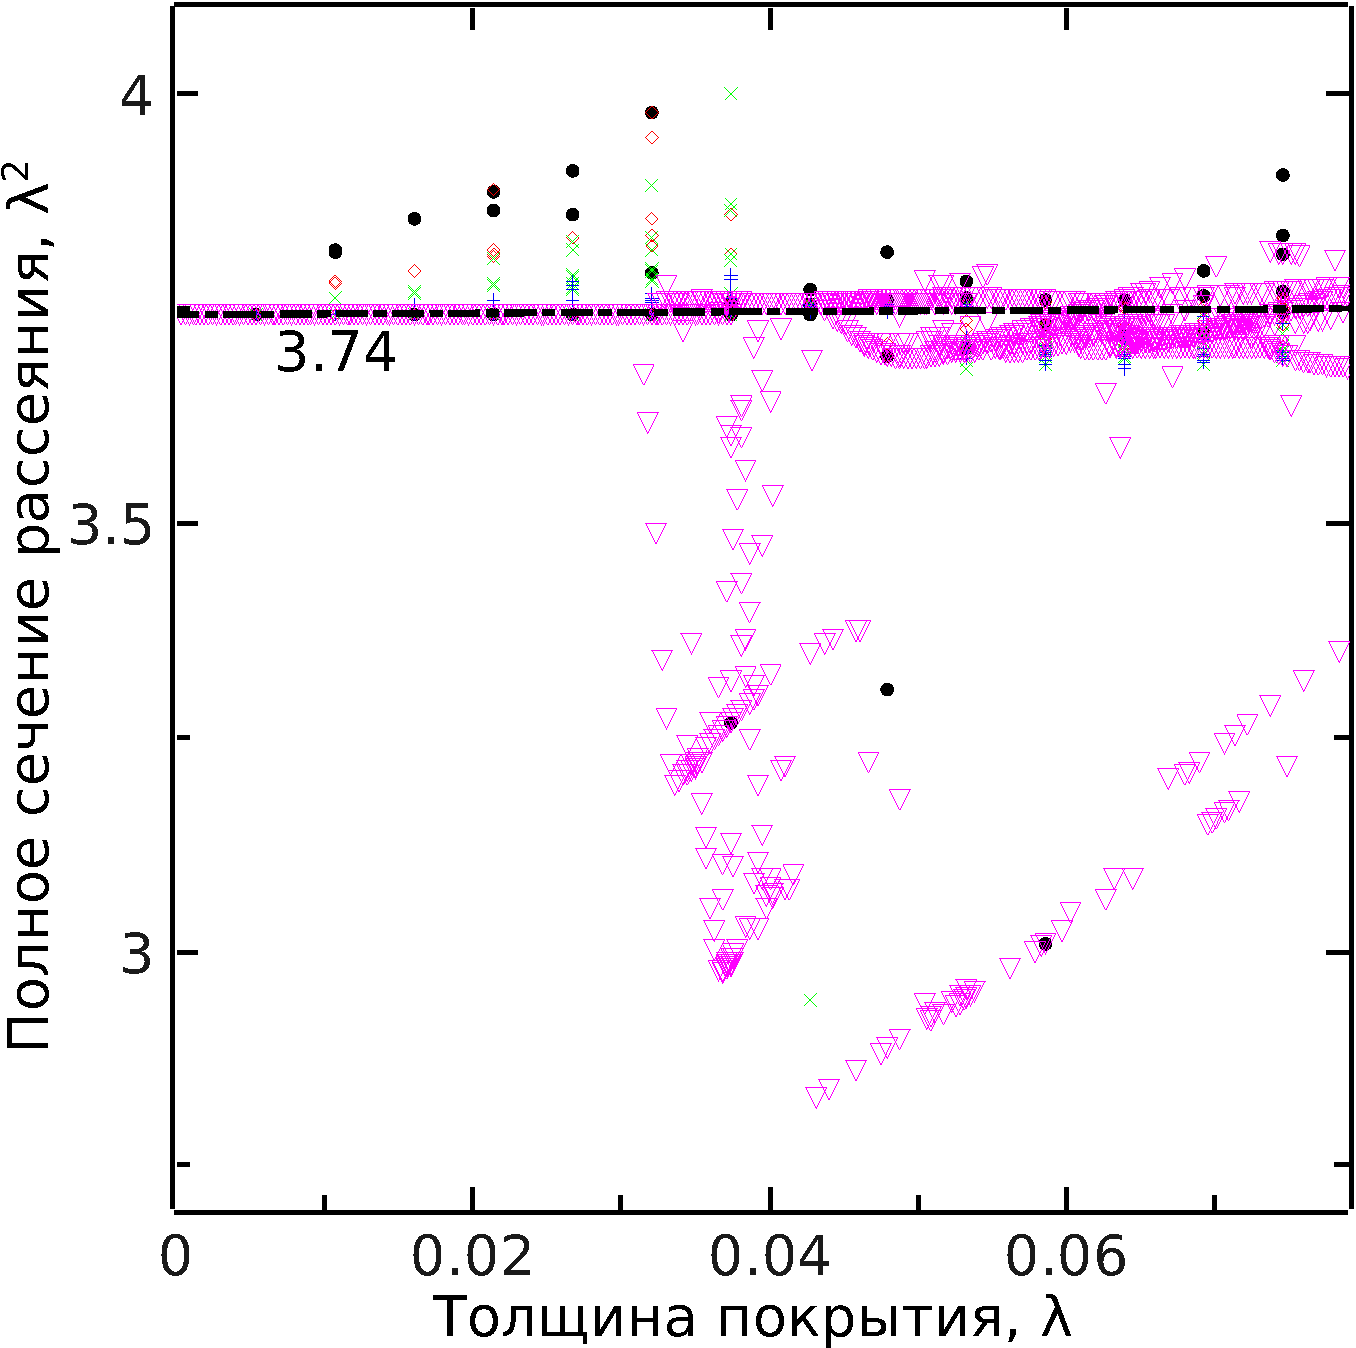
\includegraphics[width=0.47\textwidth]{rcs-overview-thin}%
      \caption{Увеличенная часть Рис.~\ref{fig:rcs-overview}) с
        дополнительными результатами оптимизации (треугольники без
        заполнения) для случая толщины покрытия меньше критической.
        Каждая отметка обозначает конечный результата одного прохода оптимизации.
        \label{fig:rcs-overview-thin}}%
  }
\end{figure}
Основываясь на ранее полученных результатах (а также по причине
ограниченных вычислительных ресурсов), мы использовали разбиение
только на 4 и 8 слоёв.  Для того чтобы добиться воспроизводимости
результатов, нам пришлось уменьшить шаг сканирования для толщины
покрытия и увеличить размер популяции в настройках оптимизатора.
Несмотря на это, всего лишь 218 проходов оптимизации из $\sim$4~000
смогли достичь значения TSCS менее 50~см$^2$.  Лучший дизайн достиг
-24\% падения TSCS для толщины покрытия 0.162~см.  Аналогичные дизайны
для сверхтонких покрытий, полученные в разных независимых прогонах
оптимизации, образуют хорошо различимые зависимости при изменении
толщины на Рис.~\ref{fig:rcs-overview-thin}.  Тем не менее, похоже, что
маскирующий эффект в таких покрытиях основан на несколько другом
физическом принципе, отличном от предлагаемого в настоящей работе, и
может быть дополнительно изучен впоследствии.

\section{Полноволновое моделирование}

Мы провели компьютерное моделирование различных дизайнов с помощью
пакета CST Microwave Studio 2013.  Полученные результаты обладают
набором общих особенностей, в иллюстративных целях мы выбрали
двухдолинный дизайн (Рис.~\ref{fig:CST-index-design}, а также его спектры Рис.~\ref{fig:CST-design-spectra}).
\begin{figure}
  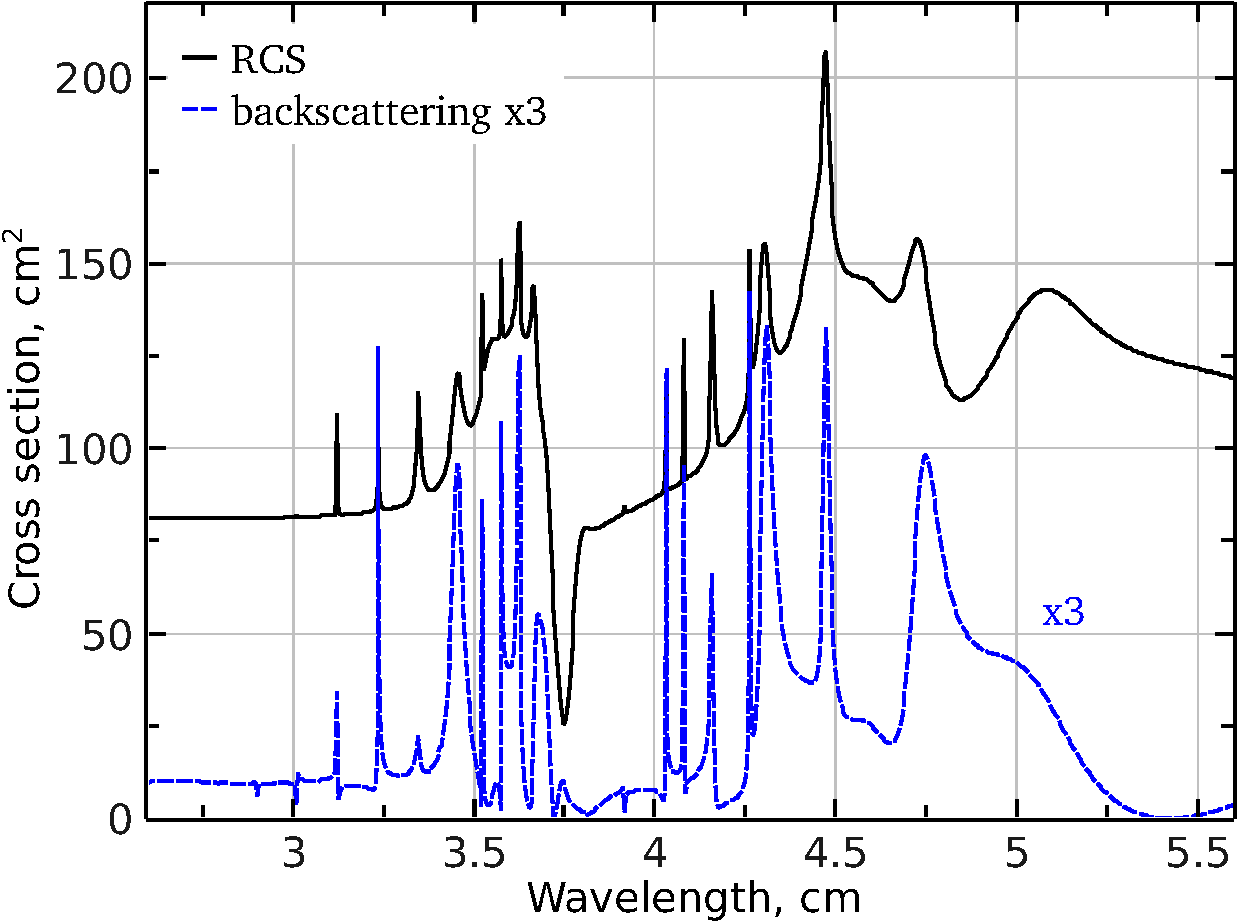
\includegraphics[width=0.47\textwidth]{w08-spectra}%
  \caption{Спектры TSCS и сечения обратного рассеяния, полученные в
    Scattnlay~\cite{Pena-scattnlay-2009} для двухдолинного дизайна,
    использованного при моделировании в пакете CST. Масштаб сечения
    для кривой обратного рассеяния увеличен в три раза.  Толщина
    покрытия $W=0.21\lambda$. Относительно непокрытой мишени $\Delta =-51.9$\%.     %TODO add    bare target spectra
    \label{fig:CST-design-spectra}}%
  % TODO Zero-backscattering can be disscused with Limonov and
  % Rybin. They can do additional review of the paper.
\end{figure}
% the CST rcs 25.4445 Mie 25.3412
Результаты компьютерного моделирования в пакете CST подтвердили
результаты расчётов с использованием теории Ми (25.44~см$^2$ и
25.34~см$^2$ соответственно).

Стационарное распределение поля (амплитуда  и фаза на
Рис.~\ref{fig:CST-Ex}) на частоте ${f = 8}$~ГГц были получены при
использовании алгоритмов CST в частотной области для разупорядоченной
тетрагональной сетки.
\begin{figure}
  \centering{
    % Use pdfcrop to remove white margins
    \begin{minipage}[h]{0.47\textwidth}
      a)\hfill
      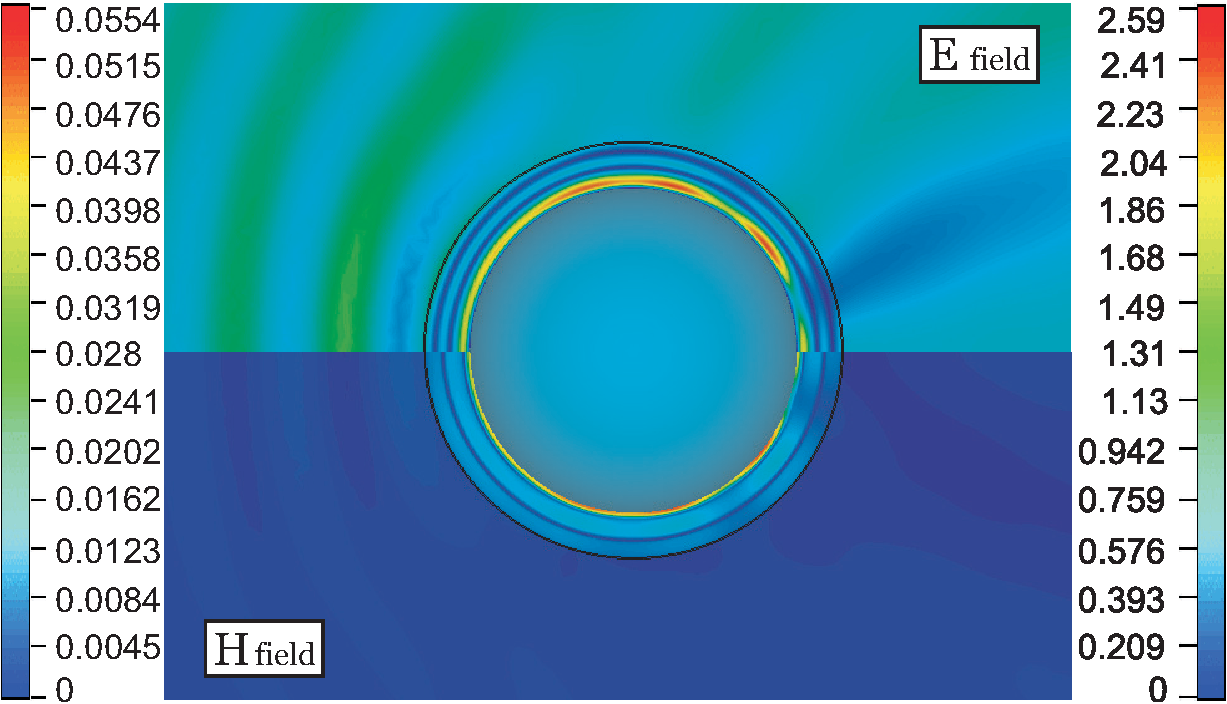
\includegraphics[width=0.95\textwidth]{W08-planeYZ-E-H-abs}%
    \end{minipage}\\%
    \begin{minipage}[h]{0.47\textwidth}
      b)\hfill
      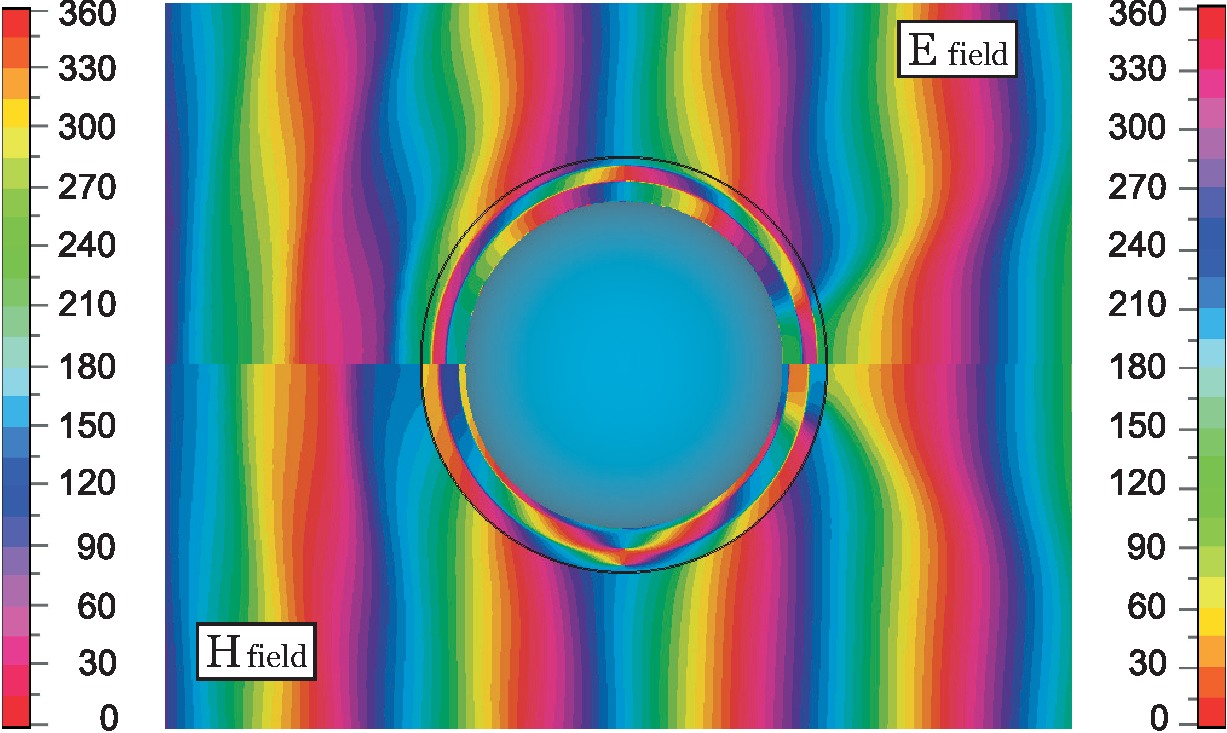
\includegraphics[width=0.95\textwidth]{W08-planeYZ-E-H-phase}%
    \end{minipage}%
      \caption{Амплитуда (a) и фаза (b) электрического (верхняя
        половина) и магнитного (нижняя половина) поля для
        двухдолинного дизайна. Окружности чёрного цвета обозначают
        границы внешнего слоя в покрытии.   Плоскость рисунка
        перпендикулярна плоскости поляризации электрического поля в
        падающей волне и проходит через центр мишени.  Амплитуда
        магнитного поля (левая шкала) измеряется в А/м, электрического
        поля (правая шкала) в В/м.  Фаза измеряется в градусах.
        \label{fig:CST-Ex}}%
  }
\end{figure}
Полное число ячеек в сетке составило около 4-х миллионов.  Для того
чтобы уменьшить моделируемый объём, мы использовали плоскости
симметрии.  Было выбрано открытое граничное условие с отражательной
способностью -40~dB.  Источник плоской волны расположен слева от
сферической мишени, плоскость поляризации электрического поля
перпендикулярна плоскости рисунка.

Необходимо отметить несколько особенностей распределения поля внутри
покрытия. 1) Электромагнитное поле в основном сконцентрировано во
внутренних слоях покрытия. 2) Присутствует нечто вроде антикорреляции
между минимумами и максимумами пространственного распределения
амплитуд электрического и магнитного полей: максимум электрического
поля соответствует минимуму магнитного и наоборот. 3) Существуют
тонкие <<переключающие>> слои с быстрым изменением фазы.  Прохождение
волны сквозь эти слои в радиальном направлении приводит к перевороту
её фазы на половину периода, далее идёт толстый слой перевёрнутой
фазы.  Положение <<переключающих>> слоёв совпадает с минимумами
амплитуды того поля, чья фаза переворачивается.

Давайте проследим за электрическим и магнитным полем, проходящим
через <<переключающие>> слои.  Такие слои можно эффективно
рассматривать как области резкого замедления распространения поля,
причиной которого является интерференция падающей и рассеянной волны.
Кроме того, плоскость постоянной фазы в области между
<<переключающими>> слоями имеет предпочтительное направление движения
в тангенциальном направлении.  Таким образом, один из возможных путей,
по которому может пойти падающая волна, выглядит следующим образом:
волна замедляется при прохождении сквозь <<переключающий>> слой, далее
она движется в радиальном направлении вдоль этого слоя,
замедляется ещё раз, проходя <<переключающий>> слой в обратном
направлении, и покидает покрытие.  Вследствие использованного дизайна
показателя преломления  набег фазы волны, проходящей внутри покрытия,
относительно волны, которая двигалась снаружи, оказывается в точности
равен полному периоду волны.  В результате поле, которое
распространялось подобным образом, не возмущает плоскость постоянной
фазы за мишенью.  Указанное поведение можно также трактовать с позиций
теории компенсации рассеяния~\cite{alu} со следующим дополнением.  В
нашем случае наличие антипараллельных векторов локальной
поляризуемости  вызвано наличием <<переключающих>> слоёв, приводящих к
изменению направления вектора электрического поля на противоположное.

В случае двухдолинного дизайна возникает два <<переключающих>> слоя.
Внешний слой работает указанным выше образом, внутренний слой работает
аналогично, но с небольшим отличием.  Набег фазы волны, проходящей
через внутренний слой, оказывается равен двум периодам.

Предложенное физическое описание механизма уменьшения полного сечения
рассеяния позволяет сделать простое предсказание.  При рассмотрении
указанных дизайнов во временной области установление стационарного
распределения амплитуды поля в области геометрической тени займёт
больше времени в случае двухдолинного дизайна по сравнению с
однодолинным.  

\section{Заключение}
Анализ этого и аналогичных графиков для других значений отношения
радиуса к длине волны~(рисунок~\ref{img:rcs-overview-r14-42}) позволил
выявить ряд характерных особенностей. Например, существует некое
пороговое значение толщины, после которого становится возможным
стабильное получение дизайнов, обеспечивающих заметное уменьшение
сечения рассеяния. При этом наилучшие показатели обеспечивают дизайны
характерной структуры, где несколько слоёв с высоким показателем
преломления окружают группу слоёв с низким показателем
преломления. Увеличение общей толщины покрытия приводит к переходу от
дизайнов в одной такой группой (рисунок~\ref{img:designs}(а)) к
дизайнам с двумя группами (рисунок~\ref{img:designs}(б)).




Адаптивный метод дифференциальной эволюции может быть успешно
использован для оптимизации полностью диэлектрических многослойных
покрытий в целях снижения рассеяния от сферических мишеней.  Были
найдены профили с оптимальным показателем преломления для различных
размеров мишени и толщин покрытия.  Были обнаружены одно- и
двухдолинные дизайны, которые оказались оптимальными для различных
геометрических параметров покрытия.  Для заданной максимальной
величины показателя преломления существует некая критическая толщина
покрытия, до который крайне тяжело найти дизайны покрытия с
маскирующим эффектом.  Для толщины покрытия больше критической
возникает переход от однодолинного дизайна к двухдолинному.  После
перехода существенного уменьшения TSCS не наблюдалось.  Мы
предполагаем, что также возможно существование многодолинных дизайнов,
однако мы не смогли их обнаружить по причине ограниченных
вычислительной мощности и времени.  Полученные дизайны дают
возможность для реализации маскировки без использования магнитных и
анизотропных метаматериалов.
   


TODO перестановки в пространстве для хаотического дизайна.

\underline{\textbf{Третья глава}} посвящена исследованию свойств
многослойных сферических маскирующих покрытий.

% ГОСТ Р 7.0.11—2011
% 5.3.9 На все иллюстрации должны быть приведены ссылки в тексте
% диссертации. При ссылке следует писать слово «Рисунок» с указанием
% его номера.

Сильной стороной теории Ми является возможность получать распределение
электрического и магнитного поля как внутри, так и вокруг изучаемой
наночастицы, вычислять значение фазы полей, а также строить линии
потока энергии.  Например, для структуры, изображённой на
рисунке~\ref{img:designs}(а), было рассчитано распределение фазы
электрического поля в окружающем частицу пространстве и внутри
покрытия (рисунок~\ref{img:field-phase}(а)).  Из рисунка видно, что
волна, проходящая через маскирующее покрытие, испытывает задержку фазы,
приблизительно равную $2\pi$. Другими словами, такой дизайн приводит к
тому, что электромагнитная волна после распространения внутри покрытия
на выходе оказывается в фазе с волной, которая двигалась в окружающем
пространстве.  Это, в свою очередь, подавляет картину интерференции в
дальнем поле и, в конечном итоге, объясняет возникающий маскирующий
эффект.

Иначе выглядит распределение фазы электрического поля на
рисунке~\ref{img:field-phase}(б), тут волна внутри покрытия на всей его
протяжённости движется в фазе с волной в окружающем пространстве. Это
стало возможным из-за использования в оптимизации материалов с
${\varepsilon<1}$, что соответствует маскировке объекта во вмещающей
среде, в которой скорость распространения света ниже, чем внутри
маскирующего покрытия.  Такие покрытия отличаются характерным дизайном
(рисунок~\ref{img:designs}(в)), в котором один слой с высоким
показателем преломления находится между слоями с ${\varepsilon<1}$.
\begin{figure}[t]
  \begin{minipage}[ht]{0.49\linewidth}
    \centering{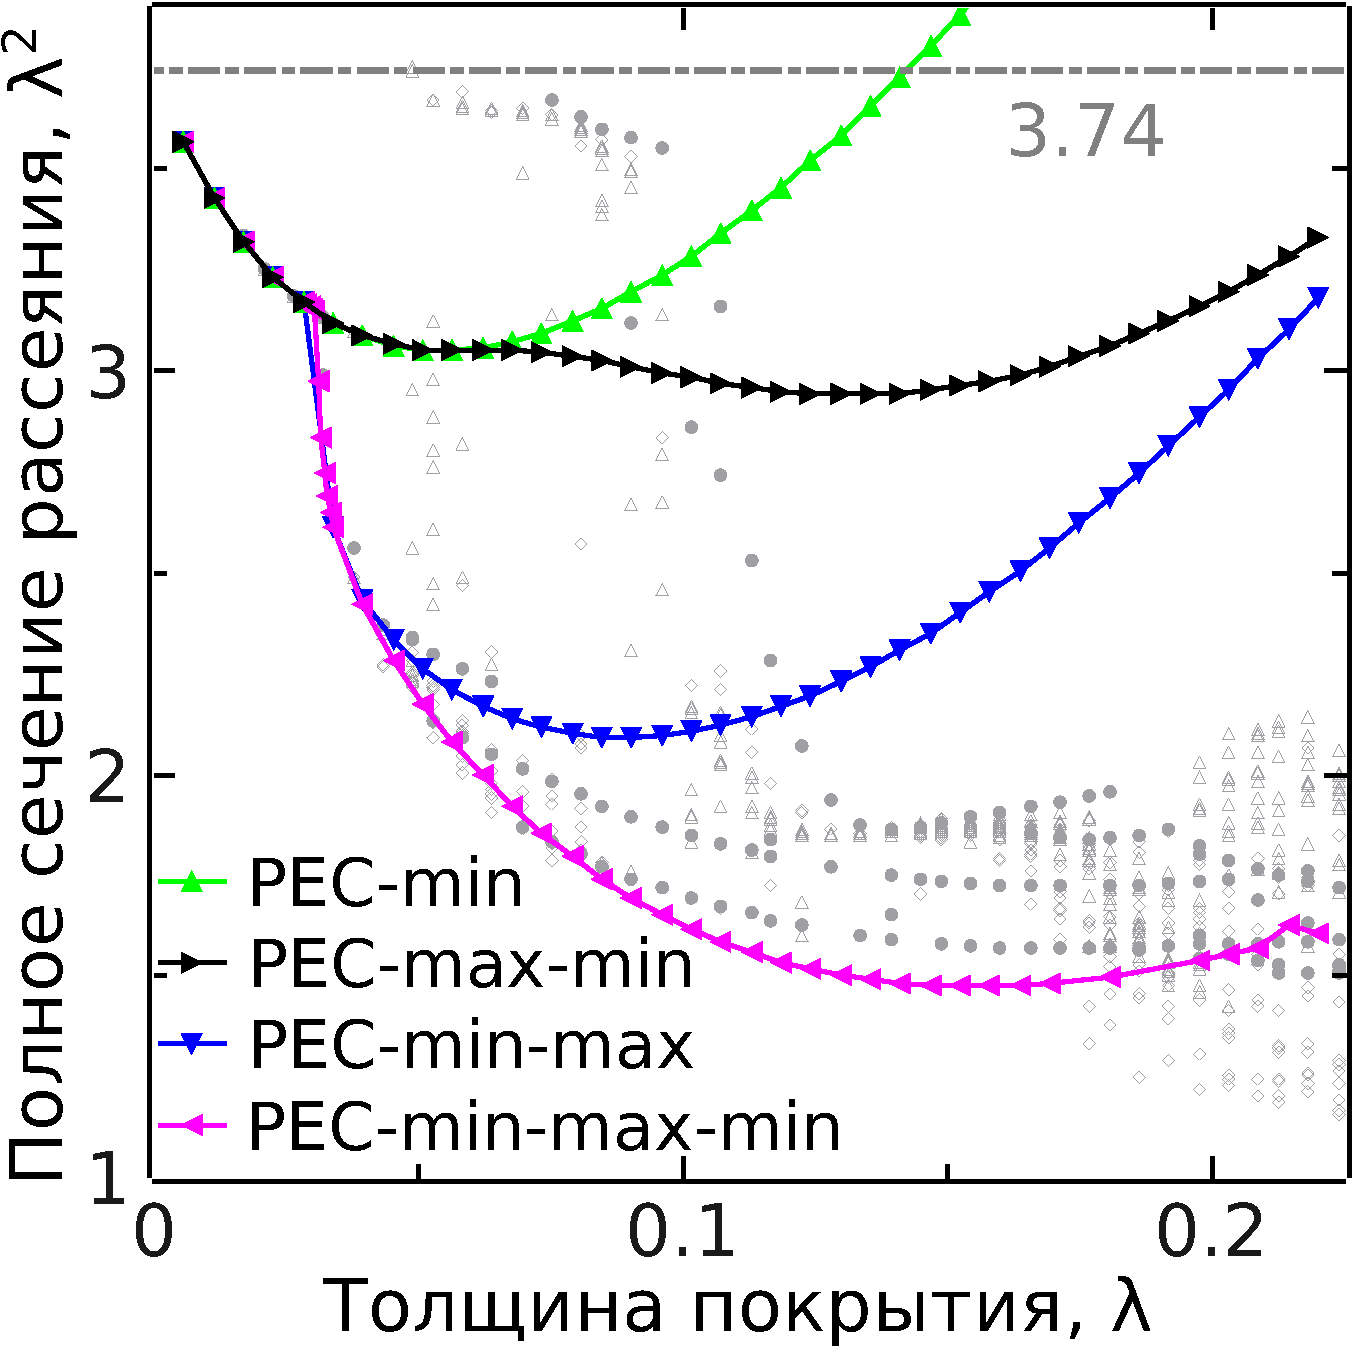
\includegraphics[width=0.95\linewidth]{rcs-overview-index07-DI} \\ а)}
  \end{minipage}
  \hfill
  \begin{minipage}[ht]{0.49\linewidth}
    \centering{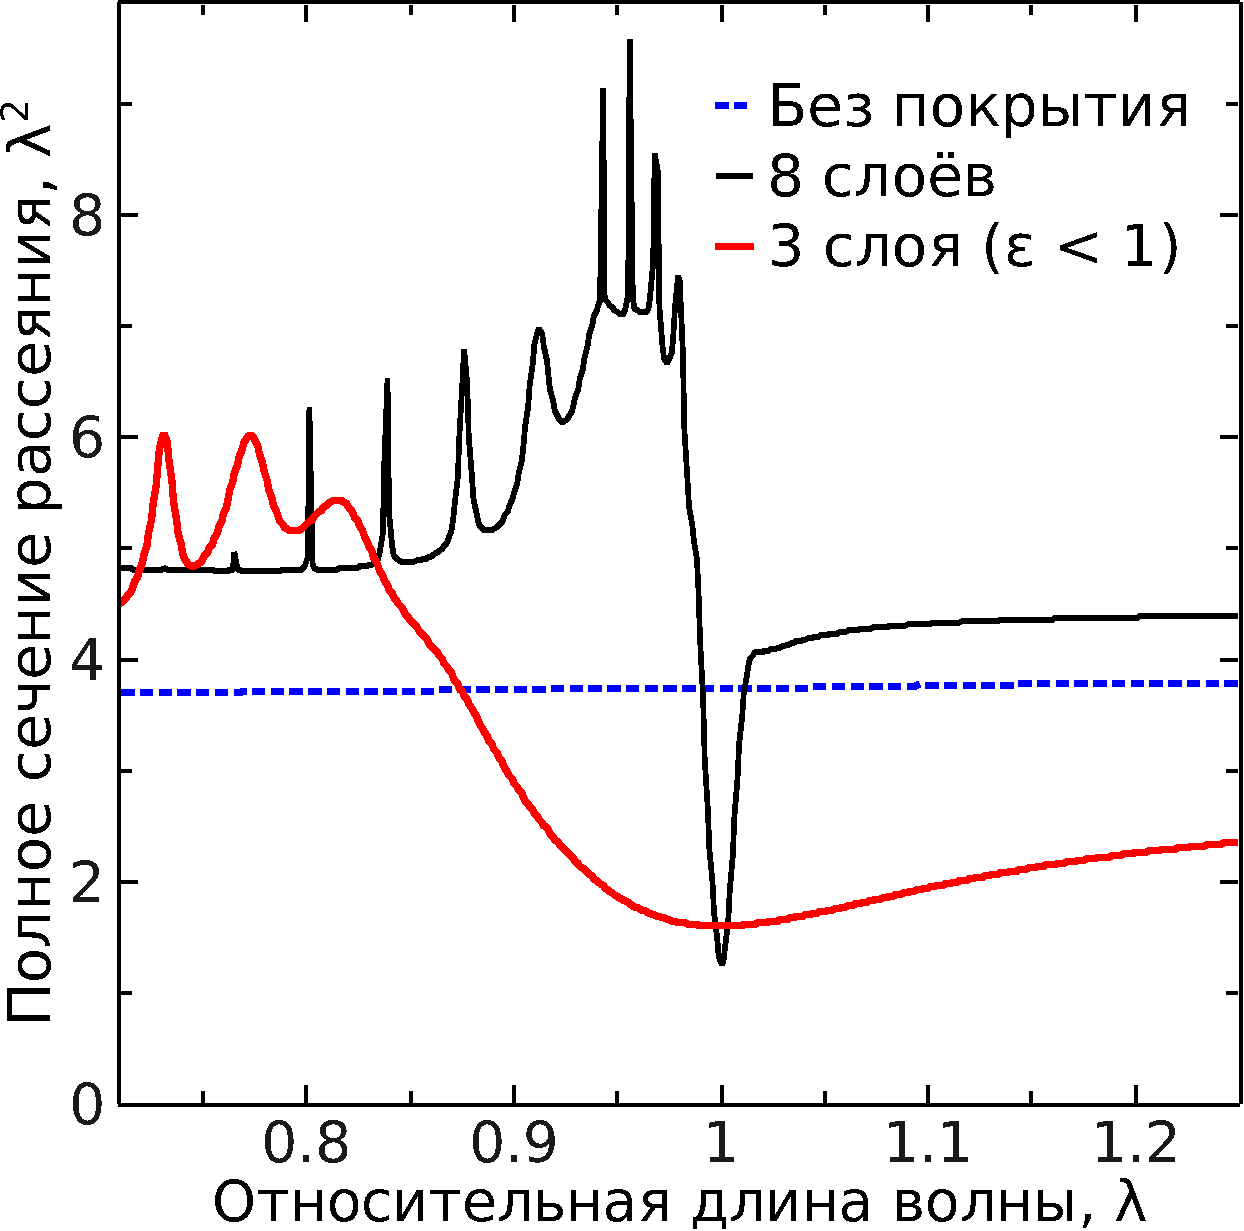
\includegraphics[width=0.95\linewidth]{index07-spectra} \\ б)}
  \end{minipage}
  \caption{а) Результат оптимизации покрытий с чередующимися слоями из
    большого $\varepsilon$ и ${\varepsilon<1}$. б) Спектры частицы
  без покрытия и с маскирующими покрытиями: из 8-ми слоёв диэлектрика и
  из 3-х слоёв с применением ${\varepsilon<1}$.}
  \label{img:min-max-min}  
\end{figure}

Обнаруженная закономерность позволила сформулировать гипотезу,
что для создания маскирующего покрытия достаточно использовать всего
два материала: с большим $\varepsilon$ и ${\varepsilon<1}$, а в
качестве параметров оптимизации можно использовать толщину каждого
слоя. Эта гипотеза была проверена численно, результаты оптимизации
отображены на рисунке~\ref{img:min-max-min}(а). Оказалось, что для
большей части рассматриваемого диапазона общей толщины покрытия 
достаточно всего трёх слоёв, чтобы получить приблизительно то же
уменьшение полного сечения рассеяния, что и в случае применения 4, 8 и
16 слоёв равной толщины, когда при оптимизации
изменялись материальные параметры каждого слоя.

Особый интерес представляет различие в спектрах рассеяния для случаев
наличия и отсутствия материала с ${\varepsilon<1}$ в оптимизированном
покрытии.  При расчёте спектров для рисунка~\ref{img:min-max-min}(б) не
учитывалось наличие в материалах дисперсии и сопутствующих потерь,
поэтому их форма полностью определяется дизайном маскирующего
покрытия. Хорошо виден относительно узкий резонанс, который определяет
маскирующие свойства покрытия на основе диэлектриков. Использование
материала с ${\varepsilon<1}$ позволило в несколько раз расширить
диапазон длин волн, где наблюдается подавление рассеяния. 

\clearpage           % Глава 3
\chapter*{Заключение}						% Заголовок
\addcontentsline{toc}{chapter}{Заключение}	% Добавляем его в оглавление

%% Согласно ГОСТ Р 7.0.11-2011:
%% 5.3.3 В заключении диссертации излагают итоги выполненного исследования, рекомендации, перспективы дальнейшей разработки темы.
%% 9.2.3 В заключении автореферата диссертации излагают итоги данного исследования, рекомендации и перспективы дальнейшей разработки темы.
%% Поэтому имеет смысл сделать эту часть общей и загрузить из одного файла в автореферат и в диссертацию:

Основные результаты работы заключаются в следующем:
%% Согласно ГОСТ Р 7.0.11-2011:
%% 5.3.3 В заключении диссертации излагают итоги выполненного исследования, рекомендации, перспективы дальнейшей разработки темы.
%% 9.2.3 В заключении автореферата диссертации излагают итоги данного исследования, рекомендации и перспективы дальнейшей разработки темы.
\begin{enumerate}
  \item Предложен метод изучения экстремальных оптических свойств
    многослойных сферических наночастиц с помощью теории Ми и
    стохастической оптимизации. Высокая вычислительная
    производительность этого подхода позволила выявить несколько новых
    физических эффектов, связанных с рассеянием и поглощением
    электромагнитной волны на многослойных сферических наночастицах.
  \item В задаче рассеяния плоской волны на многослойной сфере
    получены явные рекуррентные соотношения для коэффициентов Ми в
    расчёте локальных полей, выраженные через логарифмические
    производные функций Риккати-Бесселя.  Эти соотношения были
    добавлены в компьютерную программу, выполняющую вычисления в
    рамках задачи Ми.
  \item Рассеяние от объекта из идеального проводника можно
    существенно уменьшить с помощью многослойного покрытия толщиной
    $0.15\lambda$, используя только изотропные диэлектрические
    материалы: в 2 и в 6 раз для объектов диаметром $1.5\lambda$ и
    $\lambda/1.5$ соответственно. Обнаружен пороговый характер
    уменьшения рассеяния в зависимости от толщины покрытия.
  \item % (TODO берем балошени без слов min-max-min)
    Среди разнообразных оптимизированных дизайнов маскирующих покрытий из
    изотропных материалов с $\varepsilon$ меньше единицы, состоящих из
    множества слоёв равной толщины, выявлена закономерность,
    позволяющая разрабатывать эффективные трёхслойные сферические
    покрытия с разными толщинами слоёв. Дополнительной особенностью
    таких покрытий является значительное увеличение области спектра, в
    которой наблюдается эффект маскировки, при сравнении с покрытиями
    из диэлектриков. 
    %%%%%% Спектр --- засада
  \item В трёхслойных частицах $Si/Ag/Si$ возможно вырождение
    мультипольных резонансов, приводящее к эффекту суперпоглощения,
    когда сечение поглощения оказывается больше, чем у однородной
    частицы того же размера из произвольного изотропного
    материала. Максимальная эффективность поглощения в
    рассматриваемой системе была получена для небольших двухслойных
    частиц с преобладающей ролью электрического дипольного резонанса.
\end{enumerate}

И какая-нибудь заключающая фраза и благодарности.
      % Заключение
\clearpage                                  % В том числе гарантирует, что список литературы в оглавлении будет с правильным номером страницы
%\hypersetup{ urlcolor=black }               % Ссылки делаем чёрными
%\providecommand*{\BibDash}{}                % В стилях ugost2008 отключаем использование тире как разделителя 
\urlstyle{rm}                               % ссылки URL обычным шрифтом
\insertbibliofull                          % Подключаем Bib-базы
\urlstyle{tt}                               % возвращаем установки шрифта ссылок URL
%\hypersetup{ urlcolor={urlcolor} }          % Восстанавливаем цвет ссылок      % Список литературы
\clearpage
\ifthenelse{\NOT \isundefined{\microtypesetup}}{\microtypesetup{protrusion=false}}{} % не рекомендуется применять пакет микротипографики к автоматически генерируемым спискам
\listoffigures  % Список изображений

%%% Список таблиц %%%
% (ГОСТ Р 7.0.11-2011, 5.3.10)
\clearpage
\listoftables   % Список таблиц
\ifthenelse{\NOT \isundefined{\microtypesetup}}{\microtypesetup{protrusion=true}}{}
\newpage           % Списки таблиц и изображений (иллюстративный материал)
% \appendix
%%% Оформление заголовков приложений ближе к ГОСТ:
\setlength{\midchapskip}{20pt}
\renewcommand*{\afterchapternum}{\par\nobreak\vskip \midchapskip}
\renewcommand\thechapter{\Asbuk{chapter}} % Чтобы приложения русскими буквами нумеровались
   % Предварительные настройки для правильного подключения Приложений
% \chapter{Примеры вставки листингов программного кода} \label{AppendixA}

% Для крупных листингов есть два способа. Первый красивый, но в нём могут быть проблемы с поддержкой кириллицы (у вас может встречаться в комментариях и
% печатаемых сообщениях), он представлен на листинге~\ref{list:hwbeauty}.
% %\renewcommand\FBbskip{-20pt} % если хотим притянуть что-то к плавающему окружению из floatrow
% \begin{ListingEnv}[H]% буква H означает Here, ставим здесь,
%     % элементы, которые нежелательно разрывать обычно не ставят
%     % посреди страницы: вместо H используется t (top, сверху страницы),
%     % или b (bottom) или p (page, на отдельной странице)
% %    \captionsetup{format=tablenocaption}% должен стоять до самого caption
% %    \thisfloatsetup{\capposition=top}%
%     \caption{Программа “Hello, world” на \protect\cpp}
%     % далее метка для ссылки:
%     \label{list:hwbeauty}
%     % окружение учитывает пробелы и табляции и приеняет их в сответсвии с настройкми
%     \begin{lstlisting}[language={[ISO]C++}]
% 	#include <iostream>
% 	using namespace std;

% 	int main() //кириллица в комментариях при xelatex и lualatex имеет проблемы с пробелами
% 	{
% 		cout << "Hello, world" << endl; //latin letters in commentaries
% 		system("pause");
% 		return 0;
% 	}
%     \end{lstlisting}
% \end{ListingEnv}%
% Второй не такой красивый, но без ограничений (см.~листинг~\ref{list:hwplain}).
% \begin{ListingEnv}[H]
%     \begin{Verb}
        
%         #include <iostream>
%         using namespace std;
        
%         int main() //кириллица в комментариях
%         {
%             cout << "Привет, мир" << endl;
%         }
%     \end{Verb}
%     \caption{Программа “Hello, world” без подсветки}
%     \label{list:hwplain}
% \end{ListingEnv}

% Можно использовать первый для вставки небольших фрагментов
% внутри текста, а второй для вставки полного
% кода в приложении, если таковое имеется.

% Если нужно вставить совсем короткий пример кода (одна или две строки), то выделение  линейками и нумерация может смотреться чересчур громоздко. В таких случаях можно использовать окружения \texttt{lstlisting} или \texttt{Verb} без \texttt{ListingEnv}. Приведём такой пример с указанием языка программирования, отличного от заданного по умолчанию:
% \begin{lstlisting}[language=Haskell]
% fibs = 0 : 1 : zipWith (+) fibs (tail fibs)
% \end{lstlisting}
% Такое решение~--- со вставкой нумерованных листингов покрупнее
% и вставок без выделения для маленьких фрагментов~--- выбрано,
% например, в книге Эндрю Таненбаума и Тодда Остина по архитектуре
% %компьютера~\autocite{TanAus2013} (см.~рис.~\ref{fig:tan-aus}).

% Наконец, для оформления идентификаторов внутри строк
% (функция \lstinline{main} и тому подобное) используется
% \texttt{lstinline} или, самое простое, моноширинный текст
% (\texttt{\textbackslash texttt}).


% Пример~\ref{list:internal3}, иллюстрирующий подключение переопределённого языка. Может быть полезным, если подсветка кода работает криво. Без дополнительного окружения, с подписью и ссылкой, реализованной встроенным средством.
% \begin{lstlisting}[language={Renhanced},caption={Пример листинга c подписью собственными средствами},label={list:internal3}]
% ## Caching the Inverse of a Matrix

% ## Matrix inversion is usually a costly computation and there may be some
% ## benefit to caching the inverse of a matrix rather than compute it repeatedly
% ## This is a pair of functions that cache the inverse of a matrix.

% ## makeCacheMatrix creates a special "matrix" object that can cache its inverse

% makeCacheMatrix <- function(x = matrix()) {#кириллица в комментариях при xelatex и lualatex имеет проблемы с пробелами
%     i <- NULL
%     set <- function(y) {
%         x <<- y
%         i <<- NULL
%     }
%     get <- function() x
%     setSolved <- function(solve) i <<- solve
%     getSolved <- function() i
%     list(set = set, get = get,
%     setSolved = setSolved,
%     getSolved = getSolved)
    
% }


% ## cacheSolve computes the inverse of the special "matrix" returned by
% ## makeCacheMatrix above. If the inverse has already been calculated (and the
% ## matrix has not changed), then the cachesolve should retrieve the inverse from
% ## the cache.

% cacheSolve <- function(x, ...) {
%     ## Return a matrix that is the inverse of 'x'
%     i <- x$getSolved()
%     if(!is.null(i)) {
%         message("getting cached data")
%         return(i)
%     }
%     data <- x$get()
%     i <- solve(data, ...)
%     x$setSolved(i)
%     i  
% }
% \end{lstlisting} %$ %Комментарий для корректной подсветки синтаксиса
%                  %вне листинга

% Листинг~\ref{list:external1} подгружается из внешнего файла. Приходится загружать без окружения дополнительного. Иначе по страницам не переносится.
%     \lstinputlisting[lastline=78,language={R},caption={Листинг из внешнего файла},label={list:external1}]{listings/run_analysis.R}






% \chapter{Очень длинное название второго приложения, в котором продемонстрирована работа с длинными таблицами} \label{AppendixB}

% \normalsize% возвращаем шрифт к нормальному
% \section{Ещё один подраздел приложения} \label{AppendixB2}

% Нужно больше подразделов приложения!

% Пример длинной таблицы с записью продолжения по ГОСТ 2.105

%     \centering
% 	\small
%     \begin{longtable}[c]{|l|c|l|l|}
% 	\caption{Наименование таблицы средней длины}%
%     \label{tbl:test5}% label всегда желательно идти после caption
%     \\
%     \hline
%      %\multicolumn{4}{|c|}{\textbf{Файл puma\_namelist}}        \\ \hline
%      Параметр & Умолч. & Тип & Описание\\ \hline
%      \endfirsthead%
% %     \multicolumn{4}{|c|}{\small\slshape (продолжение)}        \\ \hline
%  \captionsetup{format=tablenocaption,labelformat=continued}% должен стоять до самого caption
%     \caption[]{}\\
%     \hline
%      Параметр & Умолч. & Тип & Описание\\ \hline
%       \endhead
%       \hline
% %     \multicolumn{4}{|r|}{\small\slshape продолжение следует}  \\
% %\hline
%      \endfoot
%          \hline
%      \endlastfoot
%      \multicolumn{4}{|l|}{\&INP}        \\ \hline 
%      kick & 1 & int & 0: инициализация без шума ($p_s = const$) \\
%           &   &     & 1: генерация белого шума                  \\
%           &   &     & 2: генерация белого шума симметрично относительно \\
%       & & & экватора    \\
%      mars & 0 & int & 1: инициализация модели для планеты Марс     \\
%      kick & 1 & int & 0: инициализация без шума ($p_s = const$) \\
%           &   &     & 1: генерация белого шума                  \\
%           &   &     & 2: генерация белого шума симметрично относительно \\
%       & & & экватора    \\
%      mars & 0 & int & 1: инициализация модели для планеты Марс     \\
%     kick & 1 & int & 0: инициализация без шума ($p_s = const$) \\
%           &   &     & 1: генерация белого шума                  \\
%           &   &     & 2: генерация белого шума симметрично относительно \\
%       & & & экватора    \\
%      mars & 0 & int & 1: инициализация модели для планеты Марс     \\
%     kick & 1 & int & 0: инициализация без шума ($p_s = const$) \\
%           &   &     & 1: генерация белого шума                  \\
%           &   &     & 2: генерация белого шума симметрично относительно \\
%       & & & экватора    \\
%      mars & 0 & int & 1: инициализация модели для планеты Марс     \\
%     kick & 1 & int & 0: инициализация без шума ($p_s = const$) \\
%           &   &     & 1: генерация белого шума                  \\
%           &   &     & 2: генерация белого шума симметрично относительно \\
%       & & & экватора    \\
%      mars & 0 & int & 1: инициализация модели для планеты Марс     \\
%     kick & 1 & int & 0: инициализация без шума ($p_s = const$) \\
%           &   &     & 1: генерация белого шума                  \\
%           &   &     & 2: генерация белого шума симметрично относительно \\
%       & & & экватора    \\
%      mars & 0 & int & 1: инициализация модели для планеты Марс     \\
%     kick & 1 & int & 0: инициализация без шума ($p_s = const$) \\
%           &   &     & 1: генерация белого шума                  \\
%           &   &     & 2: генерация белого шума симметрично относительно \\
%       & & & экватора    \\
%      mars & 0 & int & 1: инициализация модели для планеты Марс     \\
%     kick & 1 & int & 0: инициализация без шума ($p_s = const$) \\
%           &   &     & 1: генерация белого шума                  \\
%           &   &     & 2: генерация белого шума симметрично относительно \\
%       & & & экватора    \\
%      mars & 0 & int & 1: инициализация модели для планеты Марс     \\
%     kick & 1 & int & 0: инициализация без шума ($p_s = const$) \\
%           &   &     & 1: генерация белого шума                  \\
%           &   &     & 2: генерация белого шума симметрично относительно \\
%       & & & экватора    \\
%      mars & 0 & int & 1: инициализация модели для планеты Марс     \\
%     kick & 1 & int & 0: инициализация без шума ($p_s = const$) \\
%           &   &     & 1: генерация белого шума                  \\
%           &   &     & 2: генерация белого шума симметрично относительно \\
%       & & & экватора    \\
%      mars & 0 & int & 1: инициализация модели для планеты Марс     \\
%     kick & 1 & int & 0: инициализация без шума ($p_s = const$) \\
%           &   &     & 1: генерация белого шума                  \\
%           &   &     & 2: генерация белого шума симметрично относительно \\
%       & & & экватора    \\
%      mars & 0 & int & 1: инициализация модели для планеты Марс     \\
%     kick & 1 & int & 0: инициализация без шума ($p_s = const$) \\
%           &   &     & 1: генерация белого шума                  \\
%           &   &     & 2: генерация белого шума симметрично относительно \\
%       & & & экватора    \\
%      mars & 0 & int & 1: инициализация модели для планеты Марс     \\
%     kick & 1 & int & 0: инициализация без шума ($p_s = const$) \\
%           &   &     & 1: генерация белого шума                  \\
%           &   &     & 2: генерация белого шума симметрично относительно \\
%       & & & экватора    \\
%      mars & 0 & int & 1: инициализация модели для планеты Марс     \\
%     kick & 1 & int & 0: инициализация без шума ($p_s = const$) \\
%           &   &     & 1: генерация белого шума                  \\
%           &   &     & 2: генерация белого шума симметрично относительно \\
%       & & & экватора    \\
%      mars & 0 & int & 1: инициализация модели для планеты Марс     \\
%     kick & 1 & int & 0: инициализация без шума ($p_s = const$) \\
%           &   &     & 1: генерация белого шума                  \\
%           &   &     & 2: генерация белого шума симметрично относительно \\
%       & & & экватора    \\
%      mars & 0 & int & 1: инициализация модели для планеты Марс     \\
%      \hline
%       %& & & $\:$ \\ 
%      \multicolumn{4}{|l|}{\&SURFPAR}        \\ \hline
%     kick & 1 & int & 0: инициализация без шума ($p_s = const$) \\
%           &   &     & 1: генерация белого шума                  \\
%           &   &     & 2: генерация белого шума симметрично относительно \\
%       & & & экватора    \\
%      mars & 0 & int & 1: инициализация модели для планеты Марс     \\
%     kick & 1 & int & 0: инициализация без шума ($p_s = const$) \\
%           &   &     & 1: генерация белого шума                  \\
%           &   &     & 2: генерация белого шума симметрично относительно \\
%       & & & экватора    \\
%      mars & 0 & int & 1: инициализация модели для планеты Марс     \\
%     kick & 1 & int & 0: инициализация без шума ($p_s = const$) \\
%           &   &     & 1: генерация белого шума                  \\
%           &   &     & 2: генерация белого шума симметрично относительно \\
%       & & & экватора    \\
%      mars & 0 & int & 1: инициализация модели для планеты Марс     \\
%     kick & 1 & int & 0: инициализация без шума ($p_s = const$) \\
%           &   &     & 1: генерация белого шума                  \\
%           &   &     & 2: генерация белого шума симметрично относительно \\
%       & & & экватора    \\
%      mars & 0 & int & 1: инициализация модели для планеты Марс     \\
%     kick & 1 & int & 0: инициализация без шума ($p_s = const$) \\
%           &   &     & 1: генерация белого шума                  \\
%           &   &     & 2: генерация белого шума симметрично относительно \\
%       & & & экватора    \\
%      mars & 0 & int & 1: инициализация модели для планеты Марс     \\
%     kick & 1 & int & 0: инициализация без шума ($p_s = const$) \\
%           &   &     & 1: генерация белого шума                  \\
%           &   &     & 2: генерация белого шума симметрично относительно \\
%       & & & экватора    \\
%      mars & 0 & int & 1: инициализация модели для планеты Марс     \\
%     kick & 1 & int & 0: инициализация без шума ($p_s = const$) \\
%           &   &     & 1: генерация белого шума                  \\
%           &   &     & 2: генерация белого шума симметрично относительно \\
%       & & & экватора    \\
%      mars & 0 & int & 1: инициализация модели для планеты Марс     \\
%     kick & 1 & int & 0: инициализация без шума ($p_s = const$) \\
%           &   &     & 1: генерация белого шума                  \\
%           &   &     & 2: генерация белого шума симметрично относительно \\
%       & & & экватора    \\
%      mars & 0 & int & 1: инициализация модели для планеты Марс     \\
%     kick & 1 & int & 0: инициализация без шума ($p_s = const$) \\
%           &   &     & 1: генерация белого шума                  \\
%           &   &     & 2: генерация белого шума симметрично относительно \\
%       & & & экватора    \\
%      mars & 0 & int & 1: инициализация модели для планеты Марс     \\ 
% %     \hline 
%     \end{longtable}
% \normalsize% возвращаем шрифт к нормальному
% \section{Очередной подраздел приложения} \label{AppendixB3}

% Нужно больше подразделов приложения!

% \section{И ещё один подраздел приложения} \label{AppendixB4}

% Нужно больше подразделов приложения!

        % Приложения

\end{document}
